%---------------------------------------------------------------------------%
%-                                                                         -%
%-                           LaTeX Template                                -%
%-                                                                         -%
%---------------------------------------------------------------------------%
%- Copyright (C) Huangrui Mo <huangrui.mo@gmail.com> 
%- This is free software: you can redistribute it and/or modify it
%- under the terms of the GNU General Public License as published by
%- the Free Software Foundation, either version 3 of the License, or
%- (at your option) any later version.
%---------------------------------------------------------------------------%
%->> Document class declaration
%---------------------------------------------------------------------------%
\documentclass[twoside]{Style/ucasthesis}%
%- Multiple optional arguments:
%- [<oneside|twoside|print>]% oneside eprint, twoside eprint, or paper print
%- [fontset=<adobe|...>]% specify font set to replace automatic detection
%- [plain]% thesis writing of international students
%- [draftversion]% show draft version information
%- [standard options for ctex book class: draft|paper size|font size|...]%
%---------------------------------------------------------------------------%
%->> Document settings
%---------------------------------------------------------------------------%
\usepackage[authoryear,list]{Style/artratex}% document settings
%- usage: \usepackage[option1,option2,...,optionN]{artratex}
%- Multiple optional arguments:
%- [bibtex|biber]% set bibliography processor and package
%- [<numbers|super|authoryear|alpha>]% set citation and reference style
%- <numbers>: textual: Jones [1]; parenthetical: [1]
%- <super>: textual: Jones superscript [1]; parenthetical: superscript [1]
%- <authoryear>: textual: Jones (1995); parenthetical: (Jones, 1995)
%- <alpha>: textual: not available; parenthetical: [Jon95]
%- [geometry]% reconfigure page layout via geometry package
%- [lscape]% provide landscape layout environment
%- [xhf]% disable header and footer via fancyhdr package
%- [color]% provide color support via xcolor package
%- [background]% enable page background
%- [tikz]% provide complex diagrams via tikz package
%- [table]% provide complex tables via ctable package
%- [list]% provide enhanced list environments for algorithm and coding
%- [math]% enable some extra math packages
%- [xlink]% disable link colors
\usepackage{Style/artracom}% user defined commands
%---------------------------------------------------------------------------%
%->> Document inclusion
%---------------------------------------------------------------------------%
%\includeonly{Tex/Chap_1,...,Tex/Chap_N}% selected files compilation
%---------------------------------------------------------------------------%
%->> Document content
%---------------------------------------------------------------------------%
%-
%-> Titlepage information
%-
%---------------------------------------------------------------------------%
%->> Titlepage information
%---------------------------------------------------------------------------%
%-
%-> 中文封面信息
%-
\confidential{}% 密级:只有涉密论文才填写
\schoollogo[scale=0.095]{ucas_logo}% 校徽
\title{数据流计算模型}% 论文中文题目
\author{莫晃锐}% 论文作者
\advisor{刘青泉~研究员~中国科学院力学研究所}% 指导教师:姓名 专业技术职务 工作单位
\advisors{}% 指导老师附加信息 或 第二指导老师信息
\degree{硕士}% 学位:学士、硕士、博士
\degreetype{理学}% 学位类别:理学、工学、工程、医学等
\major{流体力学}% 二级学科专业名称
\institute{中国科学院力学研究所}% 院系名称
\date{2014~年~6~月}% 毕业日期:夏季为6月、冬季为12月
%-
%-> 英文封面信息
%-
\TITLE{\LaTeX{} Thesis Template\\ of \\ The University of Chinese Academy of Sciences {$~^{\pi}\pi^{\pi}$}}% 论文英文题目
\AUTHOR{Mo Huangrui}% 论文作者
\ADVISOR{Supervisor: Professor Liu Qingquan}% 指导教师
\DEGREE{Master}% 学位:Bachelor, Master, Doctor, Postdoctor。封面据英文学位名称自动切换,需确保拼写准确
\DEGREETYPE{Natural Science}% 学位类别:Philosophy, Natural Science, Engineering, Economics, Agriculture 等
\MAJOR{Fluid Mechanics}% 二级学科专业名称
\INSTITUTE{Institute of Mechanics, Chinese Academy of Sciences}% 院系名称
\DATE{June, 2014}% 毕业日期:夏季为June、冬季为December
%---------------------------------------------------------------------------%
%
\begin{document}
%-
%-> Frontmatter: title page, abstract, content list, symbol list, preface
%-

\frontmatter% initialize the environment

%---------------------------------------------------------------------------%
%->> Frontmatter
%---------------------------------------------------------------------------%
%-
%-> 生成封面
%-
%%\maketitle% 生成中文封面

%%-----------------------------------------%%
%% 中文封面
\pagestyle{empty}  %% 不要页眉页脚(临时添加)

\vspace*{3cm}
\center{\Huge{数据流计算模型}} \\ 
\center{\huge{(卷B)}}

\vspace*{5cm}
\center{\Large{高光荣,杰克·丹尼斯\ 等著}}

\vspace*{8cm}
\center{\large{<出版社>}}
%%-----------------------------------------%%

%%\MAKETITLE% 生成英文封面
%-
%-> 作者声明
%-
%%\makedeclaration% 生成声明页

%-
%-> 中文摘要
%-
%%\intobmk\chapter*{摘\quad 要}% 显示在书签但不显示在目录
%%\setcounter{page}{1}% 开始页码
%%\pagenumbering{Roman}% 页码符号

%%本文是中国科学院大学学位论文模板ucasthesis的使用说明文档。主要内容为介绍\LaTeX{}文档类ucasthesis的用法,以及如何使用\LaTeX{}快速高效地撰写学位论文。

%%\keywords{中国科学院大学,学位论文,\LaTeX{}模板}% 中文关键词

%-
%-> 英文摘要
%-
%%\intobmk\chapter*{Abstract}% 显示在书签但不显示在目录

%%This paper is a help documentation for the \LaTeX{} class ucasthesis, which is  a thesis template for the University of Chinese Academy of Sciences. The main content is about how to use the ucasthesis, as well as how to write thesis efficiently by using \LaTeX{}.

%%\KEYWORDS{University of Chinese Academy of Sciences (UCAS), Thesis, \LaTeX{} Template}% 英文关键词
%---------------------------------------------------------------------------%

%%-----------------------------------------%%
%% 贡献者
\intobmk\chapter*{本书贡献者列表(卷B)}% 显示在书签但不显示在目录
\setcounter{page}{1}% 开始页码
\pagenumbering{Roman}% 页码符号

\begin{flushleft}  %% 左对其(临时添加)
\setlength{\parindent}{2em} %% 首行缩进(临时添加)

贡献者列表......

\end{flushleft}
%%-----------------------------------------%%

%%-----------------------------------------%%
%% 序言
\chapter{前\quad 言}% 显示在书签

<作者:待定>
\begin{flushleft}  %% 左对其(临时添加)
\setlength{\parindent}{2em} %% 首行缩进(临时添加)

前言内容......

\end{flushleft}
%%-----------------------------------------%%

% title page, abstract
{% content list region
\linespread{1.2}% local line space
\intobmk*{\cleardoublepage}{\contentsname}% add link to bookmark
\tableofcontents% content catalog

%%\intobmk*{\cleardoublepage}{\listfigurename}% add link to bookmark
%%\listoffigures% figure catalog
%%\intobmk*{\cleardoublepage}{\listtablename}% add link to bookmark
%%\listoftables% table catalog
}
%%\intobmk\chapter*{符号列表}% 显示在书签但不显示在目录

\section*{字符}
\nomenclatureitem[\textbf{Unit}]{\textbf{Symbol}}{\textbf{Description}}
\nomenclatureitem[$\Unit{m^{2} \cdot s^{-2} \cdot K^{-1}}$]{$R$}{the gas constant}
\nomenclatureitem[$\Unit{m^{2} \cdot s^{-2} \cdot K^{-1}}$]{$C_v$}{specific heat capacity at constant volume}
\nomenclatureitem[$\Unit{m^{2} \cdot s^{-2} \cdot K^{-1}}$]{$C_p$}{specific heat capacity at constant pressure}
\nomenclatureitem[$\Unit{m^{2} \cdot s^{-2}}$]{$E$}{specific total energy}
\nomenclatureitem[$\Unit{m^{2} \cdot s^{-2}}$]{$e$}{specific internal energy}
\nomenclatureitem[$\Unit{m^{2} \cdot s^{-2}}$]{$h_T$}{specific total enthalpy}
\nomenclatureitem[$\Unit{m^{2} \cdot s^{-2}}$]{$h$}{specific enthalpy}
\nomenclatureitem[$\Unit{kg \cdot m \cdot s^{-3} \cdot K^{-1}}$]{$k$}{thermal conductivity}
\nomenclatureitem[$\Unit{kg \cdot m^{-1} \cdot s^{-2}}$]{$S_{ij}$}{deviatoric stress tensor}
\nomenclatureitem[$\Unit{kg \cdot m^{-1} \cdot s^{-2}}$]{$\tau_{ij}$}{viscous stress tensor}
\nomenclatureitem[$\Unit{1}$]{$\delta_{ij}$}{Kronecker tensor}
\nomenclatureitem[$\Unit{1}$]{$I_{ij}$}{identity tensor}

\section*{算子}
\nomenclatureitem{\textbf{Symbol}}{\textbf{Description}}
\nomenclatureitem{$\Delta$}{difference}
\nomenclatureitem{$\nabla$}{gradient operator}
\nomenclatureitem{$\delta^{\pm}$}{upwind-biased interpolation scheme}

\section*{缩写}
\nomenclatureitem{CFD}{Computational Fluid Dynamics}
\nomenclatureitem{CFL}{Courant-Friedrichs-Lewy}
\nomenclatureitem{EOS}{Equation of State}
\nomenclatureitem{JWL}{Jones-Wilkins-Lee}
\nomenclatureitem{WENO}{Weighted Essentially Non-oscillatory}
\nomenclatureitem{ZND}{Zel'dovich-von Neumann-Doering}

% symbol list, preface content

%%-----------------------------------------%%
%% 序言
\chapter*{序\quad 言} %% 显示在目录
\addcontentsline{toc}{chapter}{序\quad 言} %% 向目录中添加条目,以章的名义(临时添加)

<作者:G.R. Gao and J.B. Dennis>

\begin{flushleft}  %% 左对其(临时添加)
\setlength{\parindent}{2em} %% 首行缩进(临时添加)

序言内容......

\end{flushleft}
%%-----------------------------------------%%




%-
%-> Mainmatter
%-
\mainmatter% initialize the environment
%---------------------------------------------------------------------------%
%->> Main content
%---------------------------------------------------------------------------%

\chapter{数据流计算模型——入门}\label{chap:primer} %%第一章
\chapter{程序执行模型和编程模型}\label{chap:model} %%第二章
\chapter{结构与芯片设计}\label{chap:arch}
 %%第三章
\chapter{算法与实现}\label{chap:algo}

\begin{flushleft}  %% 左对其(临时添加)
\setlength{\parindent}{2em} %% 首行缩进(临时添加)

\qquad  

过去十年来高性能计算经历了从十万亿次到百万亿次再到千万亿次的突破,高性能算法设计与优化面临着利用并行性(并行墙)和开发局部性(内存墙)的难题,增加并行度和更深的内存层次可持续提升高性能计算机系统性能,同时对高性能算法设计带来了新挑战,尤其是多核、众核引入的多层次大规模并行(并行墙)并导致内存到计算部件供数不足的问题(内存墙)愈加恶化,因此,如何缓解扩展并行而恶化的访存瓶颈成为高性能计算算法与实现的核心问题,需要通过并行算法模型和实现优化上不断创新。
本章旨在论述数据流思想在解决上述高性能计算关键问题的研究,基于数据流模型,提出适应众核体系结构算法设计和优化的“渗透执行”的算法设计模型,并通过科学计算、组合优化和大数据分析应用的核心算法的实践,展示数据流技术在高性能计算算法设计和优化方面的优势。

\section{导言和背景}
\subsection{导言}
本章介绍基于数据流思想的高性能算法设计和优化技术,其基本动机是众核体系结构发展驱动新的高性能算法模型的提出,渗透模型是其中代表之一。下面几节描述渗透模型及其在典型高性能计算算法中的应用。

关于渗透算法模型的介绍,\ref{sec:percolation}节的逻辑结构是先解释什么是渗透,然后描述如何渗透,包括其基本原理~\ref{sec:percolation_what}、关键技术~\ref{sec:percolation_how}和实现方法~\ref{sec:percolation_method}。

接下来三节展示渗透模型在三个典型算法中的应用,依次是组合优化问题动态规划算法~\ref{sec:PM_dp}、大数据分析图计算~\ref{sec:PM_graph}和科学计算问题稠密矩阵乘~\ref{sec:PM_mm},分别代表了强数据依赖关系、极低数据局部性和规则计算三类问题。从一定程度上验证了基于数据流的渗透模型是一种通用型的高性能算法设计和优化方法。

\subsection{背景}

在高性能计算机系统性能到达P级以后,尤其是以众核为主流的处理器结构的出现,并行性大幅增加,数据通路能力提升缓慢,导致了严重的数据访问(访存、通信)瓶颈,P级应用呈现出数据密集、算法计算访存比低且模式多样的新特点,一味提高硬件系统的峰值性能对实际应用的性能提升帮助不大,算法优化研究成为挖掘高性能计算机实际计算能力的关键,特别是需要适应不同计算访存比的算法优化方法,以提高80\%以上实际应用在“通用型”高性能计算机上的性能。

从高性能算法设计和性能优化的历史角度看,经历了单核、多核和众核三个阶段。在单核处理器结构,算法设计核优化以挖掘程序中的局部性(时间局部性和空间局部性)为核心,重点研究数据布局和存取策略以适应基于cache内存层次的体系结构。到了多核和多处理器时代,并行性的有效挖掘和利用成为关键,提高算法的扩展性是优化的主要目标。众核处理器由于提供了大量的片内并行,局部性和并行性必须是同时考虑的双重目标。纵观已有的执行模型,数据流具有统一局部性和并行性的天然优势。

\begin{figure}[!htbp]
	\centering
	%trim option's parameter order: left bottom right top
	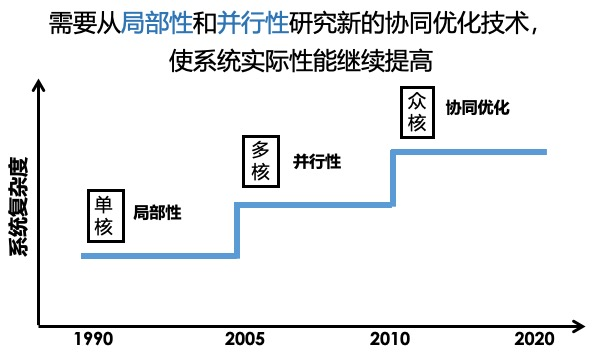
\includegraphics[clip, scale=0.4]{Img/Chap_Algorithm/background}
	\bicaption{性能优化决定了实际峰值。}{Performance optimizations.}
	\label{fig:background}
\end{figure}

\section{基于数据流的高性能算法模型}\label{sec:percolation}

为了缓解日益加剧的“存储墙”(Memory Wall)对高性能算法在多核和众核体系结构上执行性能(计算效率和并行扩展性)的影响,谭光明等~\citep{TanThesis,TanTPDS09}在2008年提出了基于数据流的渗透算法设计模型,以适应高性能计算机系统的计算引擎以众核为主流的趋势。本质上讲,基于数据流的渗透模型(Percolation Model)利用众核体系结构存在的并行为计算操作提供数据访问的局部性,是一种高度融合并行性和局部性的延迟容忍的性能优化技术。本小节从基本原理、关键技术和算法设计方法三个方面介绍渗透模型。

\subsection{渗透模型的基本原理}\label{sec:percolation_what}
从算法设计和优化的角度看,两个主要因素是并行性和局部性。传统的并行算法设计模型中,并行性和局部性是割裂开独立考虑,并行任务的划分和映射仅仅最多考虑到静态数据的亲和性。在数据流执行模型中,并行性和局部性通过以数据为中心而天然统一存在与程序的执行过程中,数据流中actor的firing隐含了所依赖操作并行性和数据局部性的统一,以数据驱动计算的机制执行程序流。基于并行性和局部性统一的数据流思想,面向众核体系结构的渗透模型利用众核天然的并行,实现把数据“推”送到被需要的地方,达到数据驱动计算的效果。

在基于非数据流的执行模型中,每个处理器核在其计算操作执行需要相关数据操作的时刻才发起读取数据的请求,自己从内存中“拉”数据。基于数据流的执行模型,计算操作所依赖的数据通过某种机制在启动计算之前已经被“推”送过来。在集成了大规模片上处理器核的众核架构中,这种“推”送机制可由一些空闲的核完成,因此,在整个程序运行过程中,数据在负责计算操作的处理器核无参与的情况下在不同存储层级中移动,称之为“渗透”(Percolation)。这样在理想情况下,程序的运行过程开销只有有效的计算操作时间。

\begin{figure}[!htbp]
	\centering
	%trim option's parameter order: left bottom right top
	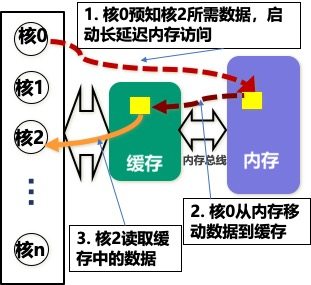
\includegraphics[clip, scale=0.6]{Img/Chap_Algorithm/percolation_what}
	\bicaption{渗透模型的基本原理}{The principle of percolation model.}
	\label{fig:percolation_what}
\end{figure}

如图\ref{fig:percolation_what}所示一个抽象的众核体系结构,众核处理器有$n$个核心,两级内存结构:缓存和内存。“内存墙”瓶颈指的就是通过内存总线访问内存里面的数据,随着处理器中计算核的处理能力增强,性能瓶颈愈加突出。在基于数据流的渗透模型中,在某一个运行时刻,核0主动把核2计算操作所依赖的数据提前从内存移动到缓存中,在核2需要的时候推送给它,这样核2直接从缓存中读取数据,由于在体系结构实现中,缓存通路高带宽和低延迟,从而缓解了“内存墙”的性能瓶颈。

\subsection{渗透模型的关键技术}\label{sec:percolation_how}

渗透模型是为众核体系结构性能优化构建的,多线程是众核体系结构上主流并行机制。在常规的多线程执行中,一旦一个线程需要的数据和控制依赖关系在逻辑上得到满足,该线程就开始启动计算操作。这种弱执行模型对具有高度局部性的规则计算模式能够获得高的性能,然而非规则计算不存在明显的局部性甚至无局部性,弱执行模型不能利用局部性优化提高性能。为了获得非规则计算中的局部性,渗透模型要求线程的执行必须同时满足两个条件:1)数据和控制依赖关系;2)局部性依赖关系(locality dependence)。后者强制线程执行前需要的数据必须位于其局部存储空间中,即渗透模型的关键:即时局部性(just-in-time locality)。

\begin{figure}[!htbp]
	\centering
	%trim option's parameter order: left bottom right top
	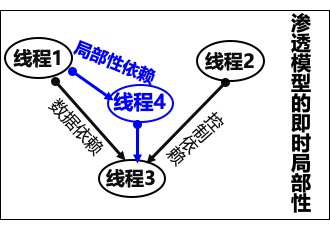
\includegraphics[clip, scale=0.6]{Img/Chap_Algorithm/percolation_how}
	\bicaption{渗透模型的关键技术:即时局部性}{Just-in-time locality.}
	\label{fig:percolation_how}
\end{figure}

在多线程编程模型中,一个线程的工作为一个任务,这样,程序表示成有向无环任务图,图中的顶点表示任务,边代表了两个任务间的依赖关系,如图\ref{fig:percolation_how}。一个顶点$s$(任务/线程)被激活的条件是其前驱操作完成,而且该任务的数据和控制依赖关系得到满足。一个任务仅满足控制和数据依赖关系,称之处于逻辑活跃。在渗透模型中,如果所依赖的数据没有位于待执行任务的局部存储空间,逻辑上活跃的任务不能被调度执行。只有当它的局部性依赖关系得到满足,该逻辑上活跃的任务启动计算。基于众核体系结构的渗透模型中,这种局部性依赖关系由空闲核运行时创建。

为了创建即时局部性,渗透模型要求对算法中的计算和访存操作分离。通过解耦计算和访存,并行算法可以:1)通过访存任务和计算任务之间的多级流水隐藏存储访问的开销;2)组织和分配不同的访存任务来适应存储层次结构中的不同访问延迟,如非连续地址到连续存储区域的变换。在多线程环境中,由某个独立的线程单元称为渗透线程负责存储层次之间的数据移动。尽管渗透在一定程度上与预期机制由共同之处,但又不同于常规的预取,主要体现在下面两个特征:

\begin{itemize}	
	\item {\bf 按需取数}:只有当某个线程需要访问数据时,该数据才出现在片内存储中。如果数据已经在片内存储中,
	该数据马上就会被使用;一段数据的地址即使和刚刚被访问的高延迟存储中的数据的地址连续,如果不需要马上被使用,也不会出现在低延迟存储中。

	\item {\bf 数据变换}:渗透要求在存储层次间聚合/分散数据和对数据组织进行变换,高延迟存储中的离散的存储访问可以在渗透过程中聚合成连续的低延迟存储访问,从而获得局部存储访问的局部性。
\end{itemize}

\subsection{渗透模型的实现方法}\label{sec:percolation_method}

事实上,体系结构支持用户级的计算和访存操作分离已经成为高性能计算机系统的趋势。基于消息传递的并行计算机系统支持零拷贝的RDMA机制(事实上目前
所有的高性能网络设备如Infiniband等都有该特征,并且有相应软件环境),消息传递操作看成访问远程机器的内存。多核结构中通过多线程(如IBM Cyclops64、GPU)或者DMA(如IBM Cell、申威众核)的方式支持异步的存储操作。无论是分布式存储还是共享存储结构,在本文提出抽象机器模型中,
有如下假设:
\begin{itemize}
	\item {\bf 二级存储模型:}所有的处理单元能够直接访问任何的存储空间。相对于每个处理单元,存储空间根据访问延迟的差异划分成延迟相对较低的in-core memory (ICM)和较高的out-of-core memory(OCM),而ICM又可以进一步在多个处理器之间划分成若干in-core local memory(ICLM)。
	\item {\bf 强执行模型:}只有当计算所需要的数据已经在ICM/ICLM时,计算才开始。而且只有当计算的线城需要某数据时,该数据才出现在ICM/ICLM中。
	\item {\bf 细粒度并行:}计算和访问OCM操作能够同时进行
\end{itemize}

通常而言,显式存储层次结构的片内存储比片外存储尺寸小很多,但提供更高的带宽和更低的延迟。目前多核体系结构提供的存储访问延迟容
忍技术主要是多线程和DMA异步传输。如果在两个存储访问之间有足够的计算,则存储访问延迟的问题不会太突出。本章第\ref{sec:PM_graph}介绍的图遍历算法只有少量的计算,
当所有的线程同时访问片外存储时,其延迟和带宽成为性能瓶颈。

在分布式存储体系结构中,节点内部的内存映射为ICM,远程节点的存储映射为OCM;共享存储多核体系结构如IBM
Cyclops64系统中,一个芯片上的SPM和片上SRAM映射为ICM,
SPM可以划分为ICLM,片外DRAM映射为OCM。在基于DMA异步传输的体系结构中,延迟隐藏策略自然地通过DMA实现;多线程体系结构中,需要对线程进行划分,
即分离出一部分线程作为渗透或者{\it helper}线程,这些{\it
	helper}线程负责OCM的访问。在该渗透模型中,通信被抽象为访存操作。

渗透模型强调利用多级并行实现强的执行模型:粗粒度并行用于满足数据和控制依赖关系,细粒度并行获得局部性条件。图~\ref{fig:BasePerc}演示了基本的渗透过程。
{\tiny
	\begin{figure*}[!htbp]
		\begin{center}
			\begin{tabular}{|l|}
				\hline
				\begin{minipage}[t]{4in}
					%{\small
					\begin{tabbing}
						\hspace{.3in} \= {\scshape Percolation Pipelining}\\
						\> XX. \= \kill
						\>  1. \> \b while \= the set of not enabled memory tasks is not empty;\\
						\>       \>\> //stage 1 \\
						\>  2. \> \> A memory tasks $fm(\;)$ becomes enabled;\\
						\>  3. \> \> Data is transformed in off-chip memory;\\
						\>  4. \> \> The transformed data percolates inward to on-chip memory;\\
						\>       \>\> //stage 2 \\
						\>  5. \> \> The code of computation task $fc(\;)$ meeting locality requirement \\
						\>       \>\> percolates inward to on-chip memory;\\
						\>  6. \> \> $fc(\;)$ is enabled;\\
						\>  7. \> \> $fc(\;)$ is retired from on-chip memory;\\
						\>       \>\> //stage 3 \\
						\>  8. \> \> Results are arranged in larger blocks (and transformed)\\
						\>       \> \>  in on-chip memory;\\
						\>  9. \> \> Results are percolated outward to off-chip memory;\\
						\> 10. \> \> Transformations are performed in the outward percolated\\
						\>       \> \>         data in off-chip memory\\
					\end{tabbing}
					%}
				\end{minipage} \\ \hline
			\end{tabular}
			\bicaption{渗透模型流水算法的基本框架}{basic pipelining process (3 stages) of percolation}
			\label{fig:BasePerc}
		\end{center}
	\end{figure*}
}

一个处理单元的执行遵循三个操作状态:LOADLT、STORELT和EXECLT,这三个操作可能同时出现在一个处理单元上,三个操作的定义见表~\ref{tab:notation}。针对异步传输和多线程的差异,
三种操作在这两种体系结构上的调度也存在一定的不同,图\ref{fig:percolation_method}三种操作的并行流水执行模型。渗透模型中,在一个时间步中,
LOADLT/STORELT/EXECLT三种操作状态能够同时出现,为了保证程序的正确执行,该执行模型需要遵循以下执行规则和调度:在执行时间步$t$,计算需要的数据
在时间步$t-1$已经被传输到执行计算的处理单元的ICM/ICLM,其计算结果要到时间步$t+1$时才在必要时传输到OCM中。这种调度策略保证了LOADLT/STORELT/EXECLT
之间没有任何依赖关系,从而可以并行地执行(通过不同的线程单元或者处理单元/DMA设备)。
\begin{table}[!htbp]
	\bicaption{渗透模型流水线中的符号}{Notation convention in percolation pipelining}
	\begin{center}
		\begin{tabular}{|c|c|}
			\hline LOADLT & operations for transferring data from {\em OCM} to {\em ICM}\\\hline
			STORELT & operations for transferring data from {\em ICM} to {\em OCM}\\\hline
			EXECLT & operating data only in {\em ICM}\\\hline
		\end{tabular}
	\end{center}
	\label{tab:notation}
\end{table}

渗透模型强调并行算法设计需要考虑如何获得算法中的计算和访存(通信)之间重叠,同时,由于不同存储空间的访问延迟的差异,并行算法要减少高延迟存储空间的
访问操作,从而,设计渗透模型并行算法需要同时考虑以下两个方面:
\begin{description}
	\item[细粒度并行:]粗粒度并行算法通常掩盖了程序计算行为的细节,特别是把多个计算和访问OCM步骤合并到一个时间步以求算法的简便。设计延迟容忍并行算法要求对算法
	进行更细粒度的划分,挖掘更多的并行步骤,以获得计算和访问OCM的重叠。
	\item[局部性:]尽管访问OCM的开销能够期望通过和计算重叠来隐藏,但毕竟有启动开销和消耗额外的资源(如{\it
		helper}线程)。并行算法设计需要尽量减少访问OCM的操作,增加对ICM中的数据的重用,即提高算法的局部性。
\end{description}
\begin{figure}[htbp]
	\centering
	% Requires \usepackage{graphicx}
	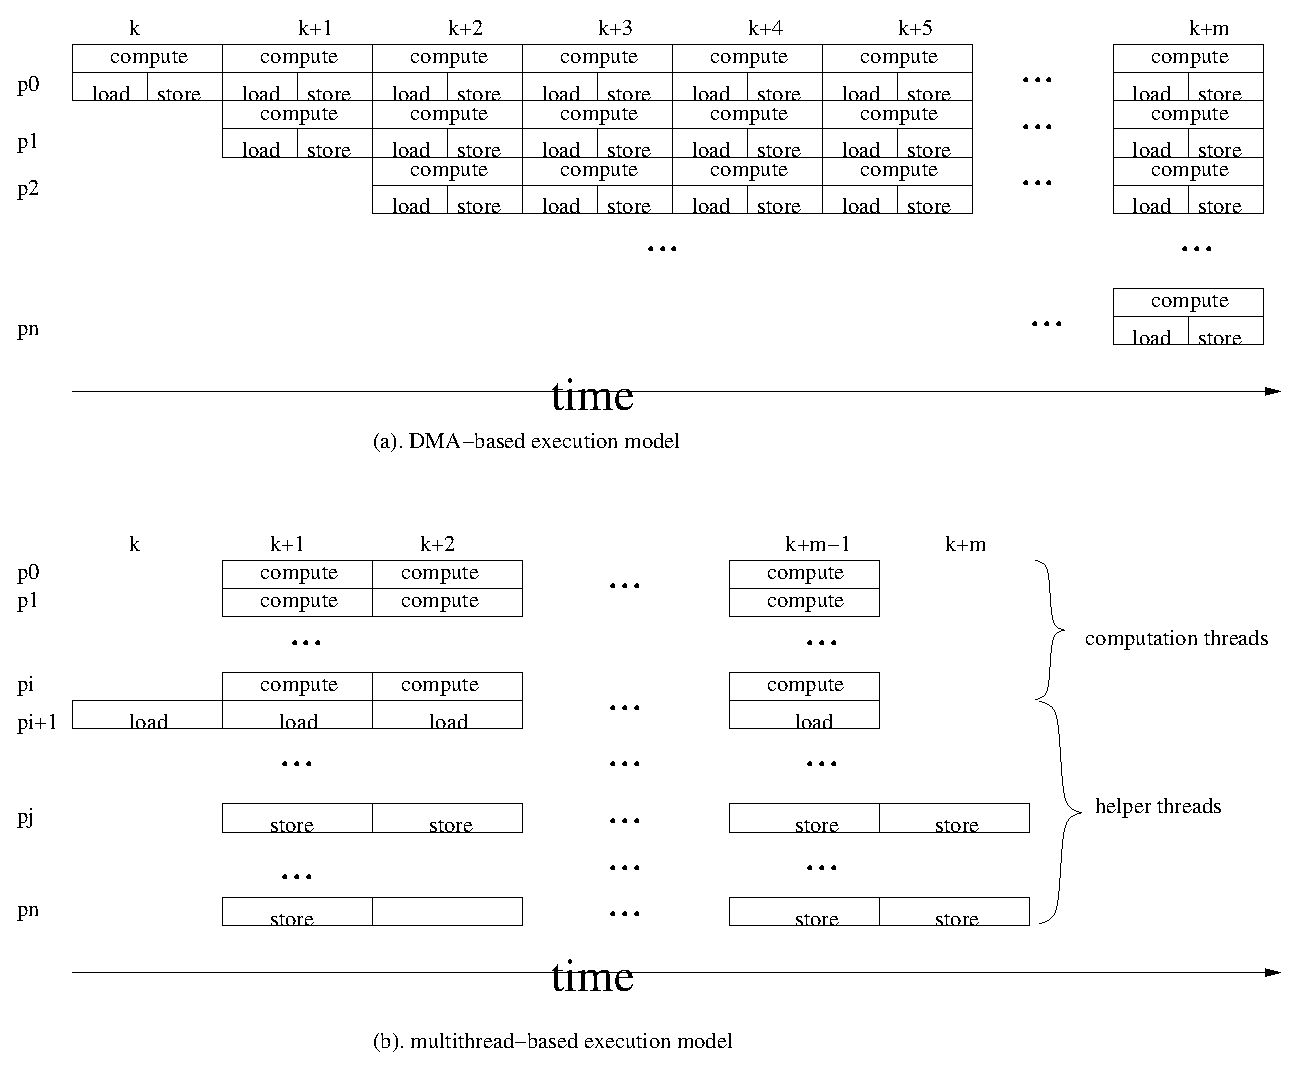
\includegraphics[scale=0.8]{Img/Chap_Algorithm/tolerance_model}\\
	\bicaption{(a). 异步传输的渗透执行模型;(b). 多线程渗透执行模型}{(a). Asynchronous  based percolation; (b). Multithreading based percolation}\label{fig:percolation_method}
	\vspace{-0.5cm}
\end{figure}


\section{组合优化-高性能动态规划算法}\label{sec:PM_dp}

本节介绍对经典组合优化求解算法动态规划的基于渗透模型的并行算法设计和优化。首先给出动态规划算法的基本介绍和重点研究的一类动态规划算法。然后,基于渗透模型的流水线算法实现框架,描述并行动态规划算法。进一步,基于渗透模型的内存层次结构模型,证明了并行算法的最有访存复杂性。最后,在IBM Cyclops64众核处理器结构上进行了实验分析。

\subsection{动态规划算法介绍}
动态规划是求解离散优化问题的一种通用技术,广泛应用于调度问题、仓库管理、自动控制、VLSI设计、交通运输和生物信息学中\citep{dp-book,parallelcomputing-book},其基本思想是将优化问题表达为一
系列的决策过程(求最大或者最小),即形式上表现为一
个决策过程的递归关系式\citep{dp-principle}。设问题{\it r}分解成{\it t}个子问题:$x_{1}, x_{2}, ..., x_{t}$,问题{\it
	r}的解$f(r)$可以表示为:
\begin{equation}\label{op_eq}
r=g(f(x_{1}), f(x_{2}), ..., f(x_{t})
\end{equation}
其中{\it
	g}称为组合函数,它依赖于问题本来的性质。对于优化问题,$g$常常为取最大值或最小值。当$g$取最大值或最小值时,把此方法
称为动态规划法。

求解动态规划的过程通常是填充动态规划矩阵,矩阵中的每一项对应一个子问题,它们的依赖关系根据问题的分解和组合规则确定:如果一
个问题$P$分解成子问题$P_{1}, P_{2}, ..., P_{k}$,问题$P$对应的项的解依赖于$P_{1}, P_{2}, ...,
P_{k}$对应的项的解。动态规划中的子问题之间的依赖关系可用一个有向图$G(V, E)$来表示,图$G$中的一个结点$v_{i}$表示一个子问题,结点$v_{i}$
到
$v_{j}$的边$e_{i,j}$表示结点$v_{i}$表示的子问题的解用于计算$v_{j}$代表的子问题的解。如果有向图无环,图中的结点可以组织成
多级形式,使得第$i$级$level_{i}$的结点的解依赖于其前面一个或者多个级上结点的解。如果任意一级$level_{i}$上的问题的解仅依
赖于$level_{i+1}$上的子问题的解,称之为连续(Serial)动态规划方程,否则如果依赖前面多级子问题的解,称之为非连续的(Nonserial)。
考虑递归方程式,如果一个优化方程中只有一个递归项,称之为一维(Monadic)动态规划方程;如果有多个递归项
,则称 为多维(Polyadic)动态规划方程。基于上述的分类规则,动态规划方程分为连续一维、连续多维、非连续一维和非连续多维
四种形式\citep{parallelcomputing-book}。

本书关注最复杂的一种动态规划即非连续多维动态规划算法,经典的应用有随机上下文无关文法分析\citep{cyk-algo,cyk-algo-1,cyk-algo-2}和矩阵连乘\citep{algorithms-book,matrix-chain}问题,作为计算生物学中重要的问题之一的RNA二级结构预测\citep{rna-pred-bmb,rna-dp,rna-science}也以非连续动态规划算法为核心。为了简化问题以集中分析非连续多维动态规划算法的计算依赖关系,本文使用一种抽象的动态关系方程作为优化目标:
\begin{equation}\label{eq:abstract_dp}
m[i,j] = \left\{ \begin{array}{ll} min_{i \le k < j} \{m[i,j], m[i,k]+m[k+1,j]\} & \textrm{$0 \le i < j < n$}
\\
a(i) & \textrm{$i=j$}
\end{array} \right.
\end{equation}
\begin{figure}[!htbp]
	\begin{center}
		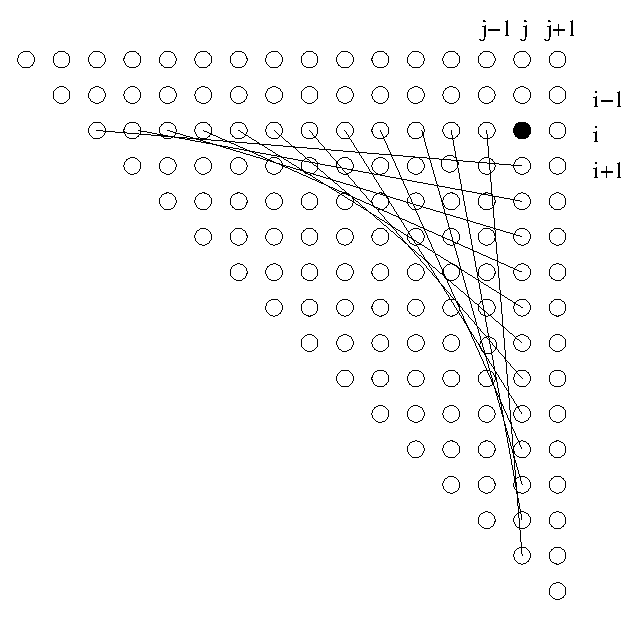
\includegraphics[scale=0.8]{Img/Chap_Algorithm/dp_dependence}
		\caption{非连续多维动态规划算法中的计算依赖关系}\label{fig:dp_dependence}
	\end{center}
\end{figure}

显然,该抽象动态规划方程没有改变非连续多维的计算依赖关系。算法需要计算一个上三角形的动态规划矩阵表,图~\ref{fig:dp_dependence}显示了计算过程中数据依赖关系。矩阵中任何一个
元素的计算依赖于位于同一行和同一列计算完的元素,动态规划矩阵的计算过程能够按行、列和对角线三种方式进行。不失一般性,假设矩阵按列方式存储,这样计算
也按列方式进行。由于该迭代空间是三角形,需要一个中间数组索引按列存储的数组元素(下面算法伪代码中用indx表示)。动态规划方程\ref{eq:abstract_dp}能够
容易地用一个三重循环实现,如算法\ref{algo:standard}所示。
\begin{algorithm}\label{algo:standard}
	{\bf dp\_standard(matrices m, int n)}\\
	for $(j=1; j \leq n; j++)$\\
	\hspace*{1 pc}for $(i=j; i \geq 1; i--)$ \{\\
	\hspace*{2 pc}indxj = indx[j]; \\
	\hspace*{2 pc}ij = i+indxj;\\
	\hspace*{2 pc}$t=m[ij]$;\\
	\hspace*{2 pc}for $(k=i;k<j;k++)$ \\
	\hspace*{3 pc}t=min2(t, m[i+indx[k]]+m[k+1+indxj]) \\
	\hspace*{2 pc}$m[ij]=t$ \\
	\hspace*{1 pc}\}
\end{algorithm}

尽管算法\ref{algo:standard}描述的三重循环和矩阵乘的三重循环类似,但由于非连续多维的计算依赖关系,使得该算法不能利用矩阵乘的通用优化策略。非连续多维动态规划算法的性能低的原因如下:
\begin{itemize}
	\item 不能充分利用存在的局部性。按列顺序的计算过程中,同一列的数据可能保留在Cache中重复使用,但在计算某一列时,依赖的行数据没有重用,而且在实际问题中,
	一行或者一列大小通常超过Cache的大小。按列或者对角线计算也是同样的问题。例如,假设需要计算图中的元素$(i,j)$,需要其同一列的下面的元素$(i+1,j), ..., (j, j)$
	和同一行的元素$(i,i), ..., (i, j-1)$。Cache机制的时间局部性使得列数据可能在Cache中,但依赖的行数据由于Cache替换策略需要重新从内存中读入。
	\item 计算依赖关系限制按列计算从左到右的顺序计算三角形动态规划矩阵,而且在计算某一列时需要从下到上的顺序进行。矩阵中任意一个元素$(i,j)$的计算依赖
	于$O(j-i)$个已经计算的元素,这样,随着计算的进行,依赖关系距离向量是动态变化的。这种动态依赖关系导致:i). 类似优化矩阵乘算法的常规分块策略无效。
	采用优化矩阵乘的分块策略对优化该动态规划算法的性能提高很小,最大只有11\%,大多数情况
	下只有2\%的提高~\citep{TanThesis2008}。ii).  并行任务的负载不平衡。粗粒度并行算法通常对动态规划矩阵在多个处理器之间划分,但随着计算的推进,由于动态的计算依赖关系,静态的
	划分策略很难保证负载平衡,而动态划分引入额外的开销。
	\item 该动态规划矩阵是三角形,不能保证数据存储匹配所有的计算的访存顺序,在某个方向的存储是不连续的。这样,导致了大量的TLB抖动(thrashing)行为的出现,从而大大降低了算法的性能。
\end{itemize}




\subsection{渗透模型的流水算法设计}
非连续多维动态规划算法的运行时特征和计算依赖关系分析表明优化研究需要从以下几个目标:
\begin{itemize}
	\item 在基于Cache/TLB的存储层次结构中,L1
	Cache看作最高一级存储层次,内存为最低一级层次。这里的优化目标是要减少从更低级存储层次读取数据的次数,提高从更高级存储层次读取数据的概率,并且减少TLB不命中
	次数。
	\item 在基于显式存储机制和网络的并行体系结构中,需要开发更多的并行性,以取得隐藏延迟和负载平衡。
	\item
	更多局部性和并行性的获得主要受非连续多维的依赖关系的限制,因此,为了实现前面两个目标,最重要的是对计算依赖关系从算法层进行变换,便于提高程序的局部性和并行性
\end{itemize}
为了解除数据依赖关系导致的并行性受限的问题,\citep{TanThesis2008}提出了一种数据依赖关系变换策略,数据变换算法细节参考文献~\citep{TanThesis2008,TanSC06}。基于变换了数据依赖关系的动态规划方程中,一个子块$A(i,j)$的计算可以用如下公式表示:
\begin{equation}
\label{eq:blocked_eq}
\begin{array}{l}
A(i, j)=\oplus_{k=i}^{j}(A(i,k)\otimes A(k,j))\\
=(\oplus_{k=i+1}^{j-1}(A(i,k)\otimes A(k,j)))\oplus(A(i,i)\otimes A(i,j))\oplus(A(i,j)\otimes A(j,j))
\end{array}
\end{equation}
其中,定义的两个基本矩阵张量操作$\otimes$和$\oplus$,设$A=(a_{ij})_{s\times s}$,$B=(b_{ij})_{s\times
	s}$,$C=(c_{ij})_{s\times s}$
\begin{definition}
	$\forall a_{ij}\in A, b_{ij}\in B, c_{ij}\in C$, $1\le i,j\le s$, if $c_{ij}=min_{k=1}^{n}\{c_{i,j},a_{i,k}+b_{k,j}\}$,
	then $C=A\otimes B$
\end{definition}
\begin{definition}
	$\forall a_{ij}\in A, b_{ij}\in B, c_{ij}\in C$, $1\le i,j\le s$, if $c_{ij}=min\{a_{i,j}, b_{i,j}\}$, then $C=A\oplus B$
\end{definition}

基于渗透模型的多线程系统中,需要“分离”出部分线程用于存储访问。对非连续多维
动态规划问题,只使用2个线程单元用于存储访问的{\em
	helper}线程(后面的性能分析模型中将解释该值的选取)。假设线程个数是$p+2$,其中两个为{\em
	helper}线程,变换数据依赖关系后的动态规划迭代空间规模为$n$。将矩阵划分称若干大小为$2\sqrt{p}$的子块,根据计算依赖关系,任何一块$A(i,j)$依赖于同一行
的其他块$A(i,i...j)$和同一列的块$A(i...j,j)$。对角线上块满足自我闭包属性能够沿对角线方向做细粒度并行计算,但其计算时间只占总时间的一小部分,因此,并行
算法的设计主要考虑其他矩形块的计算。由于块之间的数据依赖关系,按行、列计算不能获得足够的并行,按对角线计算有不能获得好的负载平衡,而且块之间的这种粗粒度
并行需要同时将多个块读入片内存储中,这对片内存储很小的多核体系结构不实用。因此,需要进一步分解计算获得更多的细粒度并行。

一个子块$A(i,j)$($i \ne j$)计算方程\ref{eq:blocked_eq}能够分成两部分。第一部分的计算依赖于同一行同一列的矩形块:
\begin{displaymath}
\oplus_{k=i+1}^{j-1}(A(i,k)\otimes A(k,j))
\end{displaymath}
第二部分的计算依赖于对角线上的三角形块和本身:
\begin{displaymath}
(A(i,i)\otimes A(i,j))\oplus(A(i,j)\otimes A(j,j))
\end{displaymath}
\begin{figure}[htbp]
	\begin{center}
		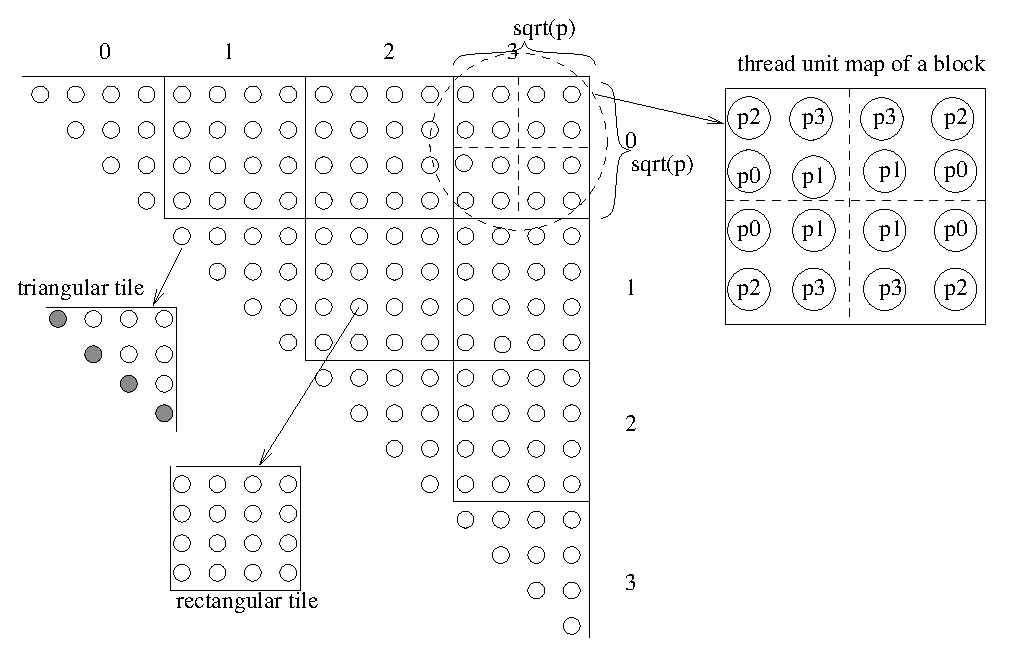
\includegraphics[width=5in,height=2.5in]{Img/Chap_Algorithm/blocked_pdp}
		\caption{细粒度并行算法的数据分块}
		\label{fig:blocked_pdp}
	\end{center}
\end{figure}

图\ref{fig:blocked_pdp}给出了分块的示例,每个块的大小是$4p$,没一条带的第一块是三角形,其他都是矩形。每个块又被划分成大小为$p=\sqrt{p}\times\sqrt{p}$的子块,子块中的元素映射到线程组成的二维网格。更进一步的优化是对矩阵分片,即每个子块的元素都是$x\times y$的片。以计算$A(0,3)$为例,第一部分的计算是$(A(0,1)\otimes A(1,3))\oplus(A(0,2)\otimes A(2,3))$,第二部分的计算是$(A(0,0)\otimes A(0,3))\oplus(A(0,3)\otimes A(3,3))$。第一部分计算表现除了两级并行性:一是$O(j-i-1)$ 个$\oplus$ 操作,二是其中的$\otimes$操作。而第二部分的计算由于两个连续块之间数据依赖关系的限制,并行度相对较底。本节提出的并行算法能够通过调控减少这部分计算。事实上,在计算第二部分的过程中,两个操作$A(i,i)\otimes A(i,j)$, $A(i,j)\otimes A(j,j)$ 都依赖于本身$A(i,j)$,这样把$A(i, i), A(j, j), A(i, j)$合成一个大的三角形矩阵,从而可以沿对角线方向上并行计算。
\begin{figure}[htbp]
	\begin{center}
		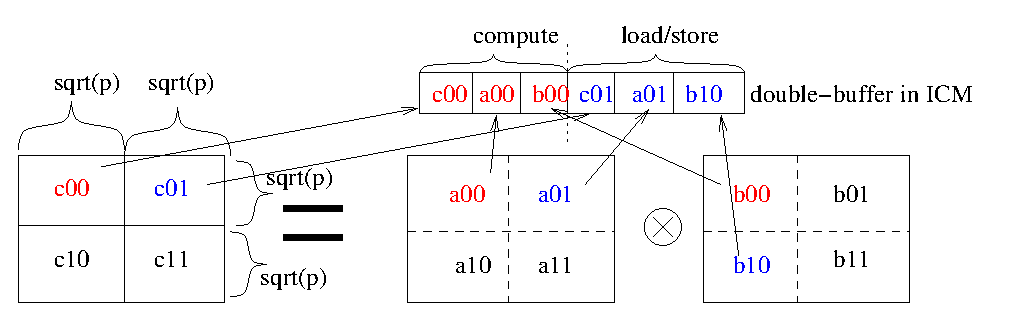
\includegraphics[width=4.5in,height=1.2in]{Img/Chap_Algorithm/sub_block}
		\caption{子块的计算}
		\label{fig:sub_block}
	\end{center}
\end{figure}

第二部分 $\oplus_{k=i+1}^{j-1}(A(i,k)\otimes A(k,j))$的计算中,每个$\otimes$操作能够并行执行。然而,问题是尽管对所有线程单元而言存储访问是一致的,但对不同存储层次的访问是不一致的,因此需要一种策略优化存储访问的开销,以利用片上大规模的线程单元获得高的扩展性。
由于每块大小是$2\sqrt{p}$,把每块又进一步划分成4个大小为$p=\sqrt{p}\times\sqrt{p}$的子块,子块中的每个元素映射到一个线程单元。当执行$\otimes$操作时,所有操作之间没有数据依赖关系,从而可以并行执行。对任何$i+1 \le k \le j-1$,需要计算$A(i,k)\otimes A(k,j)$。为了描述简便,用$C$、$A$和$B$ 分别表示$A(i, j)$、$A(i, k)$和$A(k, j)$。数据依赖关系要求$C$的一个子块的计算需要同一行、列上相应$A$和$B$的子块,这和矩阵乘的计算一样。一个子块的计算需要$(2\sqrt{p})^{3}\times(3+1)=32p\sqrt{p}$ (3 loads and 1 store)存储操作,而且存在数据重用。并行算法把所有线程单元划分成{\em computation}和{\em helper}线程。{\em helper}线程主要用于执行片内和片外存储之间数据移动存取操作,能够和{\em computation}执行计算操作同时进行。为了减少从片外存储读取操作的次数,算法采用double-buffering策略。在片内存储中分配三个double buffer,每个buffer存储其中某个子块的一半。这样,double buffer中,一半存储空间用于计算,一半用于缓存两个存储层次之间的数据交换。计算如图\ref{fig:sub_block}所示,该图演示了计算子块$C(0,0)$的存储映像。为了使{\em computation}和{\em helper}线程能够并行执行,需要满足当{\em computation}线程正在处理当前$C$的一个子块时,{\em helper}线程load/store用于计算$C$的下一个不同子块的数据。为了获得数据重用,$C$的四个子块的计算能够以流水的形式进行,流水过程包括8个并行操作。算法\ref{algo:psteps}描述了计算一个块的并行流水实现,每个操作步后需要一个同步操作以保证当前操作的load/store已经结束。

\begin{algorithm}\label{algo:psteps}
	{\bf ParllelSteps}\\
	startup: LOAD $C00$, $A00$, $B00$; \\
	step 1: COMPUTE $C00$; LOAD $A01$, $B10$;\\
	step 2: COMPUTE $C00$; LOAD $C01$, $B01$;\\
	step 3: COMPUTE $C01$; LOAD $B11$; STORE $C00$;\\
	step 4: COMPUTE $C01$; LOAD $C11$, $A10$;\\
	step 5: COMPUTE $C11$; LOAD $A11$; STORE $C01$;\\
	step 6: COMPUTE $C11$; LOAD $C10$, $B00$;\\
	step 7: COMPUTE $C10$; LOAD $B10$; STORE $C11$;\\
	step 8: COMPUTE $C10$; \\
	end: STORE $C10$;
\end{algorithm}

算法\ref{algo:psteps}需要4个对块$C$的load/stores操作,4个对$A$的load操作和6个对$B$的load操作,因此,计算块$C$需要$18p$个存储操作。尽管算法不能保证存储操作次数是最少的,但算法利用了计算和存储访问之间的并行,通过多线程隐藏了片外存储访问。而一个块$A(i,j)$的计算需要$O(j-i-1)$个$\otimes$操作,注意到算法中的{\em step 8},此时可以用一个{\em helper}
线程读入下一个$\otimes$操作需要的$C00$, $A00$, $B00$,这样,$O(j-i-1)$个$\otimes$操作也形成了流水形式。

如前所述,分片是提高局部性和控制通信粒度的有效策略,这里算法中的通信可以指访问片外存储操作。因此和优化Cache无关算法类似,动态规划矩阵分块对象是分片后的
矩阵。如图\ref{fig:blocked_pdp}所示,这里只考虑正方形片即片参数满足$x=y$。


\subsection{数据流体系结构中显式内存层次的优化}
渗透模型并行算法在IBM Cyclops64上实现并对最优分块因子进行了探索。IBM Cyclops64(C64)芯片是为IBM BlueGene/C千万亿次(PetaFlops)而设计的大规模多核结构,由于本研究的大量实验是在
该平台测试的,这里给出其体系结构的描述。如图\ref{fig:c64node}所示,一个C64芯片包含了80个处理器,每个处理器有两个线程单元(thread unit, TU),即一个芯片上集成了160个64位RISC处理核,5个处理器共享一个指令Cache,取代数据Cache的是分别配置成多个物理上局部的scratchpad
memory(SP)和所有处理单元共享的一致性存储访问的global
memory(GM)。一个芯片上还集成了4个DDR存储控制器以访问片外更多容量的DRAM。芯片内部所有处理单元之间通过crossbar网络互联,其每个端口的带宽达到384GB/s。

\begin{figure}[htbp]
	\centering
	% Requires \usepackage{graphicx}
	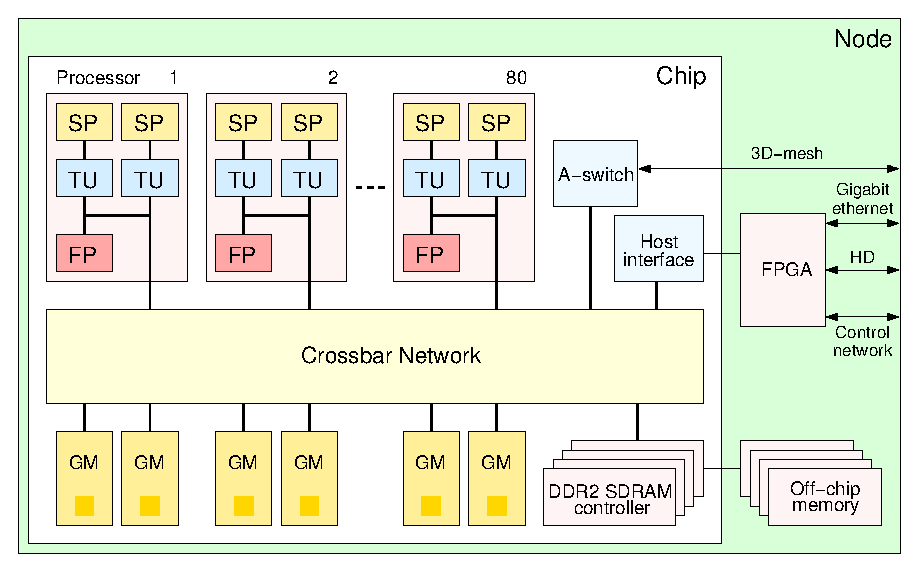
\includegraphics[width=5in,height=2.2in]{Img/Chap_Algorithm/c64node}\\
	\caption{IBM Cyclops64芯片结构}\label{fig:c64node}
\end{figure}
\begin{figure}[htbp]
	\centering
	% Requires \usepackage{graphicx}
	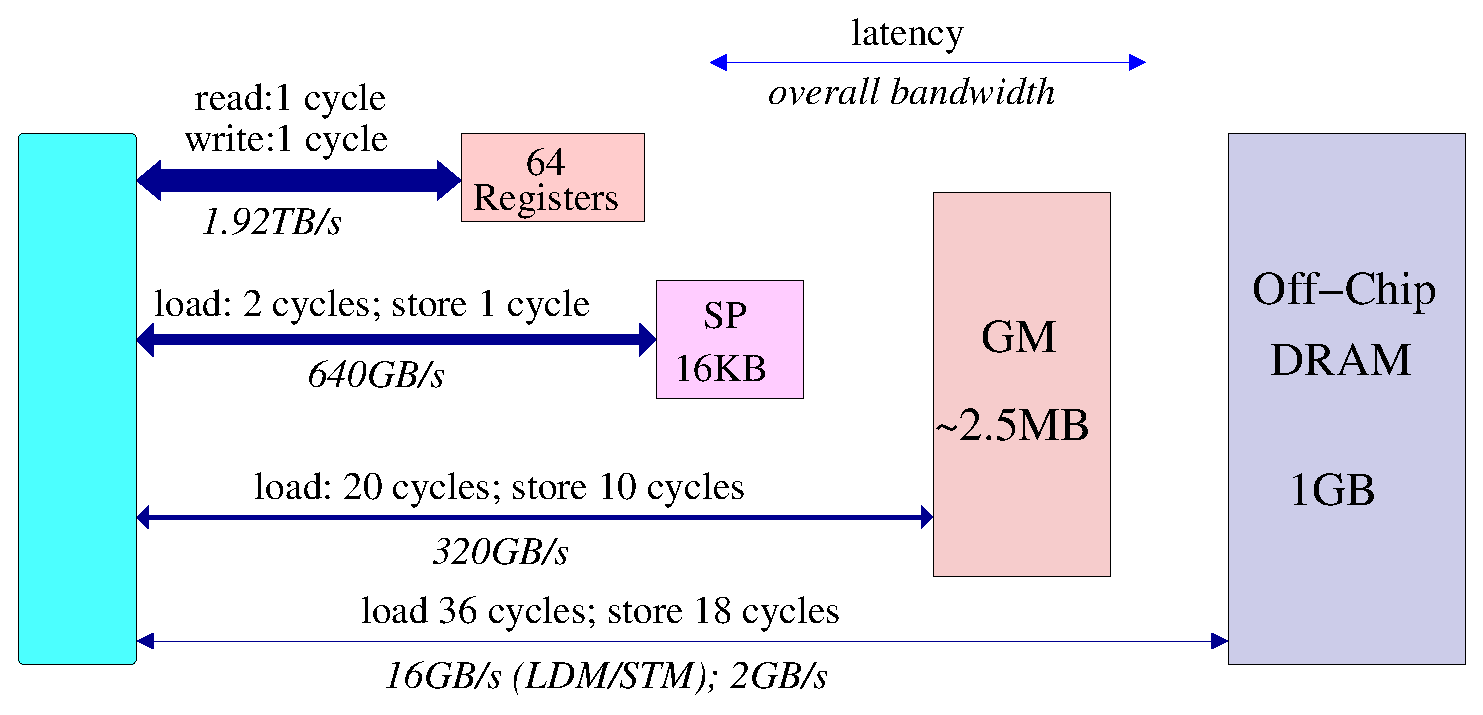
\includegraphics[width=5in,height=2in]{Img/Chap_Algorithm/c64-memory}\\
	\caption{IBM Cyclops64存储层次结构}\label{fig:c64-memory}
\end{figure}
总之,C64芯片体系结构有以下几个突出的特点:
\begin{itemize}
	\item 大规模处理单元、高速嵌入式存储和通信硬件集成到一个芯片上
	\item 支持大规模硬件多线程的有效执行
	\item 不支持虚拟存储管理,而是显式的三级存储层次:Scratchpad memory、on-chip SRAM和off-chip DRAM,
	所有的存储空间为所有的处理单元共享。片上SRAM的一部分配置成scratchpad
	memory,线程单元通过专用的数据通路快速访问自己局部的SP,访问其他线程单元局部的SP需要通过片上网络。其它on-chip
	memory即GM为所有线程单元
	共享并具有一致性存储访问性质,一个线程单元访问另外一个线程单元的SP和GM都需要通过片上crossbar网络。4个片内存储控制可以连接4个片外的大容量存储器,
	也配置成所有处理单元共享并具有一致性访问特点。当前的C64结构中片外DRAM是1GB。图\ref{fig:c64-memory}显示了该存储层次结构的延迟和带宽差异。
	\item 硬件支持barrier和细粒度同步操作
\end{itemize}

由于流水块操作$\otimes$是并行算法的主要计算部分,为了简化模型,
这里只考虑所有块操作$\otimes$的时间。基本的块操作$\otimes$由8个并行步骤组成。假设动态规划迭代空间大小为$n$,分片参数用$x$表示,线程个数用$p$表示。分片后
的迭代空间大小为$m=\frac{n}{x}$,然后对分片后的动态规划矩阵分块,每块大小为$4p=2\sqrt{p}\times
2\sqrt{p}$。这样,如果以块为单元,动态规划矩阵有$m'=\frac{m}{2\sqrt{p}}$行条带,一个行条带$i$有$m'-i$块。根据动态规划依赖关系,行条带$i$上的任何块
$A(i,j),(i\le
j<m'-i$的计算需要$j-i-1$个块操作$\otimes$。用符号$I_{\otimes}$表示整个计算过程所需要的块操作$\otimes$的个数:
\begin{displaymath}
I_{\otimes} = \sum_{i=1}^{m'-2}\sum_{j=i+1}^{m'-i-1}j %= \frac{m'(m'-1)(m'-2)}{3}
\end{displaymath}
因为$m=\frac{n}{x}$,代入上面的方程有:
\begin{equation}\label{eq:iters}
I_{\otimes} = \frac{1}{24}[\frac{n^{3}}{x^{3}p^{\frac{3}{2}}}-6\frac{n^{2}}{x^{2}p}+8\frac{n}{x\sqrt{p}}]
\end{equation}


\subsubsection{存储访问复杂性}
该并行算法的设计基于渗透模型,该模型和out-of-core模型类似,注意到out-of-core模型中用I/O复杂性衡量算法。在本研究中的大规模多核平台具有显式存储层次结构,
如图\ref{fig:c64-memory}所示,把最靠近硬件线程单元的SPM作为一级存储,片内SRAM作为二级存储,片外DRAM作为三级存储。由于SPM主要用于存放线程的状态和
栈等私有数据,一般不用于应用程序数据交换。这样,按照延迟容忍模型的规范,片内SRAM用于ICLM,片外DRAM用于OCM。这里的存储访问复杂性(memory-traffic
complexity)定义为远小于问题规模的片内SRAM和大于问题规模的片外DRAM之间存储访问的次数。从而,有如下引理:
\begin{lemma}\label{lemma:memory_complexity}
	采用分片后的并行流水算法\ref{algo:psteps},分片参数是$x$。其存储访问复杂性(memory-traffic complexity)减少了$x$倍,其中
	$x=O(\sqrt{C})$,$C$是片内SRAM大小。
\end{lemma}

\begin{proof}
	没有采用分片的并行算法,非流水和流水两种形式的存储访问复杂性分别为:
	\begin{displaymath}
	M_{non-pipeline} = I_{\otimes}\times 32p\sqrt{p} = O(n^{3})
	\end{displaymath}
	\begin{displaymath}
	M_{pipeline} = I_{\otimes}\times 18p = O(\frac{n^{3}}{\sqrt{p}})
	\end{displaymath}
	当对矩阵分片后,每个$\otimes$操作的元素是以大小为$x\times
	x$的片为单位。每个$\otimes$操作产生$x^{2}$次存储访问,因此一个块$\otimes$操作的存储访问次数是$18px^{2}$。考虑整个算法的块操作次数$I_{\otimes}$,得到分片后
	并行流水算法的存储访问复杂性为:
	\begin{displaymath}
	\begin{array}{ll}
	M_{tile} = I_{\otimes}\times 18p \\
	\hspace*{3pc}= \frac{1}{24}[\frac{n^{3}}{x^{3}p^{\frac{3}{2}}}-6\frac{n^{2}}{x^{2}p}+8\frac{n}{x\sqrt{p}}]\times 18p=O(\frac{n^{3}}{x\sqrt{p}})
	\end{array}
	\end{displaymath}
	证毕。
\end{proof}
引理\label{lemma:memory_complexity}给出了算法存储访问复杂性的上界,由于算法的基本操作$\otimes$和矩阵乘的计算行为一样,而且以前的研究证明了其存储访问
复杂性的下界为$\Omega(\frac{n^{3}}{x\sqrt{p}})$\citep{layout-tpds03},从而有下面关于在多核结构上的并行流水动态规划算法的存储访问复杂性定理:
\begin{theorem}
	分片的并行流水算法的存储访问复杂性是近似最优的。
\end{theorem}
存储访问复杂性的概念衡量了一个算法在通用体系结构上类似的存储访问次数。然而,注意到大规模多核结构中,“分离”出的{\em
	helper}线程专门用于存储访问以实现计算和片外存储访问的重叠,而且在有限的带宽内,{\em
	helper}的片外存储访问也可以并行。因此算法的设计要权衡需要多少个“分离”的{\em
	helper}线程。这里提出另外一个概念--存储访问效率(memory-traffic efficiency),定义为存储访问减少量和{\em
	helper}线程个数的比值。本节提出的并行流水算法使用了两个{\em
	helper}线程,其中一个用于load操作,另一个用于store操作,则4个store操作能够完全被重叠,导致时间的减少量为$4/18$,因此存储访问效率是11\%。但注意到
算法\ref{algo:psteps}中每个并行步最多只需要两个片外存储访问,如果不静态限定{\em helper}线程的操作,而是在某个{\em
	helper}线程空闲时去执行store操作,则4个load和4个store操作能够被隐藏,从而时间减少量为$8/18$,存储访问效率为22\%。如果使用3个{\em
	helper}线程,所有的片外存储访问操作能够并行执行,时间减少量为$10/18$,但存储访问效率是19\%。可以看出,存储访问效率取决于存储访问中的并行性,而且在实际
的平台上其并行性受带宽的限制,所以,使用更多的{\em helper}线程并不意味着高的性能。
\subsubsection{运行时间}
通过分片的并行流水算法分析,并行算法的运行时间受分片参数$x$的影响,本节构建关于最小化运行时间的性能分析模型以确定得到最少运行时间的分片参数$x$。假设
一个标准三重循环实现的动态规划的运行时间为$\alpha$,一次片外存储访问延迟为$\beta$。算法\ref{algo:psteps}的每一个步骤中,一个线程需要执行$\sqrt{p}$个
$\otimes$操作,这样,一个并行步的计算时间为:
\begin{displaymath}
T_{comp} = \alpha\sqrt{p}x^{3}
\end{displaymath}
如前面的分析,两个存储访问能够并行执行,片外存储访问的延迟为:
\begin{displaymath}
T_{tran} = \beta px^{2}
\end{displaymath}
由于{\em computation}线程和{\em
	helper}线程能够并行进行,相应地,片外和片内存储之间的数据传输和计算时间被重叠起来,因此,一个分片的基本操作$\otimes$的运行时间为:
\begin{equation}\label{eq:block_time}
T_{\otimes}=max\{T_{comp}, T_{tran}\}=max\{\alpha\sqrt{p}x^{3},\beta px^{2}\}
\end{equation}
合并方程\ref{eq:iters}和\ref{eq:block_time},得到并行流水算法的运行时间:
\begin{equation}\label{eq:execution}
\begin{array}{ll}
T_{0}(x) = \frac{n}{2x\sqrt{p}}\times2\beta px^{2}+I_{\otimes}\times 8\times T_{\otimes}\\
=n\beta\sqrt{p}x+8\times I_{\otimes}\times max\{\alpha\sqrt{p}x^{3},\beta px^{2}\}\\
=\left\{ \begin{array}{ll} T_{1}(x)=n\beta\sqrt{p}x+8I_{\otimes}\times\beta px^{2} &
\textrm{$x<\frac{\beta\sqrt{p}}{\alpha}$}\\
T_{2}(x)=n\beta\sqrt{p}x+8I_{\otimes}\times\alpha\sqrt{p}x^{3} & \textrm{$x\ge\frac{\beta\sqrt{p}}{\alpha}$}
\end{array} \right.
\end{array}
\end{equation}
对角线上的三角形块是自我闭包的,其运行时间为:
\begin{equation}\label{eq:tri}
T_{3}(x)=(\sum_{i=1}^{m'}i\times\sum_{j=1}^{4\sqrt{p}}+m'\sum_{j=1}^{2\sqrt{p}})x^{3}\alpha =n\alpha
px^{2}+\frac{n^{2}\alpha(4\sqrt{p}+1)}{4}x
\end{equation}
因此,选择最优的分片参数即为解下面的优化问题:
\begin{equation}\label{eq:all}
\begin{array}{ll}
\mathcal{P}:Minimize\hspace*{1pc}T(x)=T_{0}(x)+T_{3}(x) \\
\hspace*{4pc} s.t. \hspace*{1pc}\frac{\beta\sqrt{p}}{\alpha}\le x<min\{\sqrt{\frac{C}{48p}},\frac{n}{4\sqrt{p}}\}
\end{array}
\end{equation}
该优化问题的目标是求解最优的分片参数$x$以最小化函数$T(x)$。为了解该非线性优化问题,需要先给出并证明两个推论。注意到目标函数满足下列属性:
\begin{displaymath}
\begin{array}{ll}
T_{1}(x) \ge T_{2}(x) & \textrm{$x\le\frac{\beta\sqrt{p}}{\alpha}$}
\end{array}
\end{displaymath}
\begin{displaymath}
\begin{array}{ll}
T_{1}(x) = T_{2}(x) & \textrm{$x=\frac{\beta\sqrt{p}}{\alpha}$}
\end{array}
\end{displaymath}
\begin{displaymath}
\begin{array}{ll}
T_{1}(x) \le T_{2}(x) & \textrm{$x\ge\frac{\beta\sqrt{p}}{\alpha}$}
\end{array}
\end{displaymath}
这样,优化问题转化为:
\begin{equation}\label{eq:opt}
\begin{array}{ll}
\mathcal{P_{0}}:\hspace*{1pc}Minimize\hspace*{1pc}T_{0}(x) = 8\times min\{max\{T_{1}(x), T_{2}(x)\}\} \\
\hspace*{3pc}s.t.\hspace*{1pc}\textrm{$x=O(\sqrt{C})$}
\end{array}
\end{equation}
在并行流水算法中,片内SRAM至少有6个大小为$p$个片的存储块用于数据交换实现double-buffering,其元素数据类型是{\em double},从而得到下面的限制条件:
\begin{equation}\label{eq:c1}
x < \sqrt{\frac{C}{48p}}
\vspace{-0.225cm}
\end{equation}
另外,由于$I_{\otimes}>0$,推导出第二个限制条件:
\begin{equation}\label{eq:c2}
x < \frac{n}{4\sqrt{p}}
\end{equation}
综上,结合方程\ref{eq:iters}、\ref{eq:opt}、 \ref{eq:c1}和 \ref{eq:c2},非线性优化问题表示如下:
\begin{equation}\label{eq:opt_inst}
\begin{array}{ll}
\mathcal{P'}:\hspace*{1pc}Minimize\hspace*{1pc}T_{0}(x) \\
=\frac{1}{24}\left\{ \begin{array}{ll} T_{1}(x)= \frac{n^{3}\beta}{\sqrt{p}x}+9n\beta\sqrt{p}x-6n^{2}\beta &
\textrm{$x\le\frac{\beta\sqrt{p}}{\alpha}$}\\
T_{2}(x)= 8n\alpha x^{2}+(n\beta\sqrt{p}-\frac{6n^{2}\alpha}{\sqrt{p}})x+\frac{n^{3}\alpha}{p} &
\textrm{$x\ge\frac{\beta\sqrt{p}}{\alpha}$}
\end{array} \right. \\
\hspace*{3pc}s.t.\hspace*{1pc}\textrm{$x<\sqrt{\frac{C}{48p}}$} \\
\hspace*{4pc}\hspace*{1pc}\textrm{$x<\frac{n}{4\sqrt{p}}$}
\end{array}
\end{equation}
最优问题的解用$x^{*}$表示,现在证明推论\ref{cor:solution1}。
\begin{corollary}\label{cor:solution1}
	给定问题规模$n$和片内SRAM大小$C$,优化问题$\mathcal{P"}$的最优解$x^{*}$为:
	\begin{displaymath}
	x^{*}=\left\{\begin{array}{ll} \lfloor\frac{n}{4\sqrt{p}}\rfloor-const & \textrm{$n\le\sqrt{\frac{C}{3}}$} \\
	\lfloor\sqrt{\frac{C}{48p}}\rfloor-const & \textrm{$n\ge\sqrt{\frac{C}{3}}$}
	\end{array}\right.
	\end{displaymath}
	其中$const$是一个使$x^{*}>0$的常数。
\end{corollary}
\begin{proof}:
	$T_{1}(x)$和$T_{2}(x)$的解分别用$x_{1}^{*}$和 $x_{2}^{*}$表示,它们满足如下关系:
	\begin{displaymath}
	x_{1}^{*}=\frac{n}{3\sqrt{p}} \hspace*{2pc}x_{2}^{*}=\frac{6n\alpha-p\beta}{16\alpha\sqrt{p}}
	\end{displaymath}
	设$x_{mid}^{*}=\frac{\beta\sqrt{p}}{\alpha}$把优化问题的解空间划分成两部分:$(0,
	x_{mid}^{*}]$和$[x_{mid}^{*}, min\{\sqrt{\frac{C}{48p}},\frac{n}{4\sqrt{p}}\})$。显然,
	$x_{1}^{*}>\frac{n}{4\sqrt{p}}$和$x_{2}^{*}>\frac{n}{4\sqrt{p}}$表明$x_{1}^{*}$和$x_{2}^{*}$ 已经超出了解空间,在解空间中,位于$x_{1}^{*}$和$x_{2}^{*}$左边时,$T_{1}(x)$和$T_{2}(x)$ 是递减的且在$min\{\sqrt{\frac{C}{48p}},\frac{n}{4\sqrt{p}}\}-const$时达到最小值。
\end{proof}
\begin{corollary}\label{cor:solution2}
	给定问题规模$n$而且$2<p<\frac{\alpha}{\beta}min\{\sqrt{\frac{C}{48}},\frac{n}{4}\}$,优化问题$\mathcal{P}$的解为
	$x^{*}=\frac{\beta\sqrt{p}}{\alpha}$ 
\end{corollary}
\begin{proof}
	设$a=(8n\alpha+n\alpha p)$,$b=(n\beta\sqrt{p}-\frac{6n^{2}\alpha}{\sqrt{p}}+\frac{n^{2}\alpha(4\sqrt{p}+1)}
	{4})$,当$x^{*}=\frac{-b}{2a}$,$T(x)$取得全局最小值。然而,解空间的区间为[$\frac{\beta\sqrt{p}}{\alpha}$, $min\{\sqrt{\frac{C}{48p}},\frac{n}{4\sqrt{p}}$\})。假设$x^{*}>
	\frac{\beta\sqrt{p}}{\alpha}$,有:
	\begin{equation}\label{eq:theorem2}
	n<\frac{4\beta p(2p+17)}{24\alpha-\alpha\sqrt{p}(4\sqrt{p}+1)}
	\end{equation}
	根据方程\ref{eq:theorem2},$n>0$ 当且仅当 $p\le 2$。也就使说,$p>2$而且$x^{*}<\frac{\beta\sqrt{p}}
	{\alpha}$。一元二次方程的属性表明当 $x>x^{*}$时,$T(x)$递增。优化问题$\mathcal{P}$的解为$\frac{\beta\sqrt{p}}{\alpha}$
\end{proof}
根据推论\ref{cor:solution1}和\ref{cor:solution2},得到下面求解最优分片问题中分片参数的定理:
\begin{theorem}\label{thm:solution}
	分片并行流水动态规划算法的最优分片参数由如下规则确定:
	如果$2<p<\frac{\alpha}{\beta}min\{\sqrt{\frac{C}{48}},\frac{n}{4}\}$,
	$x^{*}=\frac{\beta\sqrt{p}}{\alpha}$;
	否则,
	\begin{displaymath}
	x^{*}=\left\{\begin{array}{ll} \lfloor\frac{n}{4\sqrt{p}}\rfloor-const & \textrm{$n\le\sqrt{\frac{C}{3}}$} \\
	\lfloor\sqrt{\frac{C}{48p}}\rfloor-const & \textrm{$n\ge\sqrt{\frac{C}{3}}$}
	\end{array}\right.
	\end{displaymath}
\end{theorem}
\begin{figure}[!htbp]
	\begin{center}
		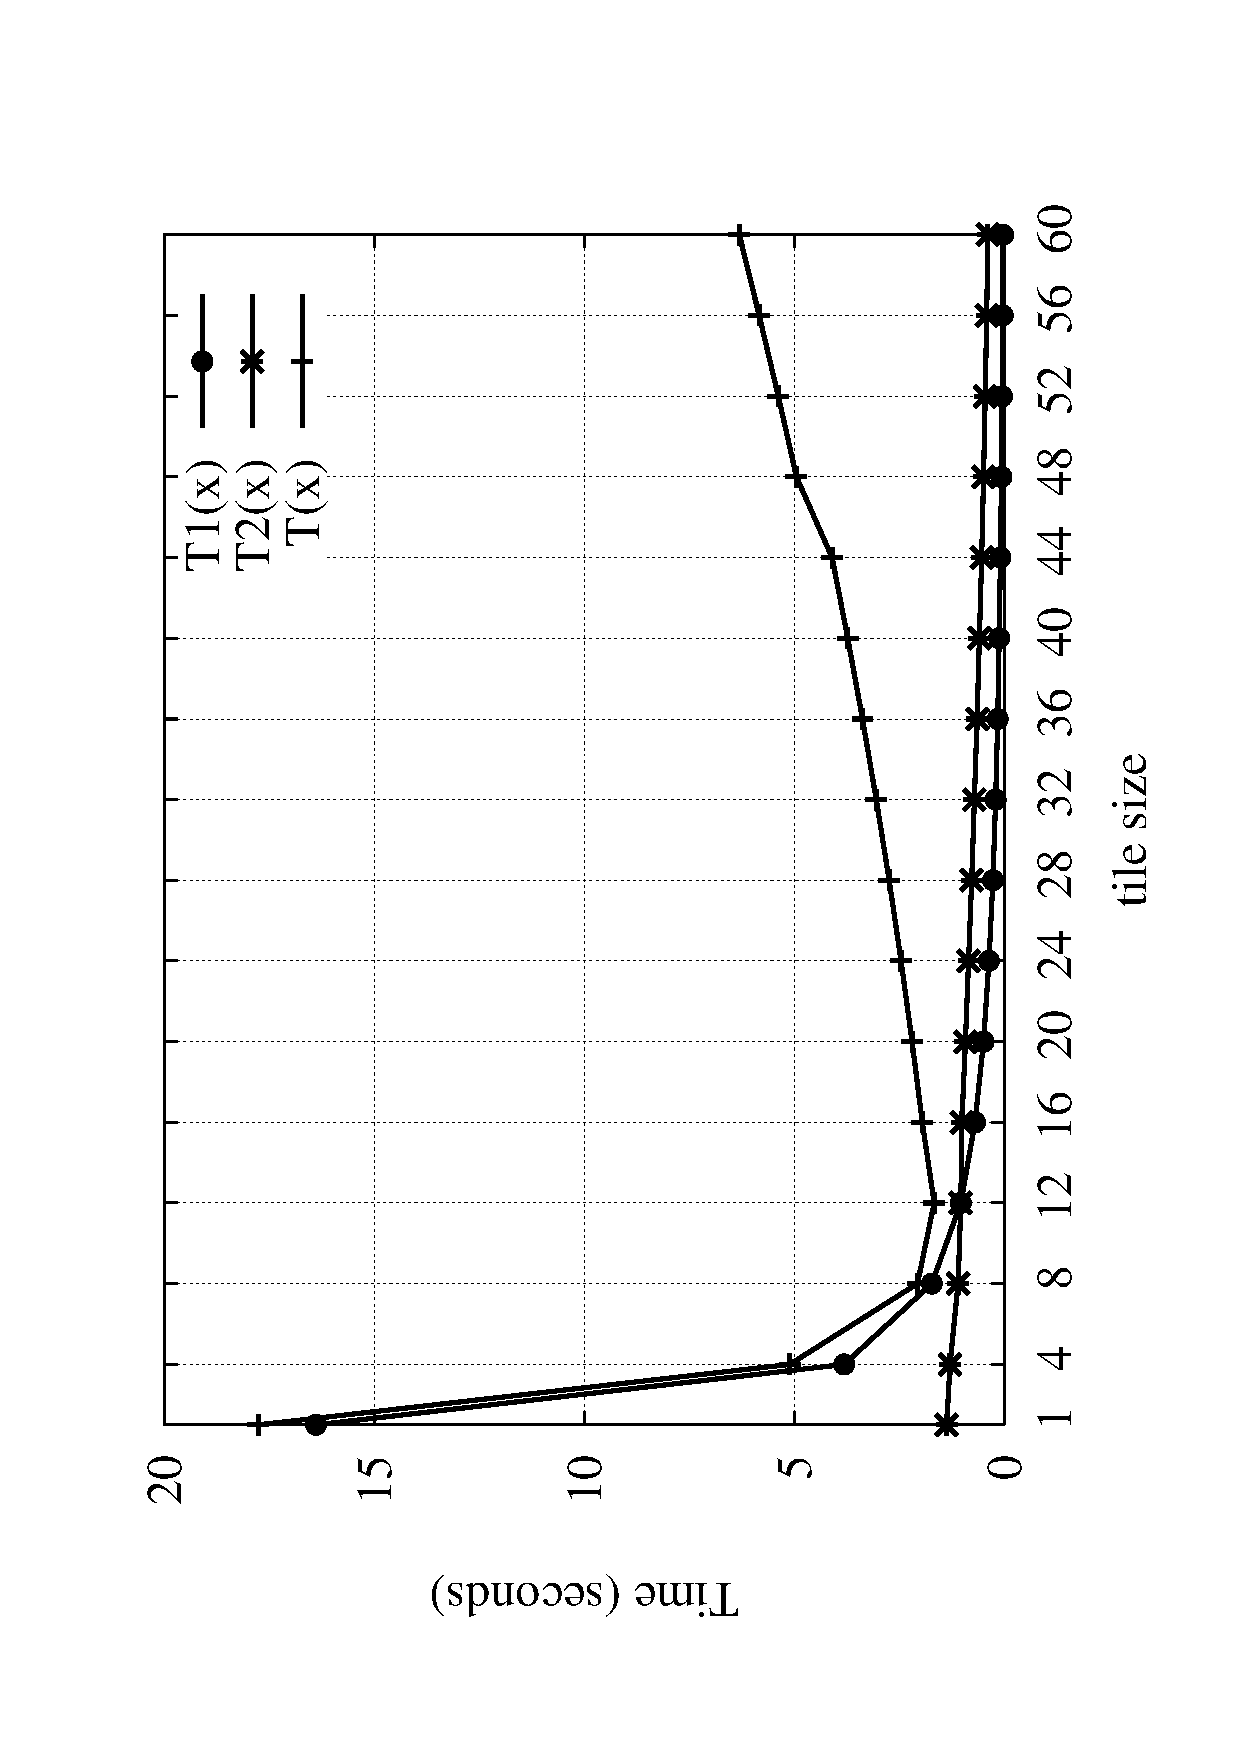
\includegraphics[scale=0.6]{Img/Chap_Algorithm/model}
		\caption{最优分片的理论分析}
		\label{fig:model}
	\end{center}
\end{figure}

图\ref{fig:model}给出了问题规模是$n=1024$在$p=16$时的最优解,根据定理\ref{thm:solution}在$p=16$,$n=1024$的最优解。其中  $x_{mid}^{*}=12$
$min\{\sqrt{\frac{C}{48p}},\frac{n}{4\sqrt{p}}\}=64$, $x^{*}=12$。
$T_{0}(x)$的解说明$x$越大越好,然而增加$x$的值导致计算并行度底的三角形部分的计算增加。事实上,前述优化问题解能够解释并行算法的扩展性。$x_{mid}^{*}$把解空间划分成两部分。当最优解落入左边区间时,即$\frac{n}{p}<\frac{\beta}{\alpha}$,说明当线程数量超过一定值时,程序的执行时间由存储数据传输决定。推论\ref{cor:solution1}证明了最优解位于$x_{mid}^{*}$的右边,这说明并行算法的扩展性主要取决与计算操作数量,而不是存储访问延迟。因此,本研究提出的并行流水算法在具有显式存储的大规模多核体系结构上有较好的扩展性。

\begin{table}
	\begin{center}
		\caption{不同问题规模下的运行时间(效率)。单位: 秒(seconds)} \label{tab:exe_time}
		\begin{tabular}{|l|l|l|l|l|l|}
			\hline
			\#threads & 256 & 512 & 1024 & 2048 & 4096 \\\hline
			serial & 1.40 & 11.28 & 90.43 & 226.54 & 1738.88\\\hline
			4 & 0.36 & 2.46 & 17.94 & 42.72 & 275.82\\\hline
			16 & 0.16 & 1.01 & 6.99 & 15.75 & 106.28\\\hline
			64 & 0.12 & 0.62 & 4.57 & 7.57 & 44.06\\\hline
		\end{tabular}
	\end{center}
\end{table}
表\ref{tab:exe_time}总结了串行程序和并行程序的运行时间,数据显示并行算法获得了近似线性的加速比。算法\ref{algo:psteps}的并行流水计算策略提高数据重用,减少了片外存储的访问次数,从而大大降低了存储访问的开销。通过以前的算法理论分析,片外存储访问数量能够被减少近似3倍,但注意到算法采用了分片技术进一步提高程序运行时的局部性,所以性能提高要略大于3倍。该并行流水算法通过增加数据重用而优化了访问片外存储的带宽。同时,IBM Cyclops64也支持同时多个存储load/store操作的指令,如LDM/STM指令由4个LDD/STD(load/store double word)实现,因此,如果程序能够使用这些指令,则理想情况下带宽利用可以增加将近4倍。




\section{大数据分析-高性能图遍历算法}\label{sec:PM_graph}

本节介绍对大数据分析应用中的图计算问题的基于渗透模型的并行算法设计和优化。首先给出大规模网络分析算法介度中心(betweenness centrality)的图计算算法。然后,基于渗透模型的流水线算法实现框架,描述并行介度中心图遍历算法。进一步,利用数据流体系结构中硬件同步机制的支持优化图计算问题。

\subsection{图遍历算法介绍}
大规模网络分析方法应用于许多重要的应用中如社会网络分析(亲朋关系、组织结构和反恐)、WWW因特网(网络拓扑)、交通运输网络、家谱关系和生物信息学
(蛋白质相互作用网络、性/AIDS网络和食物网络)\citep{network-app-social-Freeman,network-app-social-url,network-cs-acm,network-cs-connections,network-app-web,network-app-internet,network-app-bioinformatics,network-app-nature,network-app-recomb,network-app-aids}。在大多数应用中,图的抽象和算法经常用于描述和解释问题的本质\citep{network-app,network-app-sci}。基于图论的网络分析能够从
真实数据构建的大规模图来抽取有意义的信息,如识别反恐网络中关键人物、蛋白质网络中起主要调控作用的蛋白等。

构建合适的模型模拟复杂的真实世界网络本身就是一个
相当重要而活跃的研究课题\citep{network-model-nas, network-model-globcomm,network-model-rmat}。在过去的几十年中,随机网络(random
networks)\citep{network-model-nas}模型一直是大规模网络分析的主要研究工具。构建一个图时,每个顶点的度$k$服从某个概率分布$P(k)$。在随机图中,由于每个顶点的边数随机选择,
大多数顶点的度几乎一样。然而,最近的大量研究表明许多复杂的网络系统显示出有组织的结构。人们又提出了Scale-Free(SF)网络模型\citep{network-sf-math,network-sf-phy}。SF网络中的顶点的度服从幂律(power-law)分布\citep{network-power-law},即:
\begin{equation}\label{eq:power_law}
P(k)\sim k^{-\gamma}
\end{equation}
和SF网络模型匹配的网络分析应用有WWW因特网、蛋白质相互作用网络和性/AIDS网络等。与随机网络中度的均匀分布不同,SF网络中绝大多数顶点只有很少的连接,只有
少数几个顶点有许多的连接。

分析大规模网络的一个最重要的工具是图的向心性指标(centrality
index)\citep{network-centrality}。社会网络分析中,顶点的向心性用来给所有的参与者分级和区别最主要的参与者;在蛋白质网络中,蛋白质的向心性识别具有高度互联的一组蛋白质,这些蛋白质
在调控相互作用中扮演主要角色。到目前为止,已经有多个向心性指标用于分析网络特征,其中最重要的一个就是
介度中心(betweenness centrality)\citep{network-bc}。

用图$G=(V,E)$表示一个网络结构,其中$V$是顶点集合,$E$是边集合。顶点和边的数量
分别用$n$和$m$表示,图可以是有向或者无向的。每一条边赋予一个权值$w(e)$(无权图中$w(e)=1$)。从顶点$s$到$t$的路径用多个有序的二元组
$<u_{i},u_{i+1}>$表示,其中$0\le i\le l, u_{0}=s, u_{t} =
t$,路径的长度$d(s,t)$是该路径上所有边的权值的和。用$\sigma_{st}$表示顶点$s$和$t$之间最小路径的条数,而其中经过另外一个顶点$v$的最小路径条数用
$\sigma_{st}(v)$表示。1977年,Freeman\citep{network-bc}首次提出了介度中心概念。用$\delta_{st}(v)$表示任意顶点的两两依赖性(pairwise
dependency),即顶点$s$到$t$之间的最小路径中经过顶点$v$的条数与总数的比值:
\begin{equation}\label{eq:pairwise_dep}
\delta_{st}(v)=\frac{\sigma_{st}(v)}{\sigma{st}}
\end{equation}
任意一个顶点$v$的介度中心(betweenness centrality)定义如下:
\begin{equation}\label{eq:bet_cent}
BC(v)=\sum_{s\ne v\ne t\in V}\delta_{st}(v)
\end{equation}
介度中心的值度量一个顶点在网络中交互的控制地位,辨别出其中关键的部分。高的介度中心值表明该顶点通过相对较短的最小路径达到其他顶点,即该顶点在连接其他
顶点的路径中是更关键的部分。直接计算所有顶点的介度中心值的算法如下:
\begin{enumerate}
	\item 计算任意顶点对$(s,t)$之间的最小路径长度和数量;
	\item 对每一个顶点$v$,计算所有可能的两两依赖性$\delta_{st}(v)$,然后求和。
\end{enumerate}
通过Floyd-Warshall算法计算所有顶点对之间最小路径算法,该直接计算的时间复杂度是$O(n^{3})$。基于Dijkstra单源最小路径算法和宽度优先搜索(breadth
first search)算法,通过消除计算过程中的冗余计算,Brandes\citep{brandes-bc}提出了一种时间复杂度为$O(mn+n^{2}logn)$的快速算法。

定义从$s$出发的最短路径上一个顶点$v$的前驱集合:
\begin{equation}
P_{s}(v)=\{u\in V: \{u,v\}\in E, d(s,v)=d(s,u)+d(u,v)\}
\end{equation}
为了消除计算所有两两依赖性的冗余部分,增加一个中间变量$\delta_{s}(v)$表示源顶点$s\in V$对其最短路径上某个顶点$v\in
V$的依赖性:
\begin{equation}
\delta_{s}(v)=\sum_{t\in V}\delta_{st}(v)
\end{equation}
Brandes算法较少计算量的最重要观察是$\delta_{s}(v)$满足如下的递归关系:
\begin{equation}\label{eq:delta}
\delta_{s}(v)=\sum_{w:v\in P_{s}(w)}\frac{\sigma_{sv}}{\sigma_{sw}}(1+\delta_{s}(w))
\end{equation}
$\delta_{s}(v)$事实上是$BC(v)$的部分中间结果值,最后,$BC(v)$的计算表示如下:
\begin{equation}\label{eq:BC}
BC(v)=\sum_{s\neq v\in V}\delta_{s}(v)
\end{equation}
和动态规划求解问题类似,计算介度中心算法也明显分为两个连续阶段:向前BFS得到最小路径(后面简称BFS)和向后累加依赖性值(简称回溯)。
\begin{enumerate}
	\item {\bf BFS:}在BFS阶段, 对每一个顶点$s\in
	V$遍历图搜索最小路径,同时保留所有最小路径上的顶点的前驱集合$P_{s}(v)$和经过中间顶点$w$的最小路径的条数$\sigma(w)$。
	\item {\bf 回溯:}对每一个源顶点$s$,使用其最小路径树的信息如经过中间顶点$w$的最短路径条数$\sigma(w)$和前驱集合,根据递归
	式\ref{eq:delta}计算$\delta_{s}(v)$。最后累加所有部分值得到顶点$v$的介度中心值。
\end{enumerate}

尽管图分析算法广泛应用于大量重要的实际问题中,然而由于其相当不规则的计算特征,导致大多数的图算法不同于传统的科学计算,不能够采用常规的优化策略提高
程序运行性能。图算法区别与多数传统科学计算的非规则特点如下:
\begin{itemize}
	\item {\bf
		很少的局部性和数据重用:}真实世界的网络规模巨大,通常有上百万甚至上亿顶点和边。如何设计空间有效的数据结构存储大规模数据表示就是一个极具挑战性的问题,
	并行外部算法设计(out-of-core
	algorithms)已经证明了在一定情况下是一种可行的策略。然而,这种策略要求数据结构是可以划分的,这对大多数规则的科学计算问题相当适合;但模拟真实世界
	网络的图结构由于其高度非结构性而通常不可简单划分。图中每个顶点的度也是分布不均,如本研究中SF图模型。这种非结构性的度分布也导致了程序在存储访问时
	可变的步长和随机性,从而很难在基于Cache存储结构上获得局部性。通常,在一次图遍历的过程中,一个顶点只需要访问一次,这样几乎不存在数据重用。
	\item {\bf
		动态非连续存储访问:}事实上,大多数的图算法中计算操作相对存储访问的比例很低,而且存储访问模式不能够静态地确定。例如,图遍历算法按级访问所有顶点,
	下一级需要访问的顶点是在当前一级遍历时动态确定的。也就是说,存储访问模式是动态数据相关的,这样,常规的体系结构上的预取机制不能有所帮助。而且由于
	两个顶点的邻接关系也是动态随机生成的,导致大量的非连续的存储访问。
	\item {\bf
		细粒度并行性:}遍历图通常按级进行,但级之间存储数据依赖关系,所以不能在级之间实现粗粒度并行。遍历一个顶点的所有邻接点时,可能存在并行访问的
	情况。但相对于大规模并行计算机,这种并行性是细粒度的,特别是对稀疏图如SF图模型。在同一级,如果有多个顶点,遍历这些顶点的邻接点可能可以并行进行,
	但如果两个顶点共享一个邻接点时,需要同步机制保证冲突访问。
\end{itemize}

大多数常规的基于Cache并行计算机体系结构的设计出自程序中具有高度局部性、规则存储访问模式和强调计算操作的粗粒度并行,显然,图算法这些源于非规则的计算行为的特征限制了在目前常规并行体系结构上获得高的加速比和好的可扩展性。


\subsection{渗透模型的流水算法设计}
把BFS阶段访问一个顶点的邻接点的操作称为扩展,当前需要扩展的顶点保存在一个队列中。

\begin{figure}[htbp]
	\begin{center}
		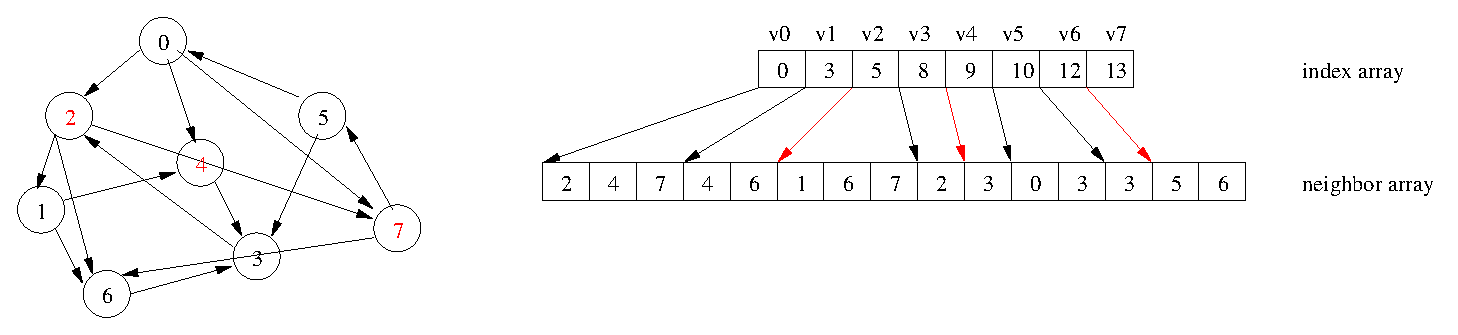
\includegraphics[width=6in,height=1.5in]{Img/Chap_Algorithm/adjacent}
		\caption{邻接数组数据结构}
		\label{fig:adjacent}
	\end{center}
\end{figure}

由于需要分析的图是稀疏图,算法采用存储空间有效的数据结构-邻接数组(adjacent array)来表示稀疏SF图,如图\ref{fig:adjacent}所示。邻接数组由两个数组组成:索引数组(index array)和邻接数组(neighbor array)。索引数组中的第$i$个元素表示顶点$i$的邻接点连续存储在邻接数组中偏移位置。当访问一个顶点的邻接点时,由于其邻接点是连续存储的,当顶点的度较高时,基于Cache体系结构上的预取或者分块技术可能可以优化性能,然而,稀疏SF图中绝大多数顶点的度都很低。两个不同顶点的邻接点的存储可能不是连续的,预取的邻接点可能不是即将要访问的顶点,这样不仅出现预取无效,而且导致大量Cache不命中,从而大大降低了程序的性能。介度中心算法还需要4个数据结构存储BFS树和每个顶点的介度中心值。存储前驱顶点的数据结构和邻接数组一样,表示$d, \sigma, \delta$分别是大小为$n$的线性数组。三个数组的访问模式取决于邻接点的访问,存储在邻接数组中的顶点序号可能不连续,事实上是一种随机分布状况(如图\ref{fig:adjacent}),因此,对三个数组的访问具有随机行为。显然,使用预取优化技术不能有任何帮助。
预取和猜测执行获得局部性依赖于存储访问的连续性或者规则的步长。scale-free稀疏图中顶点的度变化的。假设顶点$v_{2}, v_{4}, v_{7}$保存在队列中,在邻接数组中,$v_{2}, v_{4}, v_{7}$的邻接点存放在不连续的区域,而且对$d,\sigma,\delta, BC$数据结构的访问几乎是随机的,例如当扩展$v_{2}, v_{4}, v_{7}$时,访问序列是$d[1],d[6],d[7],d[3],d[5],d[6]$($\sigma$也是一样)。对$d,\sigma,\delta, BC$访问依赖于邻接数组,而且这种依赖关系是随着运行时变化的,这样的动态非连续存储访问模式不能从预取或者预测技术中获得性能提高。

为了利用动态的局部性,需要对非规则计算的局部性行为新的分析。注意到介度中心计算程序中存在非连续局部性,但是这些局部性离散地出现程序的执行中。然而大多数体系结构(包括众核)主要是利用连续局部性,因此在计算需要时及时把非连续局部性转换成连续局部性。例如,当$v_{2}, v_{4}, v_{7}$在当前队列中,顶点$v_{2}$的扩展操作需要把$v_{1}, v_{6}, v_{7}$读入到片内存储中。$v_{1}, v_{6}, v_{7}$连续存放中邻接数组中,然而$d[1],d[6],d[7]$是非连续的。基于渗透模型,在计算操作访问$d[1],d[6],d[7]$之前把这些离散的存储位置转换成连续的存储块,计算操作能够获得空间局部性,也就是说创建了即时局部性。

为了表述简单,这里只给出对邻接数组优化的算法描述。在算法\ref{algo:bc}中,BFS和回溯的主要存储操作是从队列/栈中读取顶点。
算法可能读取同一级上不同顶点的邻接点,因此存在不连续的存储访问。基于片内存储的低延迟和高带宽,算法优化可能从以下几个方面考虑:
\begin{itemize}
	\item 把对片外离散存储访问转换成对片内连续存储访问
	\item 分解并行任务以实现不同级存储访问之间的重叠
	\item 开发更多的片内计算和存储访问的并行
\end{itemize}
在多级并行算法,所有线程划分成若干组,线程组实现粗粒度并行,组内的线程实现中粒度和细粒度并行。粗粒度并行中,从一个源顶点开始的BFS为一个任务。线程组内的所有线程协作处理同一个任务。用$S_{i}$表示线程组$i$的源顶点。算法\ref{algo:bc}是多级并行算法的伪代码。

BFS按级遍历图,两个连续级之间存在数据依赖关系,即第$i+1$级的顶点是第$i$级顶点的第一次被访问的邻接点。和其它BFS并行算法一样,这里采用按级同步计算以保持数据依赖关系。然而,算法\ref{algo:bc}结合了中粒度和细粒度并行。当在选择第$i$级顶点的第一次访问的邻接点完成时,新形成的第$i+1$级的顶点继续在组内线程之间划分。第$i$级顶点用$V_{i} = \{v_{i1}, v_{i2}, ..., v_{in}\}$表示,每个顶点$V_{ij}$的邻接点为 $W_{j} = \{w_{j1}, w_{j2}, ..., w_{jm_{j}}\},1 \le j \le n$。算法把同一级的所有邻接点集合组合成一个更大的集合$NW_{i} = \bigcup_{1\le j\le n}W_{j}$,然后在同一个线程组内分配$NW_{i}$。由于可能存在平行边和两个不同的顶点对应同一个邻接点,即可能存在两个线程同时访问同一个邻接点。这样,需要同步机制如锁同步保护计算距离$d[w]$和记录路径信息$\sigma[w],P[w]$。

回溯过程和BFS类似,假设第$i$级有$n$个顶点$W_{i} = \{w_{i1}, w_{i2}, ..., w_{in}\}$ ,每个顶点的前驱为 $V_{j} = \{v_{j1}, v_{j2}, ..., v_{jm_{j}}\},1 \le j \le n$。同样,组合所有的前驱集合$PV_{i} = \bigcup_{1\le j\le n}P_{j}$并在一个组内线程之间划分。由于不同线程可能访问同一个前驱,同步机制需要保护对部分结果值$\delta(v)$的计算。最后,一个并行归约操作累加所有线程得到的部分结果值。
\begin{algorithm}\label{algo:bc}
	{\bf betweenness centrality}\\
	%{\bf Input:} G(V, E)\\
	%{\bf Output:} Array BC[1...n], where BC[v] gives the centrality metric for vertex v\\
	%1{\bf for } all $v\in V$ {\bf pardo}\\
	1\hspace*{1pc}$BC_{i=1...n}[v] = 0$ \\
	2{\bf for} all $s\in S_{i}$ {\bf do}\\
	3\hspace*{1pc}$P[w]\leftarrow$ empty list, $w\in V$\\
	4\hspace*{1pc}$\sigma[t]\leftarrow 0, t\in V;\sigma[s]\leftarrow 1;$\\
	5\hspace*{1pc}$d[t]\leftarrow -1,t\in V;d[s]\leftarrow 0$\\
	6\hspace*{1pc}Q$\leftarrow$empty queue\\
	7\hspace*{1pc}level = 0\\
	8\hspace*{1pc}enqueue $s\leftarrow Q_{level}$\\
	9\hspace*{1pc}{\bf while} $Q_{level}$ not empty {\bf do}\\
	10\hspace*{2pc}$NW_{level}$ $\leftarrow$ neighbors($\{v_{level,1},v_{level,2},...,v_{level,n}\}$, $Q_{level}$)\\
	11\hspace*{2pc}{\bf for} $w \in NW_{level}$ {\bf pardo}\\
	12\hspace*{3pc}{\it lock;}\\
	13\hspace*{3pc}{\bf if} $d[w]<0$ {\bf then}\\
	14\hspace*{4pc}enqueue $w\rightarrow Q_{level+1}$\\
	15\hspace*{4pc}$d[w]\leftarrow d[v]+1$\\
	16\hspace*{3pc}{\bf if} $d[w]=d[v]+1$ {\bf then}\\
	17\hspace*{4pc}$\sigma[w]\leftarrow \sigma[w]+\sigma[v]$\\
	18\hspace*{4pc}append $v\rightarrow P[w]$\\
	19\hspace*{3pc}{\it unlock;}\\
	20\hspace*{2pc}level = level+1;\\
	21\hspace*{2pc}{\bf sync};\\
	22\hspace*{1pc}$\delta[v]\leftarrow 0, v\in V$;\\
	23\hspace*{1pc}level = leve-1;\\
	24\hspace*{1pc}{\bf while} $level \ge 0$ {\bf do} \\
	25\hspace*{2pc}$PV_{level}\leftarrow predecessors(\{w_{level,1},w_{level,2},...,w_{level,n}\}, Q_{level})$\\
	26\hspace*{2pc}{\bf for} $v\in PV_{level}$ {\bf pardo}\\
	27\hspace*{3pc}{\it lock;}\\
	28\hspace*{3pc}$\delta[v]\leftarrow\delta[v]+\frac{\sigma[v]}{\sigma[w]}(1+\delta[w])$\\
	29\hspace*{3pc}{\it unlock;}\\
	30\hspace*{2pc}{\bf if} $w\neq s$ {\bf then}\\
	31\hspace*{3pc}{\it lock;}\\
	32\hspace*{3pc}$BC_{i}[w]\leftarrow BC_{i}[w]+\delta[w]$\\
	33\hspace*{3pc}{\it unlock;}\\
	34\hspace*{2pc}level = level - 1;\\
	35\hspace*{2pc}{\bf sync};\\
	36\hspace*{1pc}ParReduction(BC, $BC_{i}$)
\end{algorithm}

算法中的不同顶点的邻接点的组合提供了额外的并行。由于片内存储相对较小,当访问一个顶点的邻接点时,需要从片外存储中读入小部分顶点到片内存储中,这样,转换片外离散存储访问成片内连续存储访问的过程自然地被分成多个子任务。为了实现多个不同级存储访问之间的重叠,算法采用了double-buffering策略。线程分为{\em computation}线程和{\em helper}线程。{\em helper}线程用于在片外和片内存储中load/store数据,{\em computation}线程只有当数据在片内存储中时才开始执行,意味着{\em computation}线程主要访问片内存储。算法\ref{algo:db}给出了算法描述。为了处理当一个顶点的部分邻接点读入而buffer已经满的情况,算法需要记录访问邻接数组中的动态偏移。与基于DMA异步传输不同,这里的隐藏存储访问延迟的{\em helper}线程分为{\em load}线程和{\em store}线程分别用于从片外存储移动数据非连续的数据到连续的片内存储中和把在片内存储中的计算结果分布到离散的片外存储中。
\begin{algorithm}\label{algo:db}
	{\bf double-buffering}\\
	{\bf while} $Q_{level}$ not empty {\bf do}\\
	\hspace*{1pc}{\bf if} {\it load thread} \\
	\hspace*{2pc}selects $v_{level, i} \in Q_{level}$ which has remained neighbors needed\\
	\hspace*{2pc}to be loaded into on-chip memory\\
	\hspace*{2pc}$BUFNW_{level}\leftarrow$ compact(adjacent array, $v_{level, i}$, bufsize)\\
	\hspace*{1pc}{\bf else if} {\it store thread} \\
	\hspace*{2pc}flush($BUFQ_{level+1}, Q_{level+1}$)\\
	\hspace*{1pc}{\bf else if} {\it computation threads} \\
	\hspace*{2pc}enqueue($BUFQ_{level+1}$, $BUFNW_{level}$)
	/*including computing path information*/
\end{algorithm}
图\ref{fig:db}给出了double-buffering优化BFS中的数据移动和组织。该图描绘了两个时间步的邻接数组和double buffer的关系,每个时间步, {\em load} 、{\em store}和{\em computation} 同时进行。邻接数组中的绿色块被分割分多次传输到片内存储中。
\begin{figure}[!htbp]
	\begin{center}
		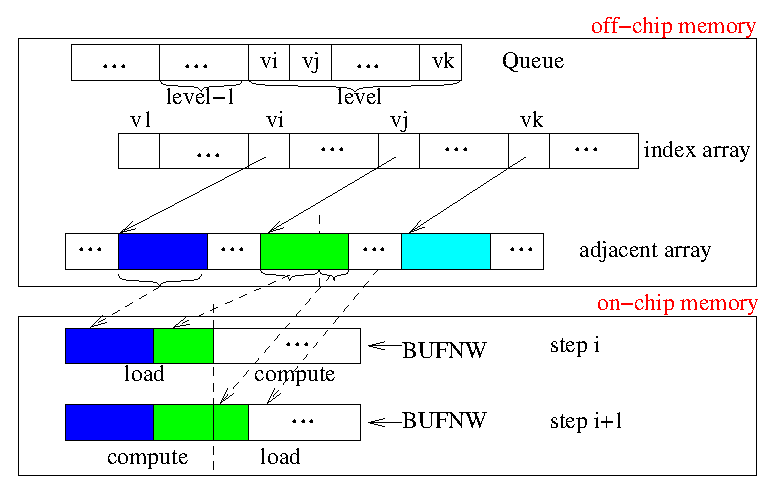
\includegraphics[width=5in,height=2.5in]{Img/Chap_Algorithm/db}
		\caption{double-buffering中的片外和片内存储映像。}
		\label{fig:db}
	\end{center}
\end{figure}


\subsection{数据流体系结构中硬件锁同步的优化}
当线程遍历同一级中顶点的邻接点时,如果存在相同的邻接点,冲突发生,这时需要某种同步方式处理冲突情况。粗粒度锁同步对整个邻接数组分配一个全局锁,
每个线程需要获取顶点遍历其邻接点都需要先获得锁。然而,事实上,并不是每次都存在冲突,所以这种粗粒度锁效率较低。细粒度锁给每个顶点赋予一个
锁变量,显然,在常规体系结构上,需要一个和邻接数组一样大小的数组保存锁变量。在本研究中的多核体系结构中,锁数组的大小通常超过片内存储而产
生大量的片外存储的访问,这导致性能显著下降。IBM Cyclops64处理器提供了硬件支持的细粒度锁同步机制-Synchronization State Buffer(SSB)\citep{ssb-isca07}。和
Cray MTA-2中的full/empty存储位机制不同,SSB在存储控制中增加了一个小的额外存储,记录和管理正在使用的锁同步的数据单元的状态。当某个存储地
址需要一个线程单独访问,SSB分配一个空间纪录该存储位置,而不是一开始就为可能使用的锁分配所有的空间。SSB的提出基于一个重要而合理的假设:在
任何时刻,被同步的存储位置只有很小的一部分正在被使用。也就是说,尽管在程序运行的整个生命周期,大量的锁同步需要使用,但在具
体的某个时刻,只有相当少部分的锁同步被使用。图\ref{fig:ssb-entry}是SSB中一个元素的结构。每个元素由4部分组成:1)地址域保存需要锁同步的存
储地址;2)参与同步的线程ID;3)8位的计数器;4)4位状态域支持16种不同同步操作状态。具体的SSB实现和解释请阅读参考文献。这里基于SSB实现了BFS中
的细粒度同步并行算法,算法\ref{algo:ssb}中的{\it swlock\_l} 和{\it sunlock}是对存储地址的获取锁和释放锁的函数。
\begin{figure}[!htbp]
	\begin{center}
		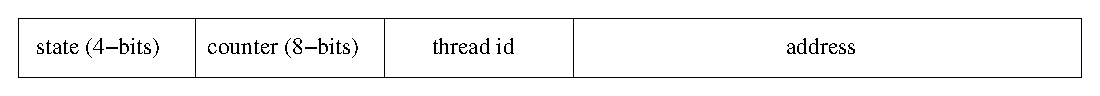
\includegraphics[scale=0.6]{Img/Chap_Algorithm/entry}
		\caption{SSB结构} \label{fig:ssb-entry}
	\end{center}
\end{figure}

\begin{algorithm}\label{algo:ssb}
	{\bf  BFS based on SSB on IBM Cyclops64}
	{\bf for} $w \in NW_{level}$ {\bf pardo}\\
	\hspace*{1pc}{\it rt = swlock\_l(\&(d[w]), \&dd);}\\
	\hspace*{1pc}{\bf if} rt == 0\\
	\hspace*{2pc}{\bf if} $d[w]<0$ {\bf then}\\
	\hspace*{3pc}enqueue $w\rightarrow Q_{level+1}$\\
	\hspace*{3pc}$d[w]\leftarrow d[v]+1$\\
	\hspace*{3pc}$\sigma[w]\leftarrow \sigma[w]+\sigma[v]$\\
	\hspace*{3pc}append $v\rightarrow P[w]$\\
	\hspace*{2pc}{\bf else if} $d[w]=d[v]+1$ {\bf then}\\
	\hspace*{3pc}$\sigma[w]\leftarrow \sigma[w]+\sigma[v]$\\
	\hspace*{3pc}append $v\rightarrow P[w]$\\
	\hspace*{2pc}{\it sunlock(\&(d[w]));}\\
	\hspace*{1pc}{\bf else if} $d[w]=d[v]+1$ {\bf then}\\
	\hspace*{2pc}{\bf while} ((rt = {\it swlock\_l(\&(d[w]), \&dd))} != 0);\\
	\hspace*{2pc}$\sigma[w]\leftarrow \sigma[w]+\sigma[v]$\\
	\hspace*{2pc}append $v\rightarrow P[w]$\\
	\hspace*{2pc}{\it sunlock(\&(d[w]));}
\end{algorithm}

评价图算法
性能的主要指标使用Bader等提出用于评价HPCS高性能计算机系统的基准测试程序SSCA2中的TEPS(traversed edges per
second)。假设顶点个数是$n=2^{scale}$,边数是$E(n)$\footnote{有时候为了简化问题规模,图遍历时只选择权值能被8整除的边},程序的运行时间用$T(n)$表示,TEPS定义
为平均每秒访问的边数$TEPS(n)=\frac{n*E(n)}{T(n)}$。实验测试了并行算法的弱可扩展性和强可扩展性。在传统的高性能计算机系统上,如果并行程序能够
获得高的弱可扩展性即可,即主要追求通过同时增加处理器和问题规模获得加速。在大规模多核体系结构中,处理核的数量正逐渐增加,但每个核的处理速度却呈
下降趋势,主要通过增加并行性来提高程序性能。因此,更合理的评价是在固定问题规模而只增加核的数目条件下测试并行程序的加速比。这意味者强可扩展性
应称为大规模多核上细粒度并行算法的更重要评价参数。事实上,这种要求也有利于在大多数情况下只能运行小规模程序的模拟器上开发和评价算法。
\begin{figure}[htbp]
	\begin{center}
		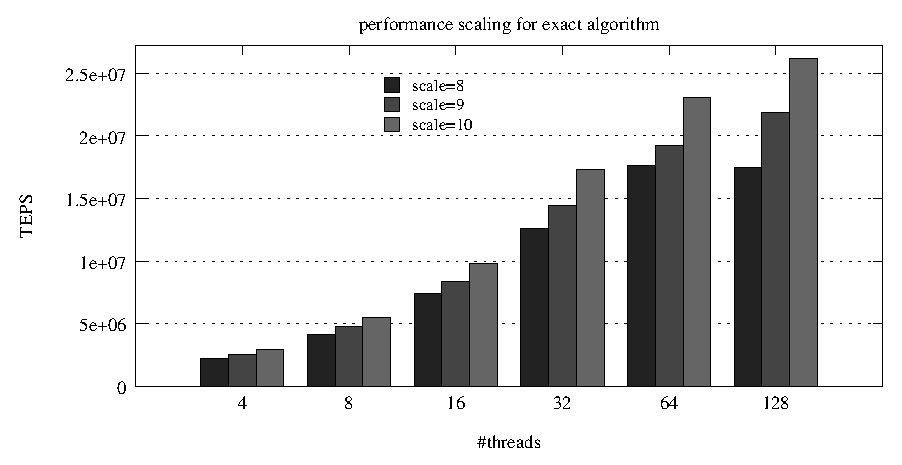
\includegraphics[scale=0.6]{Img/Chap_Algorithm/teps}
		\caption{并行介度中心算法的TEPS性能} \label{fig:teps}
	\end{center}
\end{figure}

图\ref{fig:teps}
是并行程序的TEPS性能。和SSCA2中的简单细粒度并行算法相比较,优化后的细粒度并行算法大大减低了运行时间而且
显示了随线程规模良好的可扩展性。尽管问题规模相当小,优化的细粒度并行算法仍然在线程数小于32时取得了线性加速比。在测试的最小问题规模为$scale=8$中,
当线程个数超过128时没有明显的性能提高,但在更大的问题规模$scale=9,10$时,算法也能取得加速比。注意到并行算法的中粒度和细粒度并行性的获得都和顶点
的度数有关。$scale=8$的情况下,图中的顶点的最大度只有64,因此存在的并行性导致在128个线程时不能获得好的性能; $scale = 9,
10$时,最大度分别是94和348,算法依然能够获得一定的扩展性能。


\section{科学计算-高性能稠密矩阵算法}\label{sec:PM_mm}
本节基于一种流行的细粒度多线程众核结构GPU上验证渗透算法设计模型的对稠密矩阵乘算法优化的有效性。首先介绍稠密矩阵乘算法基本概念和在众核上性能优化存在的问题。然后,描述在CUDA体系结构和编程模型中,基于渗透模型的稠密矩阵乘的流水线算法设计。进一步,基于NVIDIA GPU的体系结构(Fermi)提出一种更好隐藏长延迟指令的优化流水线的指令调度算法。

\subsection{稠密矩阵乘算法介绍}
稠密矩阵运算是科学计算和工程计算中的重要问题,是基础线性代数子程序(BLAS)库重要的一个核心算法。该规范定义DGEMM为 C := alpha * A * B + beta * C,其中A,B和C分别是m * k, k * n, m * n的矩阵。DGEMM的一个简单实现是三层循环嵌套。由于分块矩阵-矩阵乘法实现了更多的数据复用和更高的有效内存帶宽,分块矩阵乘法算法在具有内存层次结构的处理器上会有更高的性能。

大量的研究工作指出,全局内存的延迟和帶宽对DGEMM的效率有重要影响。对GPU上的分块DGEMM算法,A,B,C三个矩阵分别被分成bm*bk,bk*bn,bm*bn大小的块,这些块分别分布成M*K,K*N,M*N的网格,其中M=m/bm, N=n/bn, K=k/bk。计算是在一个二维的线程块网格上完成的,每一C的子块分配给一个线程块。也就是说,共有M*N个线程块,每个线程块都需要分别获取K个A和B的子块。这些内存读从全局内存读取了M*N*K*bm*bk+M*N*K*bk*bn=m*n*k*(1/bm+1/bn)个双精度浮点数。分块算法让全局内存帶宽需求减少了2/(1/bm + 1/bn)倍。此外,由于A和B的块都是首先加载到共享内存中,数据将被重用多次,从而减少了全局内存访问的代价。

GPU上的内存层次结构抽象为三个层次:片外内存(全局内存),片上内存(cache或者共享内存)和寄存器文件。从全局内存层次到寄存器层次,相邻层之间的帶宽增加且延迟减少。因此,分块算法通常包含两层分块。对于我们分块DGEMM算法而言,我们将从全局内存到共享内存层次的分块称为共享内存分块。由于共享内存和寄存器文件之间存在带宽和延迟的差距,共享内存中的子矩阵的分块对于重用寄存器中的数据是必要的。我们将这一层分块称为寄存器分块。此外,为了最大限度地提高浮点执行单元的效率,共享内存和寄存器文件的利用是另一个关键因素。举例来说,共享内存中的数据布局和访问模式应该仔细安排以避免bank冲突,这些冲突会导致额外的访存延迟。每个线程使用的寄存器数量也应该平衡以保持足够的线程并发来掩盖延迟。

算法\ref{algo:dgemmV0}是具有全局内存和共享内存层次的两层分块算法。矩阵A在进行矩阵乘之前转置了。本文中的实验结果包含了转置的开销,占了大约1\%的算法执行时间。在伪代码中还有几个未定义的参数(如bm,bn…),这些参数对性能有直接影响。
\begin{figure}[htbp]
	\begin{center}
		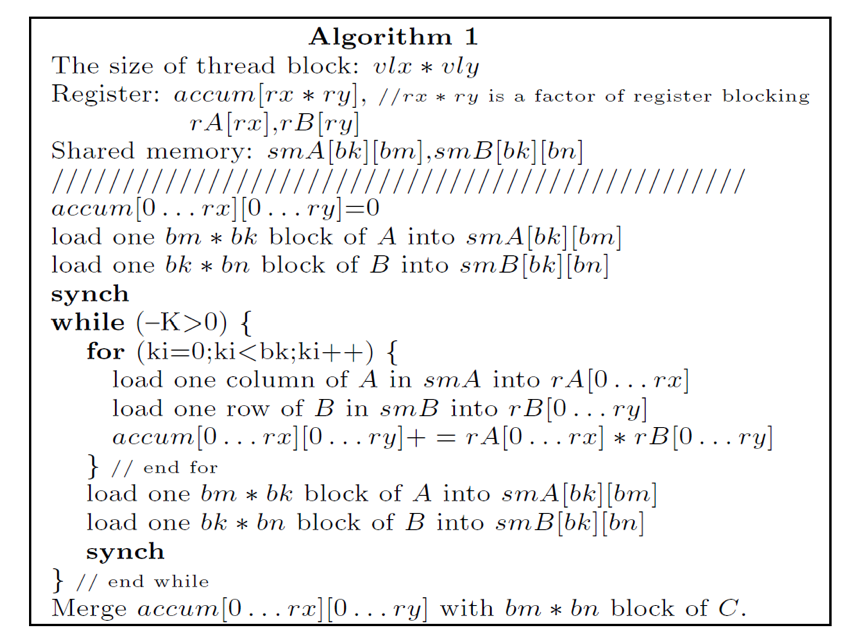
\includegraphics[scale=0.8]{Img/Chap_Algorithm/dgemmV0}
		\caption{DGEMM例程基础算法} \label{fig:dgemmV0}
	\end{center}
\end{figure}

\subsection{渗透模型的流水算法设计}
对算法模型的深度分析表明采用更宽的如128位内存操作可提高获得更高的浮点性能的空间\citep{},但需要新的线程-数据映射策略。两个warp加载长度为64(bm或bn)的A/B的一列/一行,每个线程加载一个64位的双精度数据。如果使用128位的内存指令,我们只需要32个线程(1个warp),每个线程加载两个双精度数据(128位)。因此我们将线程块由64*4改为32*8。图7描述了两种不同内存指令模式下数据-线程的映射情况。其中左边的图展示了使用64位内存取数指令将64*16的数据块从全局内存读取到共享内存中的过程,右边的图展示了使用128位内存取数指令的情况。

\begin{figure}[htbp]
	\begin{center}
		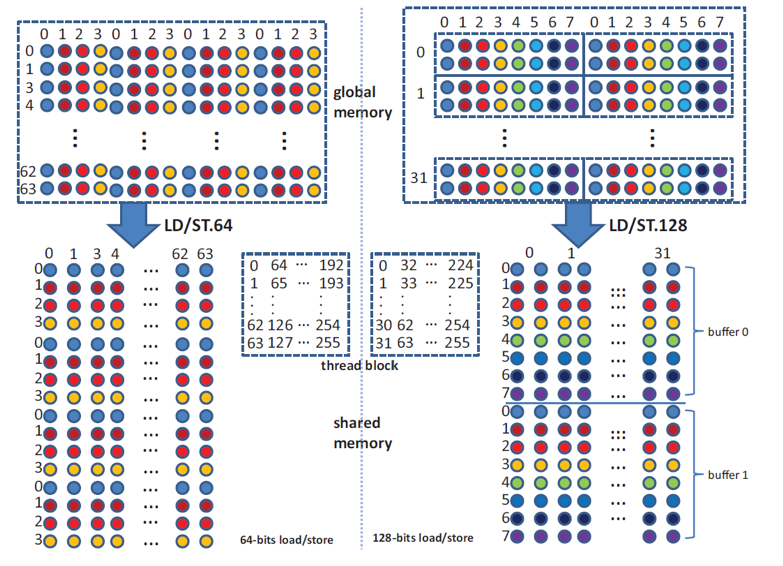
\includegraphics[scale=0.8]{Img/Chap_Algorithm/DGEMMpipeline}
		\caption{全局内存和共享内存间数据传输的数据线程映射。这张图由虚线分为两部分。左边阐明了算法2使用64位内存指令的映射。右边阐明了算法3使用128位内存指令的映射。} \label{fig:DGEMMpipeline}
	\end{center}
\end{figure}

假设矩阵以列向布局存储在全局内存中,而块以行向布局存储在共享内存中。如图~\ref{fig:DGEMMpipeline}所示,对大小为64*16的的块,使用64位内存指令时每个线程需要发射4条存取指令,而128位模式下每个线程只需要发射2条存取指令。例如,发射4条64位内存指令时,线程0…63取0,4,8,12列(图中蓝色的列),线程64…127取1,5,9,13列(图中黑红色的列),线程128…191取列2,6,10,14列(图中红色的列),线程192…255取3,7,11,15列(图中黄色的列)。在共享内存中,64个双精度数(64位)的一列存储为一行,然后由一列64个线程连续访问。图~\ref{fig:DGEMMpipeline}中右图阐明了128位内存操作模式下相应的数据-线程映射。线程0…31取0,8列(图中蓝色的列),线程32…63取1,9列(图中黑红色的列)。类似地,每一列线程通过2条128位内存指令取2列(同样颜色的列)

如果我们把Fermi的存储层次抽象为由全局内存和共享内存组成的两层,Fermi与其它带有显示的软件控制内存架构的众核架构如IBM Cell和IBM Cyclops64处理器非常类似。经验表明,在低延迟的内存中使用双缓冲的软件流水是一种有效的把计算和跨内存层次的通信重叠的方法。
为了实现一个双缓冲策略,我们将大小为64*16的块分为两块64*8大小的块。当前半部分用于计算矩阵C时,取后半部分数据的指令也会发射。线程调度程序负责将计算与内存操作重叠。双缓冲算法如图8所示。在伪代码中,我们将smA/B[0…bk/2-1][bm]映射为图7中的缓冲区0,smA/B[bk/2-1…bk-1][bm]映射为缓冲区1。在while循环中,指令被同步操作分组为内存和计算指令。由于它们操作不同的共享内存缓冲区,内存操作与计算可以并行进行。这些指令间没有数据依赖,因此还有空间通过指令调度优化来隐藏内存延迟。

新算法没有使用额外的寄存器实现双缓冲策略。事实上,一个重要的变化是使用了高延迟的128位内存指令。此外,为了确保下一块数据在计算之前完全被加载到共享内存中,双缓冲策略迫使我们在while循环中使用另一条同步指令。显然,除了128位内存指令的高延迟,额外的同步也带带来额外的延迟。由于双缓冲算法的主要代价是额外延迟,因此我们认为这里有通过指令调度来隐藏这些延迟的空间。
\begin{figure}[htbp]
	\begin{center}
		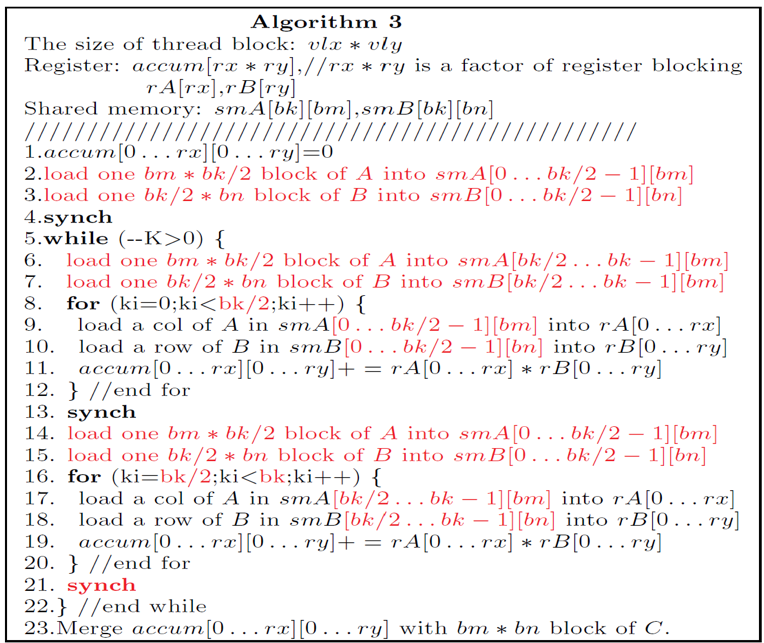
\includegraphics[scale=0.8]{Img/Chap_Algorithm/DGEMMPipeAlgo}
		\caption{双缓冲策略优化后的算法。} \label{fig:DGEMMPipeAlgo}
	\end{center}
\end{figure}


\subsection{体系结构相关的优化实现}
算法3中的while循环占用了大部分执行时间。我们的指令调度主要关注这段代码。在详细介绍指令调度的算法之前,我们首先计算出执行这段代码的指令组合比例。表3总结了指令组合的比例。如前所述,每个线程从全局内存加载一个元素(4字,在下文中,我们用一个元素指代128位的数据)到共享内存中两个缓冲中的一个(参看算法3中的6-7,14-15行)。由于没有内存到内存的指令,一次数据移动操作被转换为两条内存指令:一条加载指令(ld.gm.128)将数据从全局内存加载到寄存器,一条存储指令(st.sm.128)将数据从寄存器存储到共享内存中。每个while循环将发射4条指令来填充双缓冲区。现在让我们检查每个半缓冲区的两个内部循环。在每个ki循环中,每个线程将A的两个元素和B的两个元素读入寄存器,然后计算C的一个4*4的字块。内存操作有4条共享内存的加载指令(ld.sm.128)组成,计算操作由16条浮点指令(dfma)组成。对bk=16来说,总共有64条ld.sm.128和256条dfma指令。此外,我们需要10条整数指令和一条分支指令来进行地址计算和循环控制。

为了方便调度指令执行顺序,我们测量了while循环中使用的指令的流水线延迟。表3列出了指令延迟。由于数据依赖性,我们将延迟分为两种类型:写后读(RAW)和读后写(WAR)。例如,假设指令y依赖于指令x,写后读延迟就是从指令x发射到读取指令x写入寄存器的值的y指令可以发射这中间经历的时钟周期数。读后写延迟是从指令x发射到写入指令x读取寄存器的y指令可以发射这中间经历的时钟周期数。

\begin{figure}[htbp]
	\begin{center}
		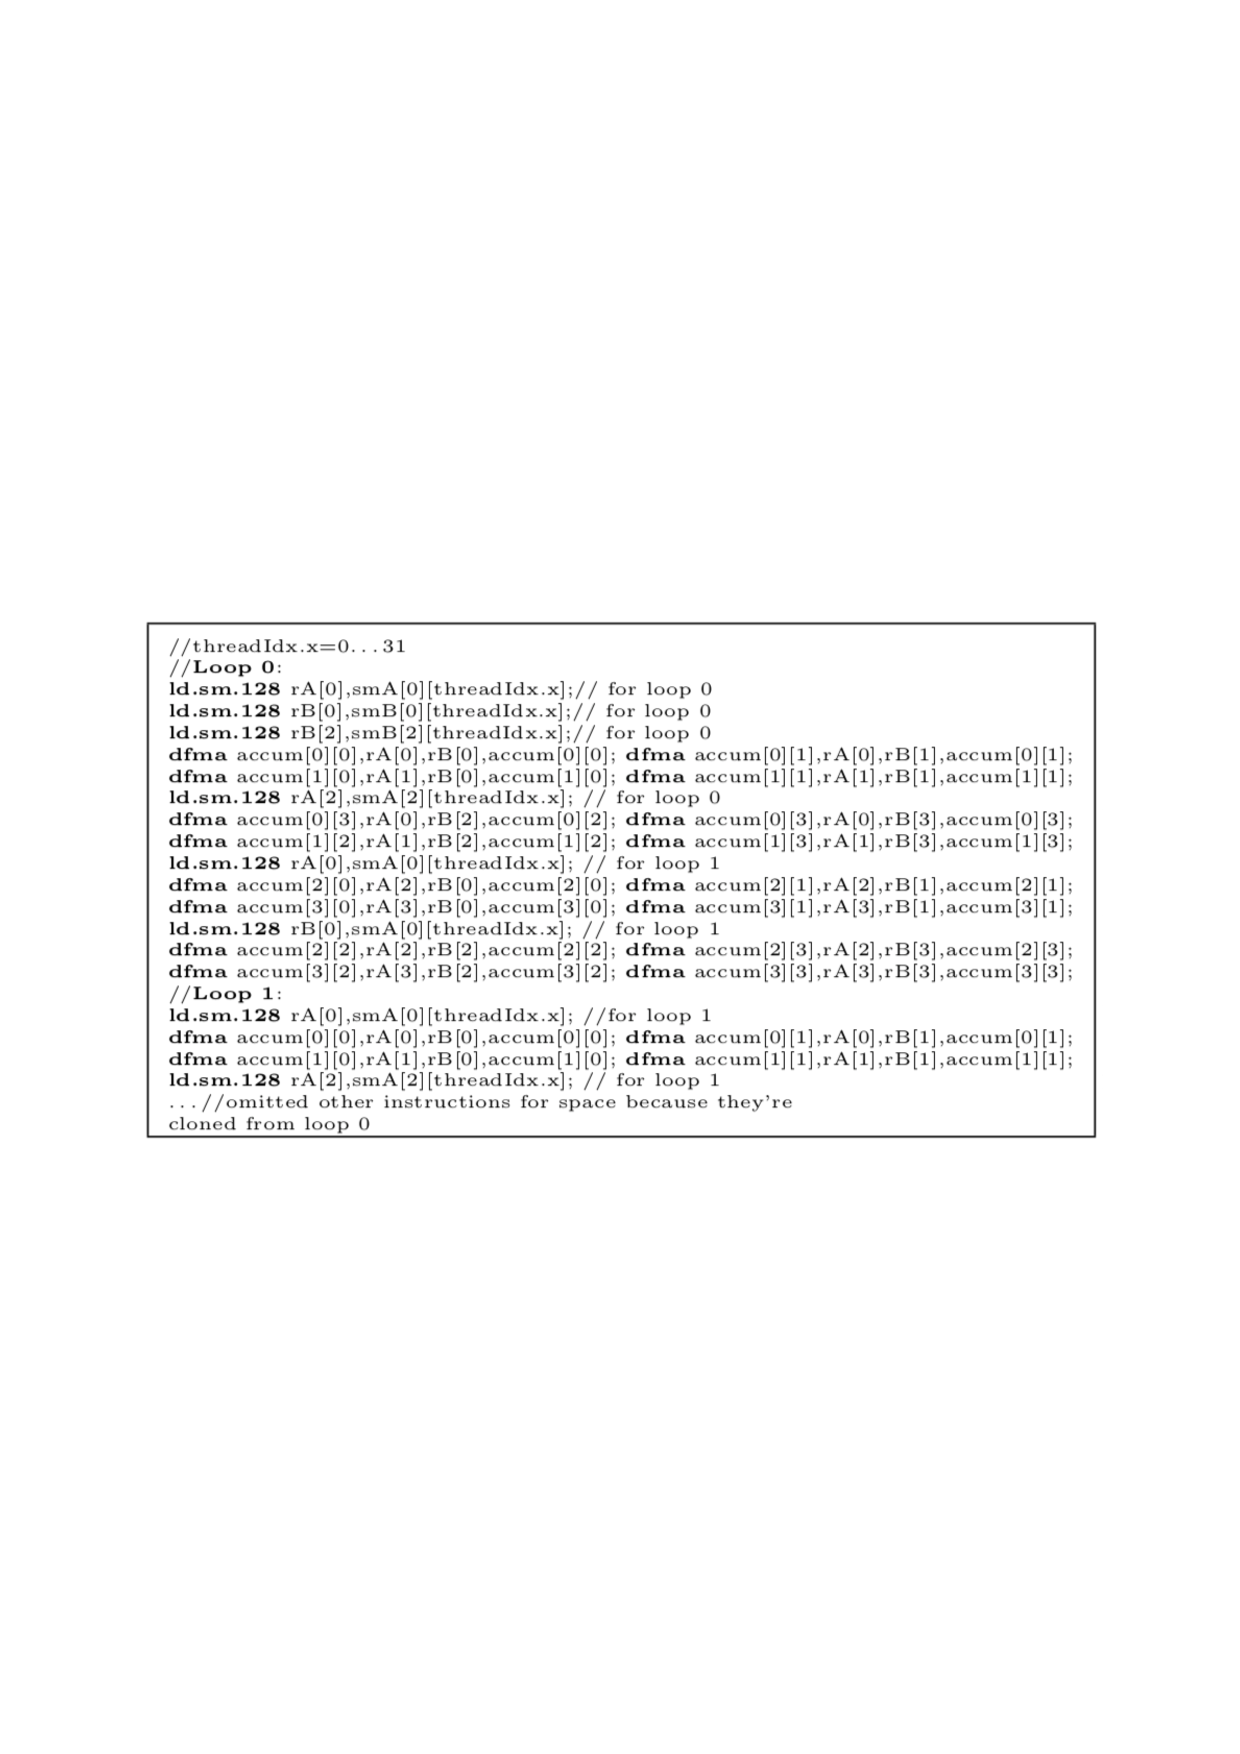
\includegraphics[scale=0.8]{Img/Chap_Algorithm/InstrSched}
		\caption{内存循环指令调度算法。} \label{fig:InstrSched}
	\end{center}
\end{figure}

指令流的执行是根据测量到的延迟来调度的。给定一个指令序列,我们扫描代码,对于每条指令,我们计算该指令使寄存器的值可用需要多长时间。例如ld.gm.128 r2,[r1]指令,寄存器r2,r3,r4,r5的值在指令发出几百个循环后才可用。在我们的调度算法中,我们将这种延迟称为寄存器的有效时间(即r2的有效时间为332∼1000个周期,这取决于数据是否缓存)。我们动态地构造了两个map表last\_raw和last\_war来记录每条指令的寄存器名及其有效时间(如last\_raw[r2] = 1000)。与此同时,我们跟踪直到当前指令发射的累计执行时间(tcurr)。我们会检测当前指令需要的寄存器是否处于last\_raw或last\_war表中。如果这些寄存器不在这两张表中,则由于没有数据依赖它的发射阻塞时间为0。否则,如果其中一个寄存器出现在两张表中的任意一张,则当前指令发射的阻塞时间由寄存器的有效时间和当前时间只差计算得到。例如,如果在指令 ld.gm.128 r2,[r1]扫描之后指令 st.sm [smA],r2,则它的发射阻塞时间为last\_raw[r2] - tcurr。假设ld.gm指令和st.sm指令之间有4条独立指令,这四条独立指令每条都有6个时钟周期的无阻塞发射到发射延迟,则观察到的ld.gm到st.sm之间的延迟(或者说st.sm额外阻塞的时间)是1000-(t\_curr=4*6+6)=970个时钟周期(st.sm有6个时钟周期的延迟)。指令调度的目标是使所有指令的累计延迟时间最小。


首先,我们重新排列每个内部for循环的指令序列。图~\ref{fig:InstrSched}展示了内部for循环中的前两个循环的指令重新排序示例。每个循环有4条ld.sm.128指令后面跟着16条 dfma指令。表面上看执行顺序不能改变因为寄存器rA[0…3]与寄存器rB[0…3]之间存在数据依赖。然后,如图~\ref{fig:InstrSched}所示,寄存器rA[0],rA[1]在前8条dfma指令执行后就释放了,寄存器rB[0], rB[1]在前12条dfma指令执行完之后就被释放了。这一观察结果表明,在展开的循环中插入这些加载指令以最小化阻塞时间是可行的,因为最多只用搜索8个可能得插入点。然后,我们添加了4条load/store指令的调度,这些指令将数据从全局内存加载到共享内存。由于这些指令与其它受同步限制的160条指令之间没有数据依赖关系,因此我们可以为这四条指令在这160条指令之间穷举搜索最好的插入点。最后,在两条st.sm.128指令中的第二条被调度后,我们我们从这条指令的插入点之后搜索同步指令的插入点。


\begin{figure}[htbp]
	\begin{center}
		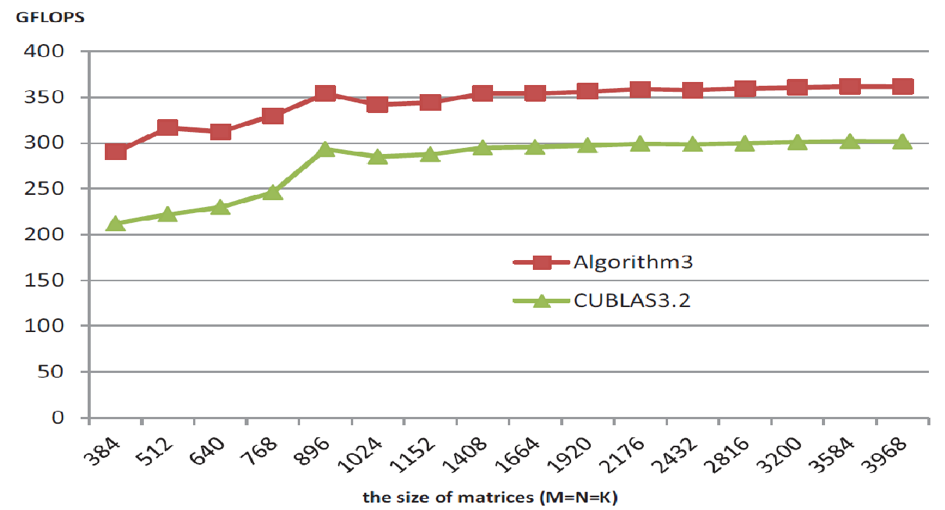
\includegraphics[scale=0.8]{Img/Chap_Algorithm/DGEMMPerf}
		\caption{优化的DGEMM与NVIDIA CUBLAS的性能比较。} \label{fig:DGEMMPerf}
	\end{center}
\end{figure}

图~\ref{fig:DGEMMPerf}报告了它们的总体性能改进。它描绘了我们最终版本DGEMM函数的性能。与CUDA3.2相比,它提高了20\%的浮点性能,并达到峰值362gflops /s(浮点效率为70\%)。虽然我们的优化策略的组合确实提高了性能,但是成功的一个主要前提是我们必须手工用汇编代码来实现优化的程序。事实上,我们之前的分析表明,在选择最优的分块算法之后,DGEMM程序的性能瓶颈是延迟。特别地,128位内存指令的使用让这个问题变得更糟糕。然而,我们的优化策略减轻了指令延迟的影响,提高了性能。

\section{相关工作}

\section{总结与评述}

\section{文献索引和笔记}

\end{flushleft} %%第四章
%%\input{Tex/Chap_System.tex}
\chapter{应用实例}\label{chap:application}

\begin{flushleft}  %% 左对其(临时添加)
\setlength{\parindent}{2em} %% 首行缩进(临时添加)

\qquad  

\section{导言和背景}
\subsection{Introduction (导言)}
\subsection{Background (背景)}

\makeatletter
\newenvironment{breakablealgorithm}
  {% \begin{breakablealgorithm}
  \begin{flushleft}
    \refstepcounter{algorithm}% New algorithm
    \hrule height.8pt depth0pt \kern2pt% \@fs@pre for \@fs@ruled
    \renewcommand{\caption}[2][\relax]{% Make a new \caption
      {\raggedright\textbf{\ALG@name~\thealgorithm} ##2\par}%
      \ifx\relax##1\relax % #1 is \relax
        \addcontentsline{loa}{algorithm}{\protect\numberline{\thealgorithm}##2}%
      \else % #1 is not \relax
        \addcontentsline{loa}{algorithm}{\protect\numberline{\thealgorithm}##1}%
      \fi
      \kern2pt\hrule\kern2pt
    }
  }{% \end{breakablealgorithm}
    \kern2pt\hrule\relax% \@fs@post for \@fs@ruled
  \end{flushleft}
  }
\makeatother

\section{COStream数据流编程语言及其在深度学习中的应用(于俊清)}
\subsection{引言}
近些年,多/众核架构已经被普遍认为是开发并行性的有效平台,一方面它为各类应用提供了强大的并行计算能力,特别是在数字媒体处理和科学计算等计算密集型的应用领域;另一方面它也将如何充分挖掘程序的并行性以及如何充分利用资源等问题暴露给了编程人员。传统的编程模型,如C、C++和Fortran,主要对应的都是单指令流和集中存储管理模式,无法很好的适合这种特殊的并行体系结构。当前比较流行的编程模型,如OpenMP和MPI,要求程序员必须熟悉并行系统的底层结构,编程人员设计并行程序时需要根据系统底层结构进行精心的任务划分、数据通信以及同步设计。导致程序性能受制于编程人员并行算法的设计和对并行系统的理解,增加了编程人员,尤其是各个应用领域编程人员的编程复杂度。
针对上述问题,数据流编程模型作为新的高效的并行编程模型被重新重视,编译器可以根据多核处理器体系结构的特点有效地将任务进行划分并映射到各个处理核上,生成适合于当前体系结构的可执行程序,大幅简化编程难度,提高程序执行的效率。

基于多核与分布式系统结构以及数据流编程模型的特点,华中科技大学的智能媒体计算与网络安全实验室设计并实现了一种面向数据流编程的编程语言与编译系统 -- COStream。语言的名称由3个关键字:Composite、Operator和Stream组合而来。COStream程序采用有向图来描述应用的处理过程,图中节点表示计算,边表示数据依赖,边的方向表示数据流动方向。



\subsection{COStream 数据流编程语言}
COStream是在C语言文法基础上加入了表征数据流图结构文法而形成的数据流编程语言,它实现了对数据流图最基本的抽象,方便数据流程序的编写。

\subsubsection{与 C 语言的关系}
(1)COStream 保留了 C 语言的全局变量声明, 在文件头部声明了全局变量名后, 可以在后续的函数,Composite 和 Operator 中使用。下面给出了一些示例代码:
\begin{algorithm}\label{algo:standard}
int i = 0; double j = 0.0; //支持整数和浮点数\\
int i = 1, j = 2, k = 3; //支持一条语句中声明多个变量\\
int i = 1e10, j = 0x16; //初始值支持科学记数法和16进制\\
int a[3] = { 1,2,3 };   //支持数组声明和赋初值
\end{algorithm}

(2)COStream 支持全局函数声明,但由于其是数据流编程语言,而非面向对象编程语言,不能通过 this 关键字来访问执行上下文, 因此全局函数多用来做一些数据计算的复用,下面给出一些示例:

\begin{algorithm}\label{algo:standard}
int sum(int a, int b)\{\\
\hspace*{1 pc} return a+b; // 最基础的加法运算\\
\}\\
double expr(double base, double x)\{\\
\hspace*{1 pc} return base**x; // 支持使用两个星号**来表示 base 的 x 次方\\
\}
\end{algorithm}
(3)COStream 支持的基础运算类型有: 
\begin{itemize}
    \item 双目运算符: + 加, - 减, * 乘, / 除, \% 取余, ** 乘方
    \item 位运算符: \& 按位与, | 按位或, \^{} 异或, << 左移, >> 右移
    \item 逻辑运算符: < > <= >= == != \&\& || !
    \item 单目运算符: + 正号, - 负号, ++ 自增, -- 自减
    \item 三目运算符: ? :
    \item 成员运算符: . 例如 S.a
\end{itemize}

但与 C 语言不同的是, COStream 抛弃了 C 语言中函数必须先声明后调用的限制, 而参考其它语言的文法, 规定函数的调用可以放在声明前, 实现方式为通过编译器在文法解析时的预处理, 优先将全局变量和函数声明信息存入符号表, 使得解析函数调用时可以直接从符号表中提取相关信息, 而非依赖上下文环境。

\subsubsection{Stream}
数据流(stream)是由一系列数据流成员(token)组成的序列,作为通信载体连接数据流图中各个计算单元(actor),它是对数据流图中通信边的抽象,为计算单元提供可并行操作的数据对象。组成stream的token是一种复合数据类型,运算主要是对token进行的。存储器中对数据流的安排对于程序员而言是透明的。COSteam代表token的stream声明类似于C语言的结构体,可以包括任意基本C数据类型(如int、float和double等)、字符串类型(string)和基本类型的数组等。数据流分为输入数据流和输出数据流两种类型。在SDF图中输入数据流对应actor的输入边,对actor是只读的;输出数据流对应actor的输出边,对actor是可读写的。一般来说,一个stream是一个actor的输入数据流同时又是另一个actor的输出数据流。

\subsubsection{Operator}

同步数据流图中最基本的组成单元和计算单元actor在COStream中由operator文法结构表示,operator在SDF中被抽象成一个结点,专门用来处理stream中的数据。operator定义了actor输入流、输出流和具体的处理过程。operator由头部定义和体定义组成,其中operator头部定义了该operator处理的输入、输出流以及operator名称,COStream暂时不支持匿名operator的定义。COStream中一个operator可以有多个输入流和多个输出流。Operator体包括declare(静态变量声明)、init(静态变量初始化)、work和window四个部分。其中,work函数是operator内最细粒度的运算,是operator的核心结构,是数据流程序迭代执行过程中每次执行计算的单元。对operator输入和输出缓冲区的访问操作也是在work中进行的。operator内部变量的声明部分(declare)主要是为了定义该operator的work在执行时是需要的一些静态变量,类似于C语言中static关键字修饰的变量,对于无状态的operator来说,这部分可以为空。init定义了operator开始执行时需要进行的初始化工作。window规定输入、输出数据流缓冲区的窗口类型并决定operator对输入、输出流中数据访问的窗口大小。下面给出一个示例, 该示例描述了一个产生1,2,3,4,5,6...的自然数序列的数据流。

\begin{algorithm}\caption{产生自然数序列的数据流示例}\label{algo:operator-example}
  stream<int x>S;\\
  S = Source()\{\\
  \hspace*{1 pc} int i;\\
  \hspace*{1 pc} init \{i = 1;\}\\
  \hspace*{1 pc} work \{\\
  \hspace*{2 pc} S[0].x = i;\\
  \hspace*{2 pc} i++;\\
  \hspace*{1 pc} \}\\
  \hspace*{1 pc} window\{\\
  \hspace*{2 pc} S tumbling(1);\\
  \hspace*{1 pc} \}\\
  \};
\end{algorithm}

该示例的第1行描述了一个由整数int组成的数据流 S, 可以使用S[0]来访问数据流 S 的窗口中第一个位置, 而 S[0].x 表示该位置的成员 x (其类型为 int)。 接着,在示例的3~4行,Operator Source 声明了一个静态变量 i 并赋初值为1,接下来的执行流程为:执行一次 work 内部的语句->翻转窗口window->执行一次work内部语句->翻转窗口 window->…->执行一次work内部语句->翻转窗口window, 可以看出, 每次执行 work 都会使得窗口第一个位置的 x 赋值为自然数序列变量 i 的最新值 同时 i 自增,然后通过 window 中的窗口翻转将该数据传给后续的 Operator。

下面详细讨论COStream中的窗口机制。
\begin{figure}[htbp]
	\centering
	% Requires \usepackage{graphicx}
	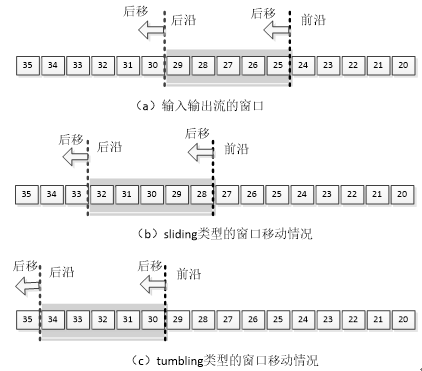
\includegraphics[width=5in]{Img/Chap_Application/Yu/operator.png}\\
	\caption{operator的窗口机制}\label{fig:operator}
\end{figure}
COStream对流中的数据访问采用窗口机制,窗口用前沿和后沿界定,前沿和后沿的距离就是当前operator执行时可操作的输入、输出缓冲区的大小,它由window中的参数确定。COStream中窗口类型有两种:sliding和tumbling。sliding代表滑动窗口类型,这种窗口有peek,pop和push操作,一般用于输入流;而tumbling则代表翻转窗口类型,只有push和pop操作,该种类型窗口既可以用于输出流也可以用于输入流。对于输入流主要的操作有pop和peek。pop操作删除输入流中最先到的token,并返回该token。peek(i)返回输入流中距离输入流窗口前沿的第i个token。对于输出流主要操作是push,push操作是将计算得到的token输出到输出流,对缓冲区的使用是从前沿到后沿的。operator一次执行完成后同时移动窗口的前沿和后沿。图\ref{fig:operator}(a)图描述COStream中的输入输出流的窗口示意图,图\ref{fig:operator}(b)和(c)分别表示如果(a)对应的窗口分别是sliding(5,3)和tumbling(5)时,一次operator执行完成后窗口的移动情况。


\subsubsection{Composite}
在面向过程编程的 C 语言中, 程序入口为 main 函数, 在函数中使用多种控制语句来编写程序。与之不同,在面向数据流编程的 COStream 语言,程序入口为 Composite Main,在其内部通过将不同 Operator 用Stream 变量进行连接来构造数据流图。

COStream定义的用于连接不同节点构造数据流图的Composite结构属于高层次(相对于operator)的复合结构,代表一个由一个或若干个operator组成的可重用的数据流图结构,它是对SDF图中可复用的子图的抽象。它既可以完整的表示一个数据流程序的数据流图结构,也可以作为子数据流图结构被调用。下面是一个略去细节信息的抽象 composite 例子,它表示输入的数据流 S 依次经过了3个 operator 的处理后,计算得到了输出流T。

\begin{algorithm}\label{algo:operator}
Composite Main(input S, output T)\{\\
 \hspace*{1 pc} S0 = first(S);\\
 \hspace*{1 pc} S1 = second(S0);\\
 \hspace*{1 pc} T  = third(S1);\\
\}
\end{algorithm}

composite主要由composite头部和composite体组成。composite头部表明该composite的输入输出边参数、composite参数以及composite的名称,COStream不支持匿名composite。composite的输入输出边参数是用来确定在生成SDF图时该composite结构所形成的子图与SDF图中其他节点的连接关系。composite参数主要是指composite结构在实际被调用时需要从调用处传入的参数,可以根据参数的情况决定composite最终子图的结构,另外该参数也可以在composite内部被使用。composite体主要有如下2部分组成:一部分是composite内部需要使用的变量的定义和一些相关的操作语句;另一部分是composite内部的子图结构,它由一个或若干operator组成,每个operator根据输入流、输出流的依赖关系连接成图,是composite的核心结构。Composite结构在编译阶段被扩展,经过编译数据流程序的数据流图子结构将被扩展成完整的数据流图。

\subsubsection{多输入多输出流的连接方式}

composite可以同时有多个输入多个输出边。下面的数据流程序例子反映了上述语言特点。

\begin{algorithm}\label{algo:operator}
composite M (output K,L,input G,H) \{		//1\\
 \hspace*{1 pc} stream<int x> I=O(G)\{\}			//2\\
 \hspace*{1 pc} stream<int x> J=P(H)\{\}			//3\\
 \hspace*{1 pc} stream<int x> K=Q(I;J)\{\}			//4\\
 \hspace*{1 pc} stream<int x>L=R(J)\{\}			//5\\
\}									//6\\
composite Main\{						//7\\
 \hspace*{1 pc} …\\
 \hspace*{1 pc} (stream<int x>C,stream<int x> D) = M(A,B)\{\}	//8\\
 \hspace*{1 pc} (stream<int x>E,stream<int x> F) = M(A,B)\{\}	//9\\
 \hspace*{1 pc} …\\
\}
\end{algorithm}

\begin{figure}[htbp]
	\centering
	% Requires \usepackage{graphicx}
	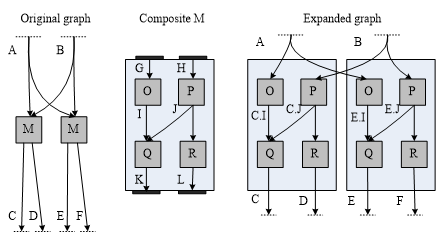
\includegraphics[width=1.0\textwidth]{Img/Chap_Application/Yu/multi.png}\\
	\caption{多输入多输出流连接方式}\label{fig:multi}
\end{figure}

图\ref{fig:multi}描述了行1至行9的程序片段所反映的数据流图调用、扩展过程:由Original graph扩展为Expanded graph。Original graph包含了2个composite结构M,第一个M将输入流A和B计算后得到输出流C和D,第二个M将输入流A和B计算后得到输出流E和F。行1定义了M的输入流为G和H,输出流为K和L。行8表示当M在Main中第一次被调用时,输入流和输出流发生实例化:G=A,H=B,K=G以及L=D。在Expand graph中M因为被调用2次而实例化成2份,所以M中的中间流I和J也被实例化为2份:C.I,C.J和E.I,E.J。这些子流图因被调用而实例化展开的过程在编译器编译时完成,经过编译后,数据流程序的流图结构将被扩展成完整的数据流图。

\subsubsection{pipeline 连接方式}

\begin{figure}[htbp]
	\centering
	% Requires \usepackage{graphicx}
	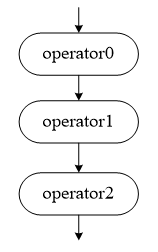
\includegraphics[width=0.25\textwidth]{Img/Chap_Application/Yu/pipeline.png}\\
	\caption{pipeline连接方式}\label{fig:pipeline}
\end{figure}

有时候我们会想要编写这样一种数据流结构: 每个 operator 的输入恰好是上一个 operator 的输出,即数据流在全局或局部保持单向传递,有时 operator 还可以复用。例如对应图\ref{fig:pipeline}中有3个 operator 的示例:

\begin{algorithm}\label{algo:costream}
Composite Main(input<int x> S0)\{\\
 \hspace*{1 pc} stream<int x>S1,S2,S3;\\
 \hspace*{1 pc} S1 = operator0(S0);\\
 \hspace*{1 pc} S2 = operator1(S1);\\
 \hspace*{1 pc} S3 = operator2(S2);\\
\}
\end{algorithm}

在这种情况下, 我们最关心的是输入流变量 S0和输出流变量 S3,而数据流变量S1,S2是多余的信息,实际上我们并不关心中间变量。在其它函数式编程语言中,我们可以使用 compose(组合)这个操作符来描述这种结构:

\begin{algorithm}\label{algo:costream}
operator3 = compose(operator0,operator1,operator2)\\
S3 = operator3(S0)
\end{algorithm}

等价于

\begin{algorithm}\label{algo:costream}
S3 = operator2(operator1(operator0(S0)))
\end{algorithm}

那么在COStream 数据流编程语言中, 有没有这种”串联”形式的组合结构呢?答案是有的, 这就是 pipeline 结构, 下面给出对应示例:

\begin{algorithm}\label{algo:costream}
Composite Main(input<int x> S0)\{\\
 \hspace*{1 pc} S3 = pipeline(S0)\{\\
 \hspace*{2 pc} add operator0();\\
 \hspace*{2 pc} add operator1();\\
 \hspace*{2 pc} add operator2();\\
 \hspace*{1 pc} \}\\
\}
\end{algorithm}

pipeline结构是由一串连续的composite调用组成,它们在pipeline结构中出现的先后顺序决定了它们在数据流图中的依赖关系。pipeline是单输入流单输出流,COStream规定能够在pipeline中被调用的composite也必须是单输入流单输出流。

\begin{algorithm}
  \caption{代码片段 A 和使用了 for/if 的代码片段 B 等价}
  \label{algo: pipeline}
  {\bf 代码片段 A}\\
  Composite Main(input<int x> S0)\{\\
    \hspace*{1 pc} S3 = pipeline(S0)\{\\
    \hspace*{2 pc} add operator0();\\
    \hspace*{2 pc} add operator1();\\
    \hspace*{2 pc} add operator0();\\
    \hspace*{2 pc} add operator1();\\
    \hspace*{2 pc} add operator0();\\
    \hspace*{2 pc} add operator1();\\
    \hspace*{1 pc} \}\\
  \}\\
  {\bf 代码片段 B}\\
  Composite Main(input<int x> S0)\{\\
    \hspace*{1 pc} S3 = pipeline(S0)\{\\
    \hspace*{2 pc} for(int i=0;i<3;i++)\{\\
    \hspace*{3 pc} if(i\%2==0)\{\\
    \hspace*{4 pc} add operator0();\\
    \hspace*{3 pc} \}\\
    \hspace*{3 pc} else\{\\
    \hspace*{4 pc} add operator1();\\
    \hspace*{3 pc} \}\\
    \hspace*{2 pc} \}\\
    \hspace*{1 pc} \}\\
  \}
\end{algorithm}

COStream引入add操作将operator和composite调用添加到pipeline中。 此外, pipeline 的结构体中支持使用 if 、for、while 语句等来控制 operator 的组合, 如算法\ref{algo: pipeline}所示,我们可以把代码片段 A 改写为代码片段 B,二者是等价的。





\subsubsection{splitjoin 连接方式}

\begin{figure}[htbp]
  \centering
  % Requires \usepackage{graphicx}
  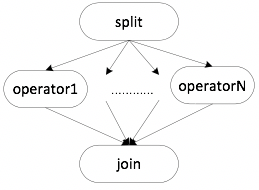
\includegraphics[width=0.5\textwidth]{Img/Chap_Application/Yu/splitjoin.png}\\
  \caption{splitjoin连接方式}\label{fig:splitjoin}
\end{figure}

除了 pipeline结构, 还有一种 splitjoin 结构用来描述数据流的分解与合并(图\ref{fig:splitjoin})。splitjoin结构由splitter、joiner以及一些composite调用组成,当一个流作为splitjoin结构的输入流时它被splitter分割,splitter根据splitjoin中composite调用情况产生一批满足相应条件的输出流作为不同的composite调用的输入流,这些composite调用的输出流作为joiner的输入流,joiner同样根据composite调用情况来合并各个输入流,将合并后产生的新的流作为joiner结点的输出,也是splitjoin结构的输出流。在splitjoin中splitter主要有两种方式:

\begin{itemize}	
  \begin{figure}[htbp]
    \centering
    % Requires \usepackage{graphicx}
    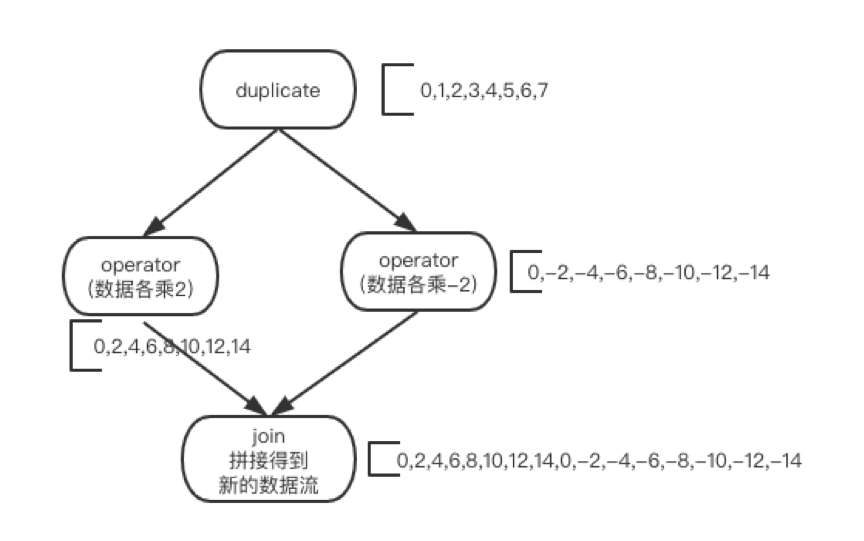
\includegraphics[width=0.8\textwidth]{Img/Chap_Application/Yu/duplicate.png}\\
    \caption{splitjoin-duplicate示意图}\label{fig:duplicate}
  \end{figure}

  \item {\bf duplicate方式}:该方式下所有的composite调用将会有完全相同的输入流(图\ref{fig:duplicate})。

  \begin{figure}[htbp]
    \centering
    % Requires \usepackage{graphicx}
    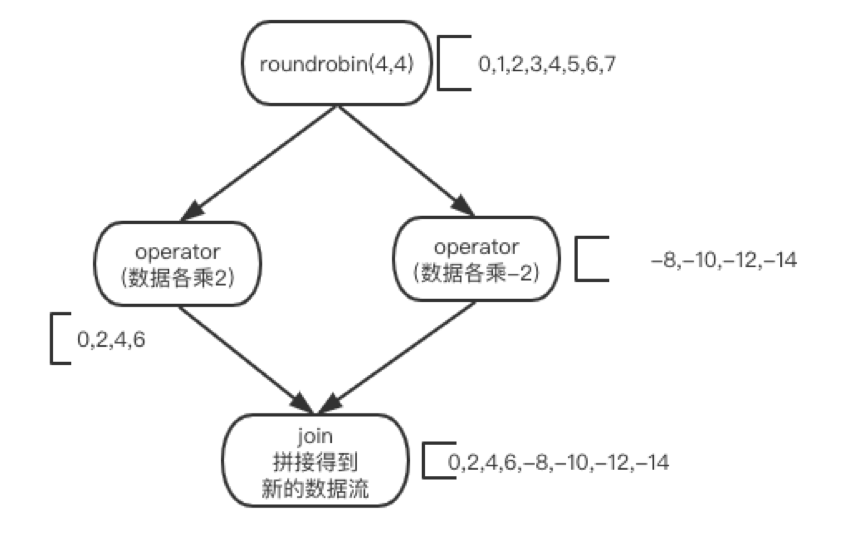
\includegraphics[width=0.8\textwidth]{Img/Chap_Application/Yu/roundrobin.png}\\
    \caption{splitjoin-roundrobin示意图}\label{fig:roundrobin}
  \end{figure}

  \item {\bf roundrobin(w1,…,wn)方式}:如图\ref{fig:roundrobin}所示,该方式下splitter将其输入流中的前w1个数据发送给第一个composite调用,接下来的w2个数据发送给第二个composite调用,以此类推,将最后的wn个数据发送给最后一个composite调用。对于joiner只有一种roundrobin方式。与pipeline结构类似,在splitjoin中调用的composite要求也是单输入流和单输出流的。
\end{itemize}

在COStream中splitter和joiner分别用关键字split和join表示,且可以和 pipeline 结构互相嵌套使用,下面是一个示例:

\begin{figure}[htbp]
  \centering
  % Requires \usepackage{graphicx}
  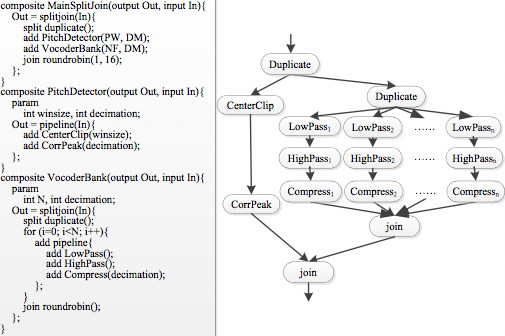
\includegraphics[width=1.0\textwidth]{Img/Chap_Application/Yu/vocodebank.png}\\
  \caption{vocodebank程序例子}\label{fig:vocodebank}
\end{figure}

图\ref{fig:vocodebank}的例子能够说明splitjoin和pipeline的层次性特点和使用特性。在图中左边部分是COStream的源码片段,右边是对应的数据流图。在本例中可以看到添加了层次性的结构有助于增加数据流程序编程的灵活性和可扩展性。另外,在splitjoin和pipeline中流能够被参数化,在本例composite VocodeBank中关于内置的pipeline调用次数可以有参数N来确定,通过N控制splitjoin结构的宽度,同样在pipeline中可以通过参数来控制pipeline的深度。

\subsubsection{内置 composite}

为了便于对文件操作,COStream对文件的I/O提供了内置composite支持,通过调用内置的文件I/O composite COStream可以完成对文件读写操作。FileReader和FileWriter是COStream为I/O提供的内置的composite接口。FileReader用于将文件中的数据读到流中,FileWriter是将流中的数据写到文件中。具体用法如下:

\begin{algorithm}\label{algo:costream}
stream<double x> A,B;			//1\\
A = FileReader(“data.bin”);		//2\\
FileWriter(B)(“result.txt”);
\end{algorithm}

行1表示将data.bin文件中的数据读入到数据流A中,行3表示将处理后输出的流B中的数据保存至文件result.txt。

此外,仍然存在许多常用功能性 Composite有待于内置在COStream编程语言中, 实验室的全体师生会积极进行版本迭代,进一步改进和优化COStream的编程语言结构设计。 

\subsection{COStream 编译器框架}

\begin{figure}[htbp]
  \centering
  % Requires \usepackage{graphicx}
  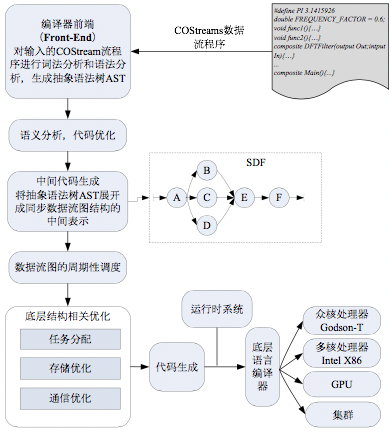
\includegraphics[width=0.8\textwidth]{Img/Chap_Application/Yu/compiler.png}\\
  \caption{COStream 编译器框架示意图}\label{fig:compiler}
\end{figure}

图\ref{fig:compiler}描述了COStream编译系统总体框架。COStream编译器的源语言为COStream数据流程序设计语言,目标语言根据目标结构不同生成不同底层语言,如C、C++(在x86平台上执行)和openCL(在 GPU 上执行)以及 Javascript(在跨平台的浏览器中执行)等,编译器通过调用底层语言编译器生成对应目标平台的可执行文件。下面详细介绍COStream编译系统的组成部分。

\begin{itemize}	
  \item {\bf 编译器前端}:编译器前端主要对COStream源程序进行分析,建立抽象语法树。对源程序的分析主要包括词法分析和语法性分析。在词法分析中,词法分析器从左到右地读构成源程序的字符流,把字符流分组为多个记号,记号是具有整体含义的字符序列。词法分析通常作为编译器的第一个阶段,产生记号序列,提交给语法分析使用。这里将词法分析作为语法分析的子程序来实现。当词法分析器收到语法分析器发出“取下一个记号”的命令时,词法分析器读入字符,识别出一个记号。COStream采用自底向上的语法分析过程。在语法分析中,将字符串或者记号划分为具有一定层次的多个嵌套组,每个嵌套组具有一个完整的含义。程序的层次性结构是通过递归规则来表达,在编译器中,语法分析器接受词法分析器提供的记号串,检查它们是否符合COStream的文法规则。如果文法匹配则通过规则建立语法树结点结构。源程序通过词语法分析最终将建立为一种由顶层语法树节点表示的层次性抽象语法树结构。COStream采用Lex和Yacc词语法生成器生成词语法分析器。

  \item {\bf 语义分析和代码优化}: 编译器对经过词语法分析形成的抽象语法树进行语义分析。语义分析是对COStream数据流程序进行类型检查以及为代码生成阶段收集类型信息。语义检查负责检验每个操作符的操作数是否满足源语言的说明。在该阶段除语义检查外还对源程序代码做机器无关优化。优化是在保持源程序语义的基础上减少代码占用空间,删除不必要的操作,降低程序运行时开销。为了提升程序的性能COStream实现了常见的机器无关优化,如常量传播和冗余代码删除等。该阶段得到最佳抽象语法树。
  \item {\bf 中间代码生成}: COStream编译器以同步数据流图作为中间表示,在该阶段分析编译器前端得到的抽象语法树,得到数据流程序中的composite调用关系和stream依赖关系,利用这两种关系将抽象语法树进行深层次的展开,得到一个只有operator通过stream相连的完整的数据流图的抽象语法树结构,利用此时的抽象语法树生成SDF图,该SDF图是编译器后续操作的基础。另外,在该阶段还需要对SDF图中的各个节点的工作量进行估计,确定SDF图中各个actor的负载情况。
  \item {\bf 数据流图的周期性调度}: 编译器根据中间表示的数据流图结构采用单出现调度策略 (Single Appearance Schedule,SAS) 得到静态平衡数据流图。编译器根据程序中各个operator的peek、pop和push值决定初态和稳态调度阶段的各个actor的执行次数,为后续的优化和代码生成提供依据。
  \item {\bf 底层结构相关优化}: 编译器根据不同底层系统结构特性,对COStream程序进行与底层结构相关的优化,主要从计算任务分配、存储优化和通信优化等方面对程序进行优化,在开发并行性的同时减小相应的开销,使数据流程序在执行时能够充分利用底层系统的资源,提高程序的执行效率。COStream主要针对X86、GPU和多核集群等目标系统做编译优化。在第\ref{section:x86}节中具体介绍面向X86共享多核架构下的相关优化。
  \item {\bf 代码生成}: 根据底层结构相关优化的结果和后端的体系结构以及目标代码的特性,设计最终目标代码的生成框架,生成高效的并行代码。
  \item {\bf 运行时系统}: 运行时系统是采用目标语言编写的静态链接库,包括支持目标代码运行所需要通信库和函数库,为代码生成提供辅助支持。
  \item {\bf 底层编译器}: 编译器将生成的目标底层代码交由底层语言编译器编译生成指定目标平台的可执行文件,完成整个编译过程。
  
\end{itemize}

\subsection{面向 X86 多核集群的 COStream 编译优化} \label{section:x86}

随着多核处理器平台日趋复杂,数据流程序的并行编译优化工作变得更加困难,其问题主要包括多处理器核的并行调度和对主存的访问延迟。针对数据流程序共享存储多核架构的结构特点,构造出高吞吐量低延迟的软件流水线调度,主要分为任务划分、阶段赋值、流水线执行三个步骤[12]。

\subsubsection{任务划分}

任务划分是在避免浪费处理器核的计算能力以及确保各处理器核间的任务负载均衡的基础上,使用合适的划分算法将数据流任务划分到合适的核上。任务划分的目的是根据数据流图(SDF图)中计算节点的负载和计算节点间的依赖关系构造高吞吐量低延迟的软件流水线调度,以最大化底层系统资源利用率。数据流程序要想充分利用系统资源就必须充分合理地利用其自身的数据并行性、任务并 行性和流水线并行性。在软件流水线调度中,流水线的启动间隔(Initiation Interval,II)是指相邻两次循环迭代进入流水线的时间间隔,II越小意味着吞吐率越大。任务划分的目的就是要最小化II。在软件流水中II是由流水线中各资源的处理时间决定,在X86中,资源主要是处理器核,那么影响程序最终执行性能的主要因素就是划分的负载均衡情况。

在进行任务划分前,需要对SDF进行预处理,包括扩大调度和融合相邻计算节点。扩大调度指的是以相同的扩大因子,成倍扩大每个计算单元稳态调度阶段的执行次数,这样可以减少同步开销对程序性能的影响。相邻计算节点的融合是指将两个独立且在数据流图中相邻的计算节点融合为一个计算单元。相邻计算单元融合操作保证了两个计算单元不会被分配到不同的处理器核上调度,这能够减少通信开销对程序的影响; 但是过度的融合操作会减少数据流图的计算单元,可能导致任务划分阶段负载的不均衡。相邻计算单元融合算法的关键在于如何判断是否对某对相邻计算单元进行融合。首先,被融合的计算单元必须是单输入单输出的,这是由于过多的通信边将导致复制分裂后计算单元间过多的通信开销;其次,因为存在状态计算单元不能进行数据并行调度,所以不对相应状态计算单元进行融合操作。对于满足上述两个条件的相邻节点,根据两者通信量之和以及融合后的计算量,当通信计算比大于某个阈值时,将其合并为一个计算单元。

在对SDF图进行预处理优化后,在此基础上采用划分算法来进行任务划分。COStream [2]任务划分采取以负载均衡为目标同时最小化同步通信开销[5]的分配策略。负载均衡的目的是为了保证流水线在满状态时各个核上的有效计算时间是相等的,核间因相互等待而产生的空闲时间将会小,II就会小,处理核利用率就高,系统的吞吐量就大。同时,因为SDF中计算节点之间有数据依赖,为了保证数据访问的局部性最小化同步通信延迟,在任务划分时应该尽可能地将有依赖关系的计算节点分配在一个核上以最大程度地减少核间通信边的数量。文献比较了常见的任务划分和分配策略,常见的分配策略主要包括有循环分发分配策略、亲和性分配策略和贪心分配策略等。综合COStream程序运行时存在的问题及常见任务分配策略,COStream选择以负载均衡为目标同时最小化通信开销的 K路图划分算法(MultilevelK-way Partitioning,MKP)。COStream采用Metis提供的接口实现MKP算法为SDF图作任务分配。由于MKP作为通用的图划分算法,没有充分结合数据流程序自身存在的各种并行性其结果并不能很好地满足程序运行的要求,COStream在MKP划分结果的基础上根据数据流程序的特点进行了进一步优化,提出复制分裂算法,该算法根据 MKP 划分结果的负载平衡情况,利用了SDF图中无状态的计算节点存在的数据并行性,对无状态的计算节点做分裂,增大任务并行性,将分裂产生的不同副本分配到不同的划分子集中,降低计算节点粒度,使不同划分的负载达到平衡。经过实验分析看到,COStream在X86环境下平衡因子设为1.5时能够得到较理想的结果,其中平衡因子指的是划分中负载最大的与最小的比值。

\subsubsection{阶段赋值}

\begin{algorithm}
  \caption{阶段赋值算法}
  \label{algo:stage}
  输入:SDF图G(V,E),图G计算单元到核的映射actorProcMap\\
  输出:图G计算单元到阶段号的映射actorStageMap\\
  1.	topologicalOrder = topologicalTrav();\\
  2.	for all actor v in topologicalOrder do\\
  3.	  \hspace*{1 pc} int maxStage = 0; int stage;\\
  4.	  \hspace*{1 pc} for all actor u which is a parent of v do\\
  5.	    \hspace*{2 pc} if (actorProcMap[u] != actorProcMap[v]) then\\
  6.	    \hspace*{3 pc}   stage = actorStageMap[u] + 1;\\
  7.	    \hspace*{2 pc} else\\
  8.	    \hspace*{3 pc}   stage = actorStageMap[u];\\
  9.	    \hspace*{2 pc} endif\\
  10.	    \hspace*{2 pc} if ( stagemaxStage) then\\
  11.	    \hspace*{3 pc}   maxStage = stage ;\\
  12.	    \hspace*{2 pc} endif\\
  13.	  \hspace*{1 pc} end for\\
  14.	  \hspace*{1 pc} actorStageMap[v] = maxStage;\\
  15.	 end for
\end{algorithm}

阶段赋值是为了确定数据流计算节点分配到流水线的哪个阶段执行,在考虑各个计算节点之间的依赖关系的基础上,在空间维度上和时间维度上指定各个计算节点的相对计算顺序以满足计算节点间数据依赖关系。算法\ref{algo:stage}用伪代码描述了计算单元的阶段赋值算法,其以目标程序对应的数据流图和任务划分结果作为输入。对于数据流程序,其数据流图的有向边表示计算单元间的数据传输。算法首先构造数据流图中计算单元节点的拓扑排序以满足计算单元数据读写规则;然后以拓扑序列依次访问计算单元,根据数据读写节点是否被划分到同一个处理器核上确定计算单元的流水调度阶段值。算法\ref{algo:stage}描述了阶段赋值的过程。首先,对数据流图G(V, E)进行拓扑排序;其次,按照数据依赖关系依次访问所有的actor,对u∈ V,令maxStage为0,遍历u的每个输入边(v,u)∈E,如果v和u在不同处理核上,则u的阶段号stageu = stagev + 1;否则u的阶段号stageu = stagev。如果stageu > maxStage,则更新maxStage。在遍历完u的每条边后,以maxStage作为u的阶段号

\subsubsection{流水线执行}

\begin{figure}[htbp]
  \centering
  % Requires \usepackage{graphicx}
  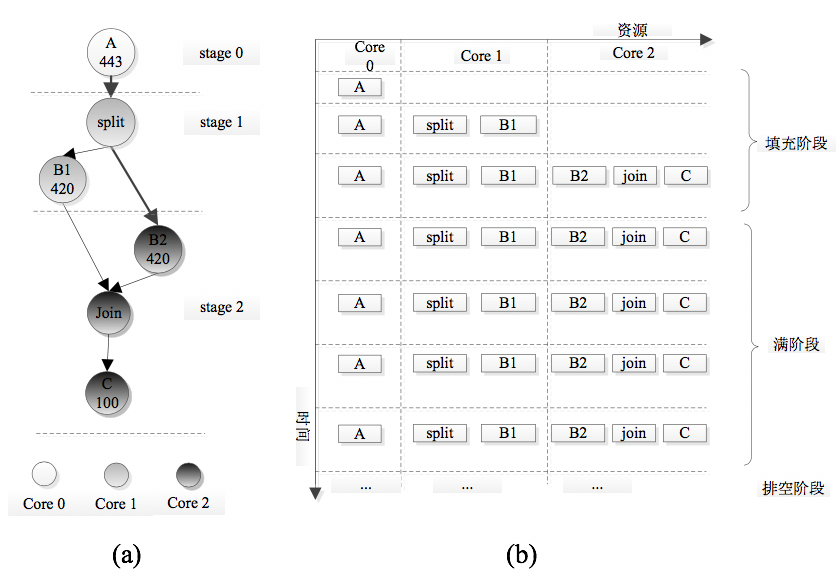
\includegraphics[width=1.0\textwidth]{Img/Chap_Application/Yu/streamline.png}\\
  \caption{(a)任务划分和阶段赋值的例子 (b)图(a)对应的软件流水执行过程}\label{fig:streamline}
\end{figure}

流水线执行过程[4]分为三个阶段,分别是填充阶段、满阶段以及排空阶段。图\ref{fig:streamline}给出了任务划分、阶段赋值和软件流水调度执行的一个例子。初始SDF图 有A、B和C这3个计算节点,在任务划分阶段将B复制分裂成两个计算单元B1和B2,同时引入了split和join两个计算节点。经过任务划分后,计算单元A被分配到处理器核core0,split和B1被分配到core1,B2、join和C被分配到core2上。图\ref{fig:streamline}(a)给出了经过阶段赋值后各个计算单元的阶段值,完成了软件流水的构造。图\ref{fig:streamline}(b)给出了对应的软件流水调度执行过程,程序启动时流水线处于填充阶段,各个核上的计算节点按照其阶段值从小到大的顺序启动执行,当所有的计算节点都启动时,流水线进入满阶段;在流水线满阶段,所有的计算节点都进行周期性的迭代执行,由于任务划分阶段基本实现了不同计算核上的负载均衡,此时核间同步开销小,资源利用率高,系统的吞吐率达到最大;在流水线调度的排空阶段,程序开始相继结束计算节点的执行,各个核的计算节点按照阶段值从小到大的顺序结束其周期性的迭代,等到所有的计算节点结束其稳态调度后,整个程序终止并释放运行时占有的各种资源。

\subsubsection{性能评估}
为了对COStream编译系统面向X86架构的编译优化进行全面的性能评估和分析,选取了11个多媒体领域常见的算法作为测试程序用COStream数据流编程语言实现作为COStream编译器的输入。
\begin{figure}[htbp]
  \centering
  % Requires \usepackage{graphicx}
  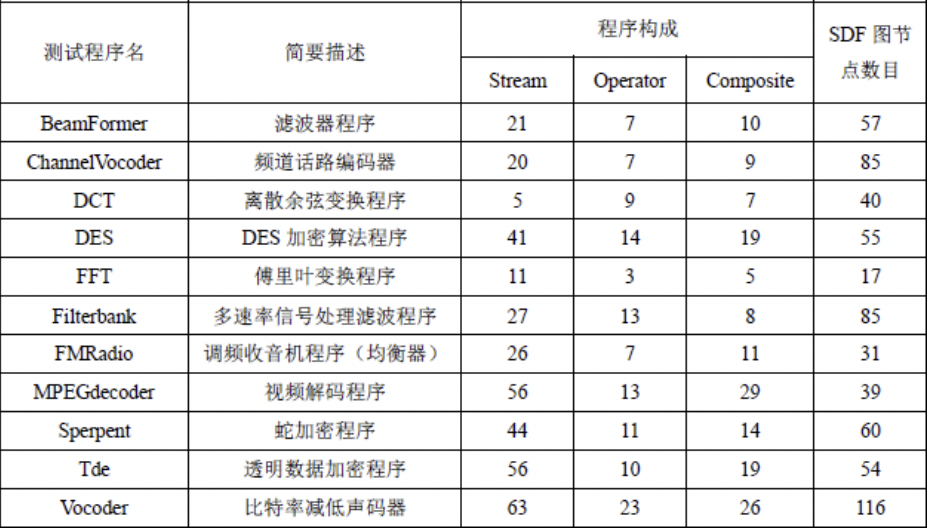
\includegraphics[width=1.0\textwidth]{Img/Chap_Application/Yu/x86benchmark.png}\\
  \caption{用于测试的数据流程序信息}\label{fig:x86benchmark}
\end{figure}

图\ref{fig:x86ratio}给出了测试程序经过COStream编译后在目标环境上执行的加速比。从图中可以看出,每个程序执行加速比随着处理核的数目增多而增加,基本呈现一个线性的加速情况。
\begin{figure}[htbp]
  \centering
  % Requires \usepackage{graphicx}
  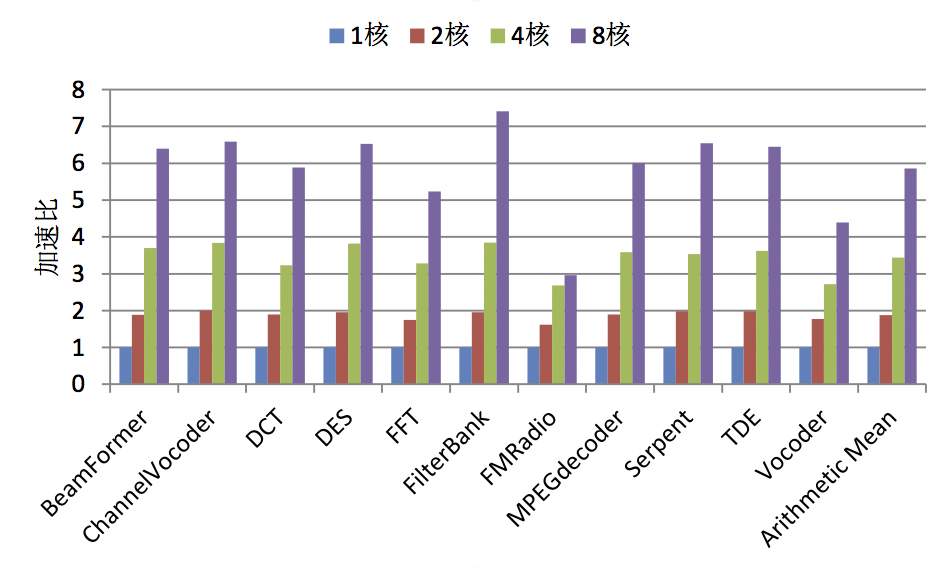
\includegraphics[width=0.8\textwidth]{Img/Chap_Application/Yu/x86ratio.png}\\
  \caption{测试代码在X86上达到的加速比}\label{fig:x86ratio}
\end{figure}

通信与同步比衡量了测试程序的有用计算和时间开销之间的比例,在一定程度上反应了程序的性能。在X86环境下采用的是软件流水调度策略,各个并行线程在软件流水调度的每次执行阶段中需要进行一次同步操作,保证不同核上的actor间的数据依赖关系能够满足。图\ref{fig:x86computeSync}给出了各个测试程序在8个核上的运行时计算同步时间分布。从图\ref{fig:x86computeSync}可以看出,FMRadio和Vocoder的计算同步比不太理想,同步开销太大,导致加速比较低,对于其他的测试程序计算同步比都能够达到较高水平,程序的加速比也较为理想。

\begin{figure}[htbp]
  \centering
  % Requires \usepackage{graphicx}
  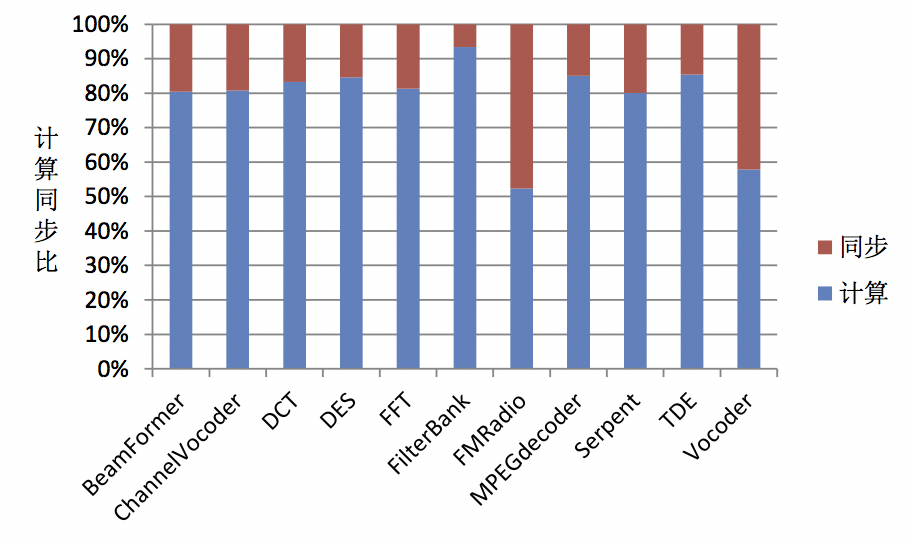
\includegraphics[width=0.8\textwidth]{Img/Chap_Application/Yu/x86computeSync.png}\\
  \caption{测试程序在8核上运行的计算同步比}\label{fig:x86computeSync}
\end{figure}

\subsection{面向 CPU 和 GPU 异构多核集群的 COStream 编译优化}

目前,各种新型的高性能体系结构不断涌现,以传统处理器CPU与图形处 理器GPU协同工作模式来构建异构硬件平台逐渐成为一种新型的并行处理方 式[1]。CPU/GPU异构集群是由多个服务器节点组成的集群,其中每个节点封装多 核CPU与一定数量的GPU。CPU/GPU异构集群相对通用CPU集群在计算、访存与通信方面存在很大的差异性,这给研究人员带来了难度。 

COStream在异构集群的数据流程序的编译优化上,提出并实现了面向 CPU/GPU混合架构的数据流程序任务划分方法和多粒度调度策略,包括任务的分类处理、GPU端任务的水平分裂和CPU端离散任务的均衡化,构造了软件流水调度,经过编译优化生成OpenCL目标代码。

GPU在大规模数据的并行方面有很大的优势,但GPU间的通信开销却相当巨大,任务划分目的主要是保证各服务器节点的计算负载均衡、通信开销最小化,以及在单个节点上,充分发挥CPU逻辑控制与串行计算特点以及GPU计算密集性优势,同时保证 CPU 多核间负载均衡和不同GPU间数据通信开销最小化。COStream在异构集群的数据流程序的编译框架中的任务划分算法主要分为任务划分预处理、任务划分与调度[10]。

\subsubsection{任务划分预处理}
该阶段主要分成两个步骤:一是引入扩大因子,二是任务的分类处理。引入扩大因子,即计算节点执行次数整体扩大,在各个应用程序中,各计算节点的执行次数远远小于GPU可并行执行的规模,采用执行次数的整体扩大的方法,增大各个计算节点的工作量,从而充分利用GPU的并行计算单元;扩大因子的上限由三个因素决定:主存大小(Host Memory)、GPU存储空间(Device Memory)和GPU缓冲区分配机制。

CPU端允许扩大倍数为N1,则
\begin{equation}
  N_1 \leq M_{CPU} / M_{CPUSumneeded} \label{eq:2.1}
\end{equation}

其中,MCPU表示主存可用空间的大小,MCPUSumneeded表示CPU端所有任务未扩大前所需的存储空间总和。

GPU端允许扩大的倍数为N2,N2需满足公式\ref{eq:2.2}和公式\ref{eq:2.3}。
\begin{equation}
  N_2 \leq M_{GPU} / M_{GPUSumneeded} \label{eq:2.2}
\end{equation}

其中,$M_{GPU}$表示GPU可用的存储空间,$M_{GPUSumneeded}$表示GPU端所有任务未扩大前所需的存储空间总和。

\begin{equation}
  N_2 \leq M_{GPU} / M_{GPUSumneeded} \label{eq:2.3}
\end{equation}

其中,$M_{GPUmaxbuffer}$表示GPU每次允许分配缓冲区的最大值,$M_{GPUmaxneeded}$表示GPU端所有任务未扩大前各需存储空间的最大值。

在同时满足公式\ref{eq:2.1}、公式\ref{eq:2.2}、公式\ref{eq:2.3}的前提下,选取合适的扩大因子为来保证GPU端任务有足够的计算量,并充分利用GPU计算资源。同时,引入扩大因子的过程间接地减少了CPU线程的同步次数,从而降低了应用程序整体的同步开销。

任务的分类处理,该步骤根据任务是否具有可并行性以及相应通信开销的大小将其分配到GPU或CPU上去运行,充分利用CPU与GPU各自的优势,同时降低整体程序的通信量。COStream数据流程序中,计算节点有两种状态:有状态(Stateful)和无状态(Stateless)。状态为Stateful的结点表示该计算结点连续两次迭代运算间存在数据依赖,两次迭代运算不可并行执行;状态为Stateless的结点则与之相反,多次换代运算之间互相独立,可并行执行。数据流程序任务的分类处理,目标是根据计算节点的计算特点,将计算节点分配到适合的计算平台上进行计算,在分类的过程中,既要考虑该计算任务是否具有可并行性,即是否为状态是Stateless的结点,同时也要考虑GPU间高额的通信开销,减小异构平台间的数据通信量。任务分类首先判断SDF图中各个计算节点的状态,将Stateless计算节点划分到GPU端,Stateful计算节点划分到CPU端。接着考虑异构平台间的通信开销,调节边界结点。对于划分到GPU端的Stateless结点,如果其父结点为Stateful结点,并且其子结点为Stateful结点,那么初步分类的结果就会带来大量的GPU间的数据通信,从而产生巨大的通信开销,影响数据流程序的整体性能,因此任务初步分类完成后,需要将此类计算节点微调到CPU端。

\subsubsection{任务划分}
基于GPU/CPU混合架构的数据流程序任务划分包括两部分内容——GPU端任务的水平分裂(GPU Tasks Horizon Splitting, GTHS)和CPU端离散任务均衡化(CPU Disperse Tasks Balancing, CDTB)。

对于任务划分,它既要满足负载均衡,又要降低通信开销,常用的针对SDF图的划分方法有METIS划分工具、K路图划分方法等。METIS划分与K路划分方法都满足负载均衡和减小通信开销的目标,由于GPU与GPU间数据通信开销的巨大,导致这两种划分方法对应用程序的整体执行效率提高不显著。

针对上述问题,GTHS算法利用任务的并行性将其均衡分裂到各GPU,以防止GPU与GPU间高额的通信开销影响数据流程序的整体性能。算法\ref{algo:gths}描述了GPU端任务水平分裂的具体实现过程,该方法主要分为两个阶段完成:一是GPU端actor的分裂,完成任务的分类处理和扩大因子的引入后,划分到GPU端的任务各自的迭代计算具有很高的并行性,但针对一些特殊的应用程序,其GPU端任务间的数据访问对前一次的运行结果有依赖性,对于这种特殊类型的应用程序不进行GPU端任务的水平分裂,而将分配到GPU端的任务均由一个GPU计算完成;该划分方法针对GPU端任务间数据访问对前一次的运行结果无依赖性的应用,遍历分配到GPU端的各actor,修改各actor的稳态执行次数,并创建M个新actor(M为GPU的个数减1),将该actor复制给M个新创建的actor(称该actor为新创建的M个actor的模板结点,新创建的M个actor为该actor的复制结点),并修改对应新结点的名字(行1-12);二是对应的新结点连接,actor分裂完成后,新创建的actor是离散的,将各离散的新创建的actor对应连接起来,形成新的连通的SDF图(行13-42)。依次遍历每一个新创建的actor,如果其模板actor的父结点是GPU端actor,则该新创建的actor的模板结点的父结点在上一阶段也进行了水平分裂,那么将该新创建的actor与其模板actor的父结点的相应复制结点连接起来;如果其模板actor的父结点是CPU端actor,则其模板actor的父结点在上一阶段未进行水平分裂,那么将该新创建的actor与其模板actor的父结点直接连接起来(行14-27);如果其模板actor的子结点是GPU端actor,则该模板结点的子结点在上一阶段也进行了水平分裂,那么需要将该新创建的actor与其模板actor的子结点的相应复制结点连接起来;如果其模板actor的子结点是CPU端actor,则该模板actor的子结点在上一阶段未进行水平分裂,那么需要将该新创建的actor与其模板actor的子结点直接连接起来(行28-41)。如图\ref{fig:3.1}所示为数据流程序GPU端任务水平分裂的结果示意图,图\ref{fig:3.1}(a)为任务的分类结果,计算节点A和计算节点F为CPU端结点计算节点B、C、D、F为GPU端结点;图\ref{fig:3.1}(b)为GPU端任务水平分裂结果,其中,计算节点A和计算节点F为CPU端结点,计算节点B1、C1、D1和E1划分到GPU0,计算节点B2、C2、D2和E2划分到GPU1,计算节点B3、C3、D3和E3划分到GPU2。

\begin{breakablealgorithm} \label{algo:gths}
  \caption{GPU端任务水平分裂算法}
  {\bf Input: GPUNode[ ], SDF graph}\\
  {\bf Output: new SDF graph}\\
  1 for all actor v in GPUNode[] do\\
  2   \hspace*{1 pc} v.executions /= GPUNumber;\\
  3   \hspace*{1 pc} int NewActorNumber = GPUNumber – 1;\\
  4   \hspace*{1 pc} int index = 1;\\
  5   \hspace*{1 pc} multimap mapActor2NewActor;\\
  6   \hspace*{1 pc} for int i = 0; i < NewActorNumber; ++i do\\
  7   \hspace*{2 pc} Actor m = CreateNewActor(v);\\
  8   \hspace*{2 pc} m.name += itoa(index);\\
  9   \hspace*{2 pc} mapActor2NewActor.insert(v,m);\\
  10  \hspace*{2 pc} ++index;\\
  11  \hspace*{1 pc} end for\\
  12end for\\
  13for all actor u in GPUNode[] do\\
  14  \hspace*{1 pc} if(IsGPUNode(u.parent))then\\
  15  \hspace*{2 pc} int index = 1;\\
  16  \hspace*{2 pc} for ;index < GPUNumber;++index do\{\\
  17  \hspace*{3 pc} Actor a = FindNewActor(u,index);\\
  18  \hspace*{3 pc} Actor b= FindNewActor(u.parent,index);\\
  19  \hspace*{3 pc} a.parent = b;\\
  20  \hspace*{2 pc} end for\\
  21  \hspace*{1 pc} else\\
  22  \hspace*{2 pc} int index = 1;\\
  23  \hspace*{2 pc} for ; index < GPUNumber; ++index do\\
  24  \hspace*{3 pc} Actor a = FindNewActor(u,index);\\
  25  \hspace*{3 pc} a.parent = u.parent;\\
  26  \hspace*{2 pc} end for\\
  27  \hspace*{1 pc} end if\\
  28  \hspace*{1 pc} if(IsGPUNode(u.child))then\\
  29  \hspace*{2 pc} int index = 1;\\
  30  \hspace*{2 pc} for ;index < GPUNumber;++index do\\
  31  \hspace*{3 pc} Actor a = FindNewActor(u,index);\\
  32  \hspace*{3 pc} Actor b= FindNewActor(u.child,index);\\
  33  \hspace*{3 pc} a.child = b;\\
  34  \hspace*{2 pc} end for\\
  35  \hspace*{1 pc} else\\
  36  \hspace*{2 pc} int index = 1;\\
  37  \hspace*{2 pc} for ; index < GPUNumber; ++index do\\
  38  \hspace*{3 pc} Actor a = FindNewActor(u,index);\\
  39  \hspace*{3 pc} a.child = u.child;\\
  40  \hspace*{2 pc} end for\\
  41  \hspace*{1 pc} end if\\
  42end for
\end{breakablealgorithm}


\begin{figure}[htbp]
  \centering
  % Requires \usepackage{graphicx}
  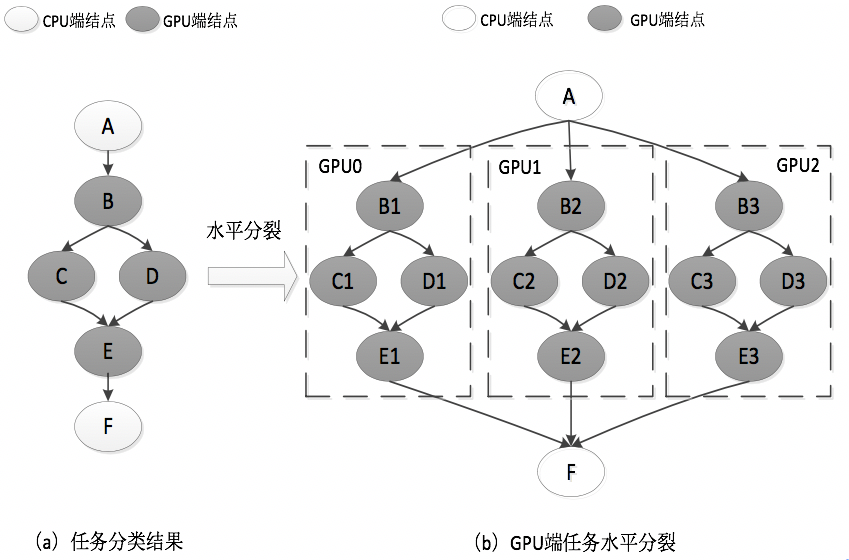
\includegraphics[width=0.8\textwidth]{Img/Chap_Application/Yu/3-1.png}\\
  \caption{GPU端任务水平分裂示意图}\label{fig:3.1}
\end{figure}


GPU/CPU混合架构平台下,GPU端任务的水平分裂完成了GPU端任务的划分,而传统的任务划分方法[9]对任务分类处理后分配到CPU端的各个离散结点未进行划分处理,均由一个CPU核控制计算,如果该CPU核的工作量过大时就会影响整个程序的执行效率。数据流程序CDTB算法针对这些CPU端的离散结点,结合复制分裂算法,选择合适CPU核,采用贪心的思想,均衡地将各计算结点分成若干个划分并将各划分映射到相应的CPU核上,保证各CPU核的负载均衡并提高各CPU核的利用率。基于GPU/CPU混合架构的数据流程序CPU端离散任务的均衡化过程主要包括以下三个阶段:

\begin{itemize}	
  \item {\bf CPU核数的确定}:图\ref{fig:3.2}为CPU核数确定过程的流程示意图。分别计算CPU端任务总的执行时间CPUTime、GPU端任务总的计算时间GPUTime以及数据流程序总的通信时间CommTime,如果CPUTime小于GPUTime和CommTime的最大值,选择CPU的核数为1,即分配到CPU端所有actor均由一个CPU核控制执行;如果CPUTime大于GPUTime和CommTime的最大值且分配到CPU端的actor个数为1,该actor的状态为stateful即该actor不可进行分裂,则选择CPU的核数为1;如果分配到CPU端的actor个数大于1或者存在工作量较大的状态为stateless的actor,根据公式\ref{eq:3.1}计算出应用程序执行时所需要的CPU核数NCPUcore;如果所求得的CPU核数大于系统可用的核数,则设置所需的CPU核数为系统可用的核数。通过CPU核数的确定,充分利用系统的计算资源,减小系统计算资源的浪费。

  \item {\bf CPU端工作量相对较大且状态为stateless的actor复制分裂}: 根据CPU端所有actor总的工作量CPUTotalWork和计算出所需的CPU核数NCPUcore,结合公式\ref{eq:3.2}求得理论上分配给每个核的最大工作量MaxTotalWork,遍历CPU端的状态为stateless的actor,根据工作量估计求出该actor的工作量大小,如果其工作量大于MaxTotalWork,则利用复制分裂算法对该actor进行复制分裂操作,将新生成的actor与其模板actor的父结点和子结点连接以保证SDF的连通性,经过多次反复的复制分裂操作使CPU端每个状态为stateless的actor的工作量都小于MaxTotalWork。
  
  \begin{equation}
    N_{CPUcore} = CPUTime/Max(GPUTime,CommTime) \label{eq:3.1}
  \end{equation}

  \begin{equation}
    MaxTotalWork = CPUTotalWork/N_{CPUcore} \label{eq:3.2}
  \end{equation}

  \item {\bf CPU端各离散的actor与CPU核间的映射}: 该过程采用贪心的思想,遍历CPU端actor并根据工作量估计计算出该actor的工作量,选择当前各自总工作量最小的CPU核,将该actor划分到当前总工作量最小的CPU核上,完成该actor与CPU核映射。算法\ref{algo:cpureflect}描述了CPU端离散任务均衡化具体过程的实现细节,该方法适合于CPU端计算成为软件流水调度过程中数据流程序整体效率瓶颈的情况。根据公式\ref{eq:3.1}和公式\ref{eq:3.2}分别计算出该应用程序所需的CPU核数NCPUcore和每个CPU核理论最大的总的工作量MaxTotalWork,遍历CPU端所有状态为stateless的actor结点,针对工作量workvalue大于MaxTotalWork的actor,通过CreateNewActor函数对该actor进行分裂操作并将新创建的actor与其模板actor的父结点和子结点连接(行1-11)。遍历所有CPU端actor,选择当前总的工作量估计最小的CPU核并完成该actor与该CPU核的映射(行12-17)。
\end{itemize}

\begin{figure}[htbp] 
  \centering
  % Requires \usepackage{graphicx}
  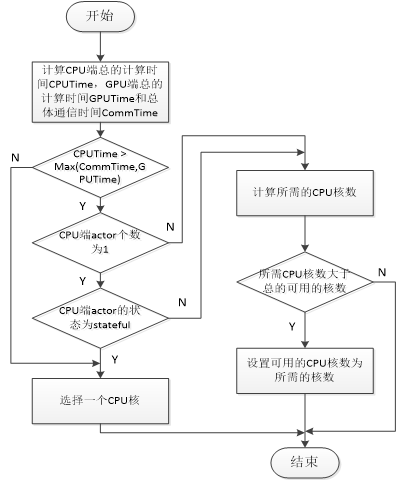
\includegraphics[width=0.8\textwidth]{Img/Chap_Application/Yu/3-2.png}\\
  \caption{CPU核数确定过程的流程示意图}\label{fig:3.2}
\end{figure}

\begin{algorithm}
  \caption{CPU端离散任务均衡算法}
  \label{algo:cpureflect}
  Input: CPUNode[]\\
  Output: mapActor2Partition(actor:partition)\\
  for( all actor v in CPUNode[] ) \{\\
    \hspace*{1 pc} int workvalue = CalculateWorkValue(v);\\
    \hspace*{1 pc} if(!DetectiveActorState(v) \&\& workvalue > MaxTotalWork)\{\\
    \hspace*{2 pc} int number = workvalue / MaxTotalWork;\\
    \hspace*{2 pc} for(int i = 0; i < number; ++i) \{\\
    \hspace*{3 pc} Actor u = CreateNewActor(v);\\
    \hspace*{3 pc} u.parent = v.parent;\\
    \hspace*{3 pc} u.child = v.child;\\
    \hspace*{2 pc} \}\\
    \hspace*{1 pc} \}\\
  \}\\
  for( all actor w in CPUNode[] )\{\\
    \hspace*{1 pc} int workvalue = CalculateWorkValue(w);\\
    \hspace*{1 pc} int index = FindMinWorkvalueCore();\\
    \hspace*{1 pc} UpdateWorkvalue(index);\\
    \hspace*{1 pc} mapActor2Partition(w:index);\\
  \}
  \end{algorithm}

\subsubsection{阶段赋值}
基于GPU/CPU混合架构的数据流程序优化框架采用软件流水调度方式,主要解决了软件流水调度过程中的三个问题:

\begin{itemize}	
  \item {\bf 线程同步问题}:在软件流水调度[8]过程中,每个线程执行完各自的计算任务后,都需要进行一次同步操作[11],保证各个线程处于同一调度阶段,虽然该同步开销比硬件调度方式下的同步开销小,但由于计算任务的工作量过小或者处理器核数的增加都有可能带来同步开销的增大,从而影响了应用程序的执行效率。该优化框架引入扩大因子,成倍的扩大计算任务的稳态执行次数,增大各个计算任务的工作量,使计算任务多次计算后,同步一次,从而大大地减小了程序的同步操作数,增加了计算同步比,同时也充分利用了GPU/CPU混合架构下GPU高度并行计算的优势,提高了数据流程序的执行效率。

  \item {\bf 负载均衡问题}: 软件流水调度过程中,负载均衡是影响应用程序整体执行效率的重要因素。在GPU/CPU混合架构系统平台下,由于GPU与CPU计算能力的不对等,如果各个线程的负载不均衡,则会带来多个线程忙等的现象,增加程序的同步开销。该优化框架通过GPU端任务水平分裂算法和CPU端离散任务均衡化算法,实现了GPU端计算、CPU端计算和异构通信的相对均衡,同时降低了应用程序的通信量。
  
  \item {\bf 通信开销问题}: 在GPU/CPU混合架构中,异构通信占用软件流水调度的一个阶段,达到软件流水满状态,即计算任务稳态执行阶段,CPU端任务的计算、GPU端任务的计算以及CPU与GPU间的数据通信是并行执行的,高额的通信开销也会降低应用程序的执行效率。该优化框架采用任务分类方法,结合任务的计算特点,完成任务的分类,同时也降低异构的通信开销;GPU端任务的水平分裂,将GPU端任务均衡分裂到各GPU,避免了GPU与GPU间的高额通信,达到降低通信开销的目的。
\end{itemize}

经过GPU端GTHS算法和CPU端CDTB算法的任务划分,SDF图中的actor均被划分到对应的计算单元上运行,挖掘状态为stateful类型的结点的流水线并行性,构造软件流水线调度,使得状态为stateful的结点连续两次迭代计算,结点计算和数据传输都可以重叠执行,需要确定各结点被流水调度执行时的阶段号,即进行阶段赋值。

\begin{algorithm}
  \caption{基于GPU/CPU混合架构的阶段赋值}
  \label{algo:gpucpu}
  Input: SDFgraph, CPUNode[],GPUNode[], mapActor2Partition(actor:partition)\\
  Output: mapActor2Stage(actor:stage)\\
  TopologyOrderofActors = TopologyTravSDF();\\
  int MaxStage = 0;\\
  int tempStage;\\
  for all actor v in TopologyOrderofActors \{\\
    \hspace*{1 pc} for all actor u which is parent of v \{\\
    \hspace*{2 pc} if((IsCPUNode(v) \&\& IsCPUNode(u)) || IsGPUNode(v) \&\& IsGPUNode(u))\{\\
    \hspace*{3 pc} if(mapActor2Partition[v] == mapActor2Partition[u])\{\\
    \hspace*{4 pc} tempStage = mapActor2Stage[u];\\
    \hspace*{3 pc} \}else\{\\
    \hspace*{4 pc} tempStage = mapActor2Stage[u] + 1;\\
    \hspace*{3 pc} \}\\
    \hspace*{2 pc} \}else\{\\
    \hspace*{3 pc} tempStage = mapActor2Stage[u] + 2;\\
    \hspace*{2 pc} \}\\
    \hspace*{2 pc} if(tempStage > MaxStage)\{\\
    \hspace*{3 pc} MaxStage = tempStage;\\
    \hspace*{2 pc} \}\\
    \hspace*{1 pc} \}\\
    \hspace*{1 pc} mapActor2Stage[v] = MaxStage;\\
  \}
\end{algorithm}

算法\ref{algo:gpucpu}描述了面向GPU/CPU混合架构的数据流程序阶段赋值过程。对SDF图进行拓扑排序以满足数据的读写规则(行1),依次遍历拓扑排序中的各actor,如果该actor与其父结点同在CPU端或同在GPU端,并且属于同一个划分,那么该actor阶段号与其父结点阶段号相同;如果该actor与其父结点同在CPU端或同在GPU端,但是不属于同一个划分,那么该actor阶段号等于其父结点阶段号加1;如果该actor与其父结点不同在CPU端或GPU端,那么该actor阶段号等于其父结点阶段号加2(行4-21),因为该actor与其父结点不同在CPU端或不同在GPU端则会产生通信,数据通信在软件流水调度过程中需要占用一个阶段号。图\ref{fig:gpucpu}所示为基于GPU/CPU混合架构的阶段赋值结果,其中,actor A、B、C为CPU端结点,actor D、E、F、G、I为GPU端结点,在CPU端,actor A为一个划分,actor B和C属于同一个划分,actor A的阶段号为0,actor B与actor A都是CPU端结点,但不属于同一划分,根据算法\ref{algo:gpucpu},actor B的阶段号为actor A的阶段号加上1;actor C和actor B都是CPU端结点,并且属于相同的划分,因此,actor C的阶段号等于actor B的阶段号;actor D与actor C分配在不同的平台,即不同在GPU或CPU,actor D的阶段号为actor C的阶段号加上2,因为actor C与actor D的数据通信需要占用一个阶段号,由于GPU的并行规模比较丰富,实验中将分配到GPU并且连通的结点划分同一个阶段执行。


\begin{figure}[htbp]
  \centering
  % Requires \usepackage{graphicx}
  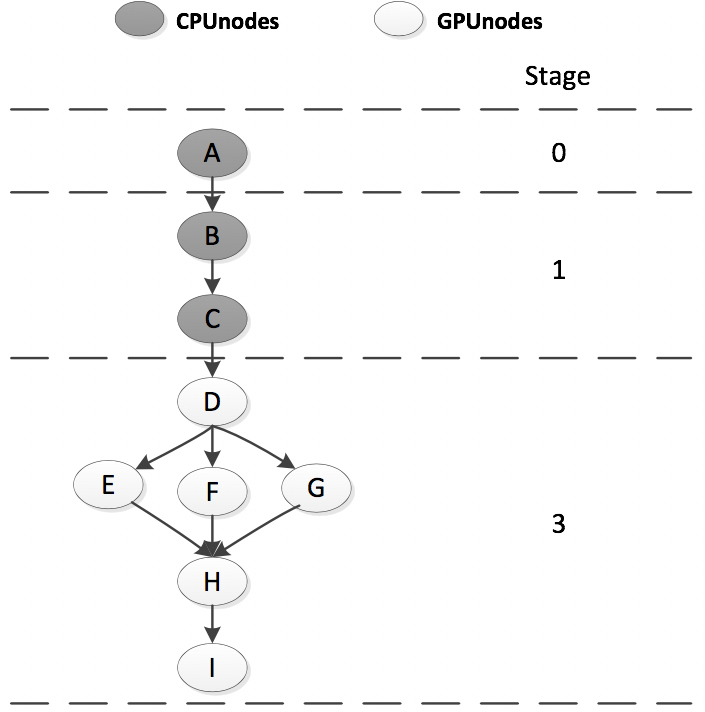
\includegraphics[width=0.8\textwidth]{Img/Chap_Application/Yu/gpucpu.png}\\
  \caption{基于GPU/CPU混合架构的阶段赋值}\label{fig:gpucpu}
\end{figure}

在三块NVIDIA Tesla C2050、两块四核CPU为混合架构系统结构上进行测试(图\ref{fig:fusion})。选取9个数字多媒体领域的典型算法作为测试程序。

\begin{figure}[htbp]
  \centering
  % Requires \usepackage{graphicx}
  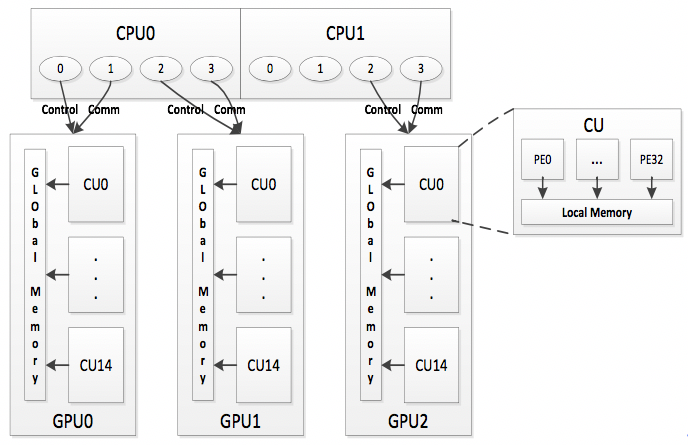
\includegraphics[width=0.8\textwidth]{Img/Chap_Application/Yu/fusion.png}\\
  \caption{混合架构系统结构}\label{fig:fusion}
\end{figure}

图\ref{fig:gm-commu}和图\ref{fig:gths-metis}显示了比较GPU端任务水平分裂算法与通用METIS划分算法的通信量以及执行时间的结果。可见在GPU/CPU混合架构平台下GTHS算法的执行效果优于METIS划分方法。

\begin{figure}[htbp]
  \centering
  % Requires \usepackage{graphicx}
  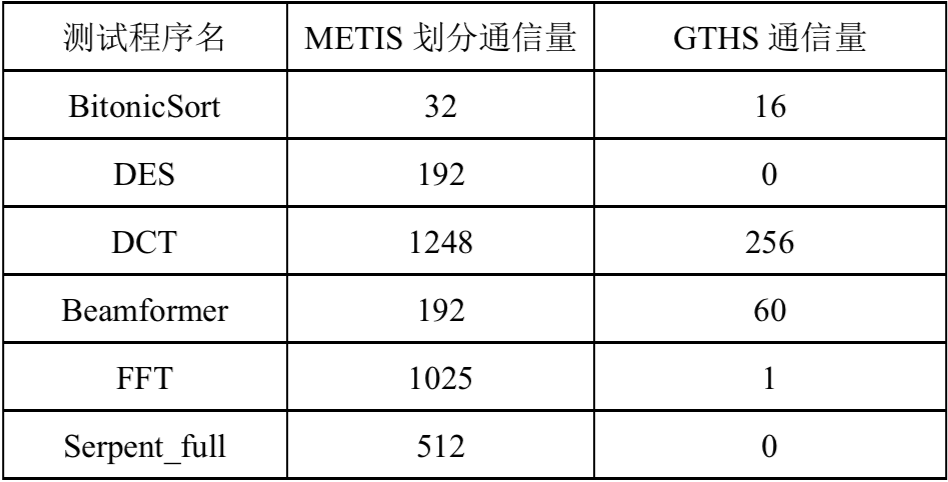
\includegraphics[width=0.8\textwidth]{Img/Chap_Application/Yu/gths-metis-commu.png}\\
  \caption{GTHS与METIS划分通信量比较}\label{fig:gm-commu}
\end{figure}

\begin{figure}[htbp]
  \centering
  % Requires \usepackage{graphicx}
  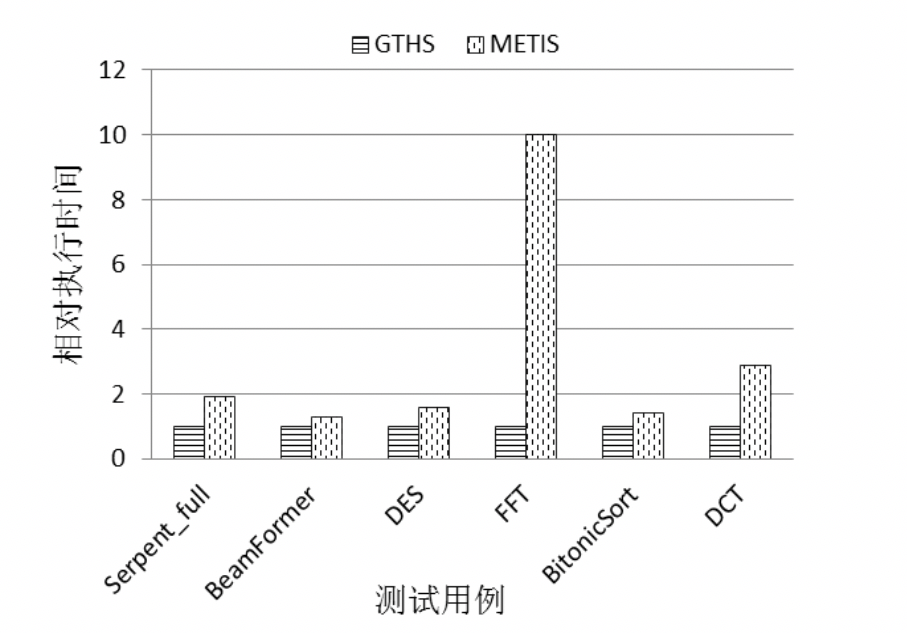
\includegraphics[width=0.8\textwidth]{Img/Chap_Application/Yu/gths-metis.png}\\
  \caption{GTHS与METIS划分执行性能比较}\label{fig:gths-metis}
\end{figure}

对于CPU端任务较重的情况采用CDTB方法进行任务划分,比较CPU端离散任务均衡化算法与传统CPU端单核计算的执行时间。可见CDTB方法更适合于CPU端任务较重且状态为stateful的actor的计算量较小的应用程序。

在GPU/CPU混合架构平台上,采用CPU与GPU协作计算的模式,充分发挥各计算单元的优势,CPU负责控制主程序的流程和串行计算,准备GPU端计算所需的相应的数据并将其传输给GPU,充分利用GPU进行高效的并行计算。图\ref{fig:5.4}为数据流程序分别采用CPU单核和1个GPU协作计算的模式与CPU单核计算并执行1000次的性能比较示意图,测试程序Beamformer中存在大量离散的状态为stateful的结点,导致执行过程中产生大量的CPU与GPU的数据通信,高额的数据通信开销使程序的性能只提高6.8,相对加速效果不明显。而对于测试程序FFT和ChannelVocoder,程序内部的通信开销相对GPU的计算开销很小,充分利用了GPU强大的并行计算规模,所以加速效果显著。

\begin{figure}[htbp]
  \centering
  % Requires \usepackage{graphicx}
  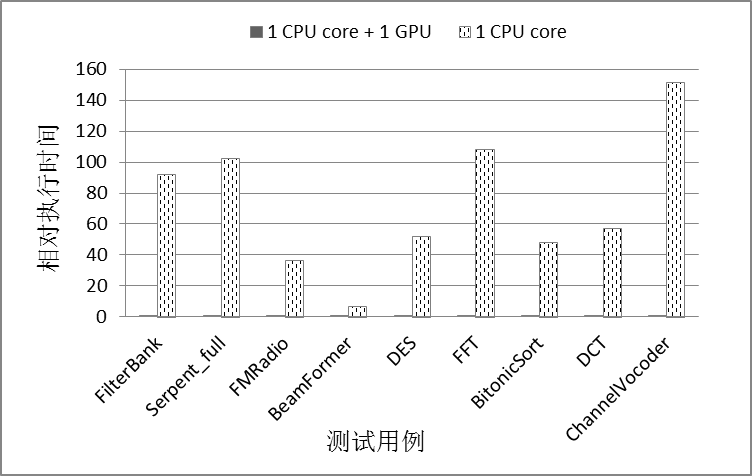
\includegraphics[width=0.8\textwidth]{Img/Chap_Application/Yu/5-4.png}\\
  \caption{CPU与GPU协作计算相对CPU单核的性能比较}\label{fig:5.4}
\end{figure}

图\ref{fig:3gpu-1gpu}所示为数据流程序分别采用三个GPU与一个GPU并执行1000次的执行性能的比较示意图。从图中可以看出,对于测试用例BeamFormer和BitonicSort,CPU端任务计算量较重,远远大于GPU端的运行时间,采用三个GPU进行并行计算,相对于采用一个GPU计算的加速效果不明显。而对于测试用例Serpent\_full和DES,CPU端任务计算量较轻,远小于GPU端任务的计算时间,采用三个GPU并行计算的加速效果比较显著。

\begin{figure}[htbp]
  \centering
  % Requires \usepackage{graphicx}
  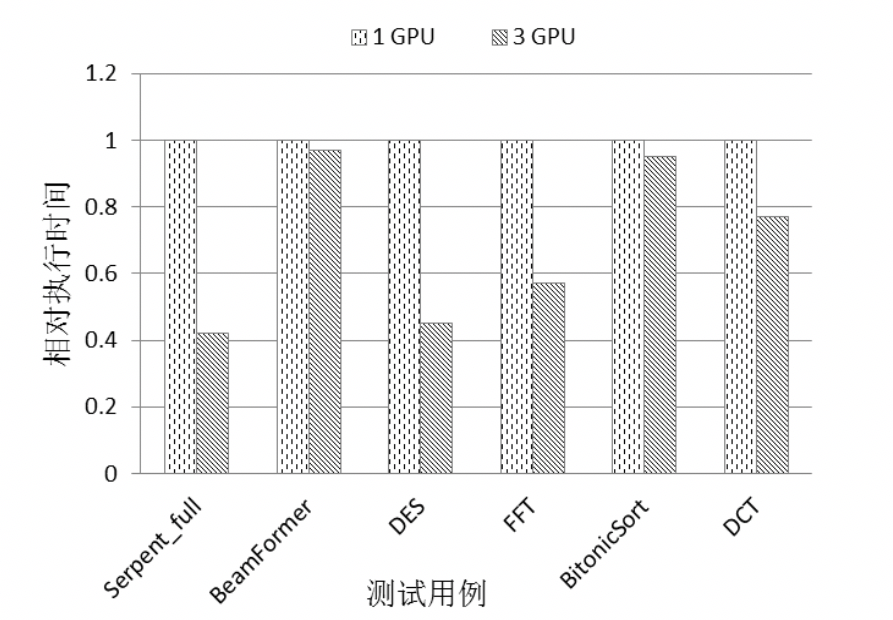
\includegraphics[width=0.8\textwidth]{Img/Chap_Application/Yu/3gpu-1gpu.png}\\
  \caption{三个GPU与一个GPU执行性能比}\label{fig:3gpu-1gpu}
\end{figure}

\subsection{基于 COStream 的深度学习程序开发实例}

深度学习模型本质是数学模型,在基于COStream实现深度学习模型时,只要将深度学习中的数学逻辑拆分成独立的计算节点并明确它们之间的数据依赖关系,其实不难实现。神经网络由神经元组成,在设计神经网络时,需要考虑网络的整体结构,应该有多少神经元,以及这些神经元应该如何相连。大多数神经网络被组织成称为层的单元组,如全连接层、卷积层等,不同类型的层连接方式不同,大多数神经网络将这些层布置成链式结构。后文将按照层来拆分整个网络模型。

神经网络模型的训练主要有两个阶段,正向传播和反向传播。尽管深度学习中每一类层对应的计算节点的数学逻辑不同,但是其正向传播和反向传播对应的计算节点的输入流和输出流遵循相同的规则。

对于正向传播,其计算过程是多个函数的复合,假设模型中每一层对应的函数依次为$f^{\left (1 \right )}$、$f^{\left (2 \right )}$、$f^{\left (3 \right )}$、$f^{\left (4 \right )}$,则复合成一条$f\left ( x \right )= f^{\left (4 \right )}\left ( f^{\left (3 \right )}\left ( f^{\left (2 \right )}\left ( f^{\left (1 \right )}\left ( x \right ) \right ) \right ) \right )$的计算链,其中x代表输入层的输入,相邻层之间存在数据依赖,形成流水线。

对于反向传播,其计算过程也是多个函数的复合,利用链式求导法则,按照网络模型反向逐层计算并传递误差(由于正向传播和反向传播计算过程中层的计算顺序是相反的,因此在下文中将始终按照网络模型中定义的层间关系来表述),需要分别计算该层参数和该层输入关于损失函数的偏导数,该计算依赖于模型中该层下一层传入的输入误差、正向传播时该层的输入值和参数矩阵。最终,根据误差更新参数。

正向传播和反向传播各层间在时间维度上是串行关系,可以用数据流编程模型提供的软件流水线并行方式进行处理。

对于模型中的参数,由于计算除依赖于上一个计算节点输出的数据流,还依赖于网络模型中的随着计算迭代更新的参数,因此将各层节点的参数定义为全局变量。

因此,层的正向传播阶段计算节点有且仅有一条输入流,数据流内为上一层正向传播阶段计算节点的输出或由训练集数据;有两个输出流,将计算结果分别传递给下一层对应的正向传播和反向传播计算节点。层在反向传播阶段的计算节点有两个输入流,其一为下一层反向传播阶段计算节点计算的误差,其二为正向传播过程中传入该层的输入;有一个输出流,将该层计算的误差继续传递上一层反向传播阶段的计算节点。

对于一个包含三个层的神经网络,它的数据流图如图\ref{fig:dataflow_graph_of_net_with_3_layers}。
\begin{figure}[!t]
\centering
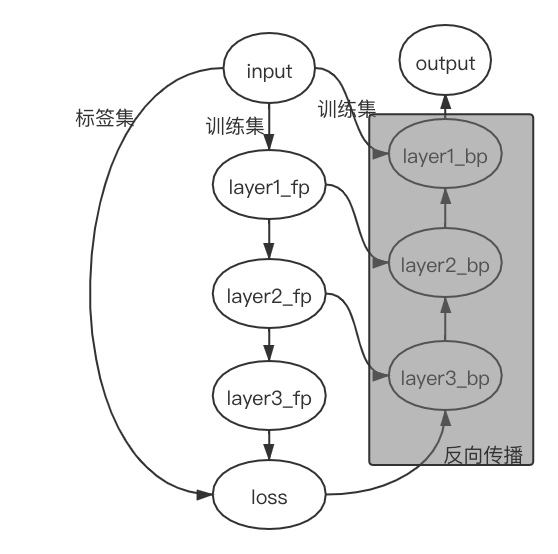
\includegraphics[width=0.8\textwidth]{../img/Chap_Application/Yu/dataflow_graph_of_net_with_3_layers.png}
\caption{包含三个层的神经网络的数据流图}
\label{fig:dataflow_graph_of_net_with_3_layers}
\end{figure}

接下来选用MNIST数据集,其训练集是由来自 250 个不同人手写的数字构成的单通道$28\ast28$图片,分别设计全连接神经网络和卷积神经网络解决识别手写数字的问题。

\subsubsection{全连接神经网络的并行化分析与设计}
全连接神经网络由全连接层组成,全连接层中的每一个神经元都与上一层中所有神经元相连,神经元将输出它所在层的上一层中所有与其相连的神经元同相连边上权值相乘后累加的结果,若对该层设置了激活函数,如ReLU函数、Sigmoid函数等,则该层中所有神经元将输出上述累乘求和结果关于该激活函数的映射,如图\ref{fig:neure}。因此,全连接层用来将该层之前的层提取到的特征综合起来。

\begin{figure}[!t]
\centering
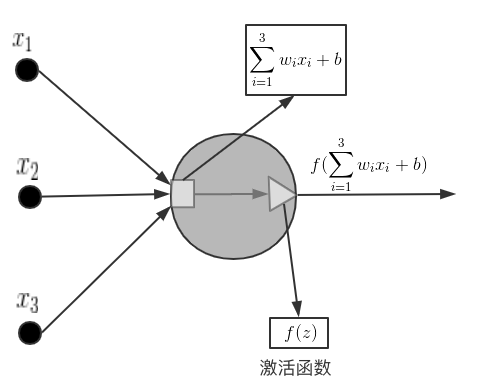
\includegraphics[width=0.7\textwidth]{../img/Chap_Application/Yu/neure.png}
\caption{神经元}
\label{fig:neure}
\end{figure}

现在基于MNIST数据集解决手写数字识别问题,由于数据集中单张图片的像素数为784($28\ast28$),所以输入层的神经元个数为784,设计该全连接神经网络共包含四层全连接层,其中前三层每层包含20个神经元,最后一层神经元的数量为10,依次对应手写图片为数字0到9预测概率。图\ref{fig:dnn}为该全连接神经网络模型。

\begin{figure}[!t]
\centering
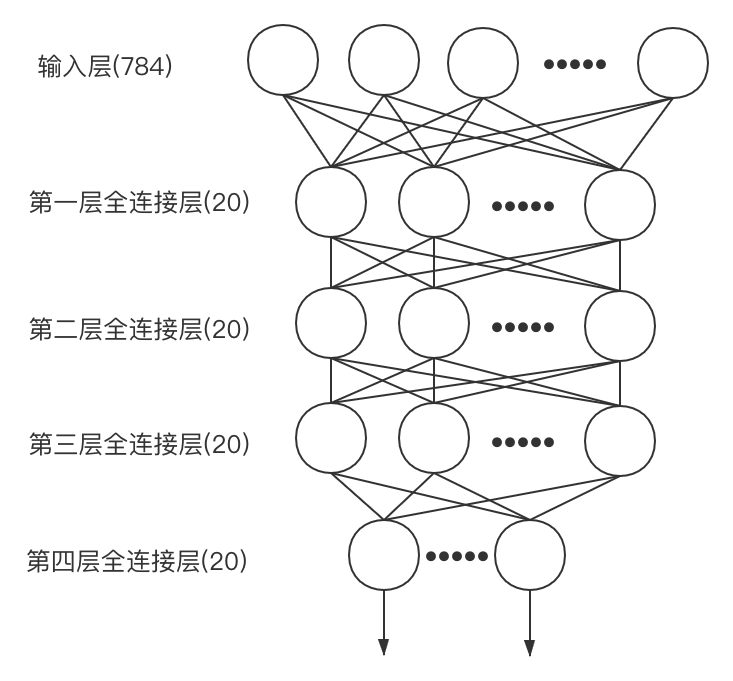
\includegraphics[width=0.8\textwidth]{../img/Chap_Application/Yu/dnn.png}
\caption{四层全连接神经网络}
\label{fig:dnn}
\end{figure}

全连接层正向传播过程执行的计算实际为向量乘矩阵运算,即传入第i层的数据构成的向量$h^{i - 1}$乘第i层参数构成的矩阵$W^{i}$,对于首层全连接层$h^{0}$等于训练集${x}$。向量矩阵运算可以被拆分成多个向量乘法运算,也即将全连接层拆分成以神经元为单位的粒度更小的计算节点,不难发现拆分后实现的计算节点间没有数据依赖关系,可以并行地执行。

根据链式求导法则,全连接层反向传播的过程也是矩阵乘法,因此同样可以用正向传播中图节点代表神经元的方式对该层进行数据并行处理。

为了验证COStream对该全连接神经网络模型并行化实现的有效性,选择了IBM-3650服务器作为实验平台进行测试,该服务器是Intel平台的x86-64架构服务器,拥有2个4核的Intel Xeon E5420 CPU,CPU主频为2.50GHz,内存的容量是8GB,最大支持48GB,硬盘容量672GB。实验平台使用的操作系统是Ubuntu16.04,系统的内核版本为4.15.0,编译器所使用的gcc版本为5.4.0,g++版本为5.4.0。经测试如图\ref{fig:dnn_speedup},根据上述方法实现的全连接网络在不同CPU核数下均表现出良好的并行加速效果。

\begin{figure}[!t]
\centering
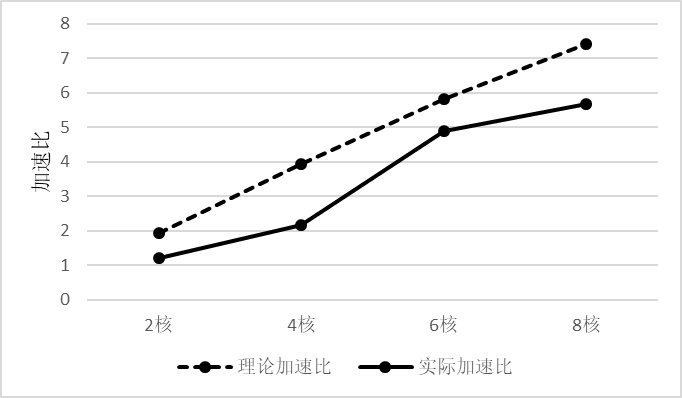
\includegraphics[width=0.8\textwidth]{../img/Chap_Application/Yu/dnn_speedup.png}
\caption{示例全连接神经网络多核加速比}
\label{fig:dnn_speedup}
\end{figure}

\subsubsection{LeNet-5 卷积神经网络的并行化分析与设计}

卷积神经网络是一种专门用来处理具有类似网格结构的数据的神经网络,例如图像数据(可以看作二维的像素网格),在卷积网络中至少有一层使用了卷积运算来替代上述全连接层中矩阵乘法运算的神经网络。

一个典型的卷积网络中通常包含三种简单层,在第一层卷积层,并行地计算多个卷积产生一组线性激活响应。在第二层探测层,每一个线性激活响应将会通过一个非线性的激活函数。在第三层池化层中,调用池化函数,它使用某一位置的相邻输出的总体统计特征来替代网络在该位置的输出。值得注意的是,只有卷积层拥有参数。

基于MNIST数据集设计如图\ref{fig:cnn}所示的卷积神经网络解决手写数字识别问题。

\begin{figure}[!t]
\centering
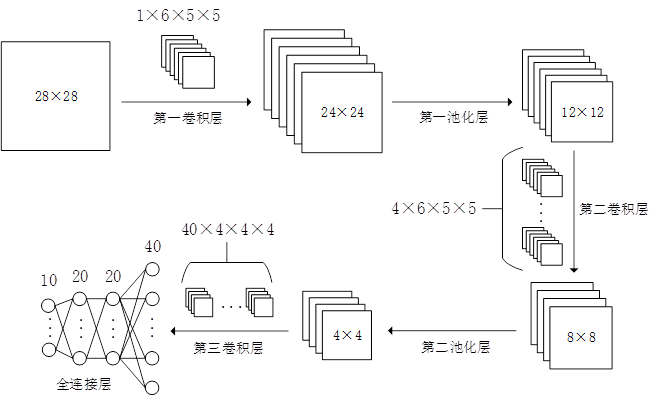
\includegraphics[width=0.8\textwidth]{../img/Chap_Application/Yu/cnn.png}
\caption{卷积神经网络}
\label{fig:cnn}
\end{figure}

对于卷积层,首先每一层通常包含多个卷积核,由于每个卷积核对应的卷积操作是相互独立的,因此可以卷积层按照卷积核数拆分成多个卷积操作,其次,每个卷积核对应多通道,通道间的卷及操作同样是相互独立的,因此可以继续将上述卷积操作继续拆分成对输入的每个通道的卷积操作$conv\_kernel$。此时,卷积层的计算由多个更细粒度的卷积操作构成,可以利用splitjoin结构按照如图\ref{fig:cnn_conv_layer}来实现,先将输入复制分发给每个卷积核,再将输入按照通道逐一分发给对应通道的卷积核。
\begin{figure}[!t]
\centering
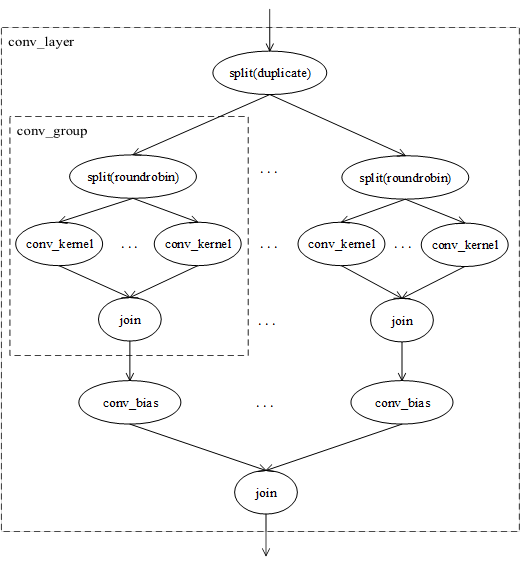
\includegraphics[width=0.8\textwidth]{../img/Chap_Application/Yu/cnn_conv_layer.png}
\caption{卷积层模块中composite间的结构关系示意图}
\label{fig:cnn_conv_layer}
\end{figure}

对于池化层,将输入按照不同通道做池化操作,同样利用splitjoin结构来实现,如图\ref{fig:cnn_pooling_layer}。

\begin{figure}[!t]
\centering
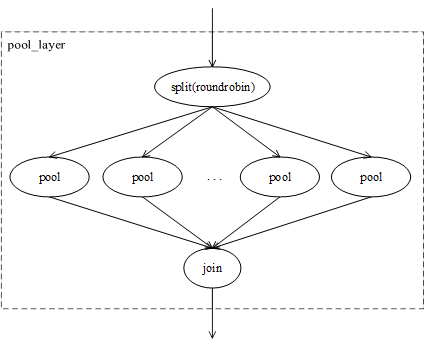
\includegraphics[width=0.8\textwidth]{../img/Chap_Application/Yu/cnn_pooling_layer.png}
\caption{池化层模块中composite间的结构关系示意图}
\label{fig:cnn_pooling_layer}
\end{figure}

\begin{figure}[!t]
  \centering
  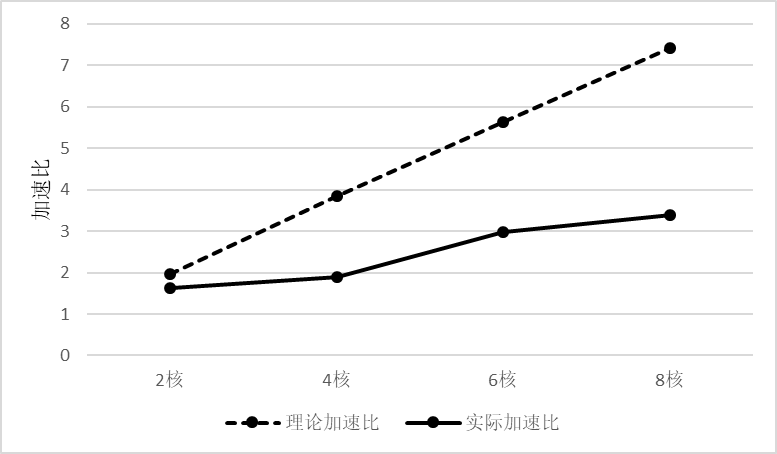
\includegraphics[width=0.8\textwidth]{../img/Chap_Application/Yu/cnn_speedup.png}
  \caption{示例卷积神经网络多核加速比}
  \label{fig:cnn_speedup}
\end{figure}

为了验证COStream对该卷积神经网络模型并行化实现的有效性,选择了IBM-3650服务器作为实验平台进行测试,该服务器是Intel平台的x86-64架构服务器,拥有2个4核的Intel Xeon E5420 CPU,CPU主频为2.50GHz,内存的容量是8GB,最大支持48GB,硬盘容量672GB。实验平台使用的操作系统是Ubuntu16.04,系统的内核版本为4.15.0,编译器所使用的gcc版本为5.4.0,g++版本为5.4.0。经测试如图\ref{fig:cnn_speedup},根据上述方法实现的卷积网络在不同CPU核数下均表现出一定的并行加速效果。


\subsection{相关工作}

\subsection{参考文献}
[1]魏海涛. 面向多核处理器的数据流程序编译关键技术研究(博士论文), 华中科技大学,2010.\\

[2] 张维维, 魏海涛, 于俊清, 李鹤, 黎昊, 杨秋吉. COStream:一种面向数据流的编程语言和编译器实现, 计算机学报, 2013, 36(10):1993 -2006

[3] Haitao Wei, Mingkang Qin, Junqing Yu, Dongrui Fan and Guang R. Gao. StreamTMC: Stream Compilation for Tiled Multi-core Architectures, Journal of Parallel and Distributed Computing (JPDC), 2013, 73(4): 484-494

[4] Haitao Wei, Junqing Yu, Huafei Yu, Mingkang Qin and Guang R. Gao. Software Pipelining for Stream Programs on Resource Constrained Multi-core Architecture, IEEE Transactions on Parallel and Distributed Systems, 2012, 23(12): 2338-2349

[5] Haitao Wei, Junqing Yu, Huafei Yu, Guangrong Gao. Minimizing Communication in Rate-Optimal Software Pipelining for Stream Programs, The 8th International Symposium on Code Generation and Optimization (CGO), 2010,Toronto, Canada, 210~217

[6] 魏海涛, 秦明康, 于俊清,范东睿. 一种面向众核架构的数据流编译框架, 计算机学报, 2014, 37(7): 1560-1569)

[7] 于俊清, 余华飞, 魏海涛, 秦明康. 多核环境下编译器辅助消息驱动的动态调度, 计算机学报, 2014, 37(7): 1633-1637

[8] 于俊清, 张维维, 陈文斌, 涂浩, 何云峰. 面向多核集群的数据流程序层次流水线并行优化方法研究, 计算机学报, 2014, 37(10): 2071-2083

[9] 魏海涛, 于俊清, 余华飞, 秦明康. 一种面向数据流程序的软件流水并行化方法, 计算机学报, 2011, 34(5): 889~898)

[10] 陈文斌,杨瑞瑞,于俊清. 基于GPU/CPU混合架构的流程序多粒度划分与调度方法研究, 计算机工程与科学,2017, 39(1): 15-26)

[11] 杨胜哲, 于俊清, 唐九飞. 数据流程序动态调度与优化方法研究, 计算机工程与科学,2017, 39(7): 1201-1210)

[12] 唐九飞, 李 鹤, 于俊清. 面向X86多核处理器的数据流程序任务调度与缓存优化, 中国科学技术大学学报, 2016, 46(3): 200-207

[13] 王兆吉. 利用COStream实现全连接和卷积神经网络的并行计算(硕士论文),2019,华中科技大学

\section{数据流编程理论与模型在类脑计算中的应用}
\subsection{引言}
近年来,借鉴人脑信息处理模式和结构的类脑计算得到了长足发展。类脑计算中最常用的计算模型是脉冲神经网络(spiking neural network,SNN),结合SNN与深度神经网络(deep neural network,DNN)各自优势的相关研究工作[天机芯片,nature]也正逐渐展开。

SNN网络的执行过程具有事件驱动、异步并发、活动稀疏性等特点,直观上较为符合数据流执行模型的特点,因此以数据流编程理论与模型为指导,进行类脑计算的SNN网络软件仿真与硬件芯片优化设计是题中应有之义。

本章就以下几方面问题开展了研究介绍,第一是数据流模型启发下的支持DNN特性的通用SNN描述语言,该语言针对SNN与DNN相融合的研究趋势,扩展了目前较为主流的SNN描述语言PyNN,是其能够支持DNN的描述需求;第二是面向GPGPU的SNN模拟,;最后是基于数据流模型有效指导类脑芯片结构设计,包括两个主要内容,即数据流模型指导下的神经网络编译以及与该编译技术对应的基于RRAM(阻变存储器)交叉开关结构的可重构神经网络加速器设计。

(包括一张图给出这几个方面的层次关系)


\subsection{支持DNN特性的通用SNN描述语言(计划替换为该内容)}
(1)通用SNN描述语言的研究背景与动机\\
SNN是目前类脑计算采用的主要计算模型,DNN则是目前机器学习领域广泛应用的计算模型,随着双方研究工作的进展,SNN和DNN开始出现相互借鉴乃至逐步融合的趋势。SNN与DNN在神经元和突触模型、网络描述方式、信息传输模式和训练算法等方面存在的差异,使得现存的SNN描述语言并不支持DNN特性。因此一种通用 SNN 描述语言——支持DNN特性的SNN描述语言将在以下方面起到积极促进作用:

\begin{itemize}
    \item 训练算法:可以提高将DNN优秀的学习算法移植到SNN的效率。当前相关的工作往往要求使用者同时具有DNN(计算机和人工智能领域)和SNN(生物和脑科学领域)的相关背景,并能够熟练地使用两方面的相关工具。通用SNN描述语言可以减轻SNN开发人员对DNN相关背景知识和工具的依赖,使得他们在使用SNN同时,能够便捷地利用DNN领域的训练算法。
    \item 应用领域:目前,相当一部分神经形态芯片支持使用SNN语言进行应用开发(例如 BrainScaleS[8]和SpiNNaker[9]系统支持广泛使用的SNN描述语言PyNN[29])。通用SNN 描述语言可以将基于DNN的机器学习应用便捷地移 植到上述神经形态硬件平台,从而拓展上述硬件平台的应用领域。 
    \item 执行效率:部分神经形态芯片采用了异步电路设计以更加契合SNN的计算模型,从而极大地降低了芯片的功耗[30]。通用SNN描述语言有助于建立针对神经形态硬件的开发工具链,从而可以在上述平台上直接开发机器学习相 关应用,提高机器学习应用的执行性能并减少总体功耗。 
    \item 资源共享:尽管目前SNN和DNN相互借鉴甚至融合的趋势已经初步显现,但两者在神经元和突触模型、网络描述方式、训练算法,和信息传输模式层面的不同严重阻碍了双方社区的资源共享和互相合作。上述领域专用语言将有助于SNN共同体和DNN共同体的资源共享。

\end{itemize}

(2)SNN描述语言——PyNN\\

随着类脑计算的发展,出现了越来越多支持SNN 的计算平台,诸如SNN模拟器[11,12,15],神经形态芯片[8,9] 以及FPGA系统[32] 等。为提高SNN模型的可移植性和通用性,多种独立于模拟器的SNN描述语言(例如PyNN[29]和SpineML[51])得到了越来越广泛的应用。其中基于Python的领域专用语言PyNN,得到了众多 SNN模拟器(例如 NeMo[14],NEST[11],PCSIM[12],Brian[15]和Brian21 O[31])、众多神经形态芯片(例如BrainScaleS[8]和SpiNNaker[9])以及FPGA系统(例如NeuroFlow[32])的支持。通常情况下,PyNN 使用高层次的抽象模型(神经元组成的集群和它们之间的连接)描述SNN,提供了多种标准的神经元和突触模型,以及一系列的连接算法。

PyNN是一种基于Python的领域专用语言。用户可以使用PyNN构建基于Python代码的SNN模型,并可以在任意支持PyNN的模拟器上运行。PyNN的具体实现是一个由通用模块(包含标准的神经元、突触模型,以及一系列广泛使用的连接算法)和针对不同模拟器后端的专用模块组成的Python 包。PyNN 提供了一个面向对象的编程接口,可以在神经元集群和突触映射的层面描述 SNN。PyNN 的具体后端实现则可以将上层的 SNN 描述和底层模拟器实现的具体函数接口连接起来。因此,PyNN 语言本身仅仅提供了对 SNN 的高层次描述方法,具体的执行性能由后端实现决定。部分支持PyNN的模拟器实现(例如 Brian[15])通过代码生成来实现对使用PyNN描述的神经网络的高效执行。PyNN的核心语言类型如下:

\begin{itemize}
    \item 神经元类型。PyNN中所有的神经元类型都是类BaseCellType的子类。神经元对应的参数可以在实例化的同时进行设置,且不同的神经元模型都继承了相同的基本操作函数。PyNN中定义了多个常用的神经元类型(例如 IF\_curr\_exp, IF\_curr\_alpha等),这些神经元类型在不同的后端实现中都具有统一的计算实现。 PyNN中定义的神经元相应的计算类似 DNN 中的激活函数,PyNN 的原始定义中并没有提供对反向传播算法的支持。
    \item 集群。因为 PyNN 通常用于描述包含很多神经元的大规模 SNN,因此其默认使用多个相同类型的神经元组成的集群作为 SNN 描述的基本单位,而不是一个独立的神经元细胞。在PyNN中,使用类 Population 描述神经元集群,通过提供神经元种类、集群中神经元的数目、以及其他部分集群参数来实现对神经元集群的描述。
    \item 突触类型。从生物学角度看,突触通常包括三个部分,突触前结构、突触间隙、突触后结构。在PyNN中,突触后相关的计算(例如电流衰减等)在神经元类型中定义,并在神经元计算阶段完成计算。而突触后响应的强度(突触权重)、短时间内突触权重的变化(突触可塑性)和突触延迟在突触模型中定义,并在突触计算阶段完成计算。与神经元类型类似,PyNN中所有的突触类型都是类BaseSynapseType的子类。PyNN同样提供了多个常用的突触类型,包括具有常量突触权重的突触类型(StaticSynapse)等。 
    \item 连接器。连接器类Connector定义了如何将突触前神经元连接到突触后神经元。PyNN 中定义了一些常用的连接方法和模式,例如全连接、一对一连接、概率连接等。此外,用户还可以通过继承Connector类来自定义连接方式(需要自定义connect()方法)。 
    \item 映射。和集群类似,映射表示两个神经元集群之间的相同类型的连接的集合。 PyNN 中的映射还可以额外定义连接类型所需的参数。
\end{itemize}

需要注意的是,PyNN专注于SNN的描述,其并不提供这些描述的运行时实现。

(3)PyNN的扩展——E-PyNN
\begin{itemize}
    \item 神经元和突触模型
    
    PyNN中,提供了对标准神经元模型(诸如LIF等)的直接支持,然而,在实际应用中,往往会需要使用标准模型的变种进行运算。例如,在神经形态器件中,为使用硬件高效完成神经元对应的计算,往往会使用简化的LIF模型,包括固定漏电流、限制参数精度等;而在部分训练工作中,需要对LIF模型进行连续化操作以支持反向传播算法。因此,E-PyNN中还整合了针对神经元和突触模型的描述方法。

    E-PyNN 提供了多个预定义的宏来帮助用户实现自定义的神经元和突触模型。@neuron 和@synapse为其中最基本的宏,用于标识用户对神经元和突触模型本身的定义,@parameter、@func、@input、@output等为几个常用的辅助宏,用于辅助用户实现对模型的描述。

    代码4.4给出了自定义神经元的实例。所有神经元都包含两个基本域:神经元 参数和更新函数。@parameter宏用于定义神经元参数,@func update用于定义更 新函数,而@func宏用于自定义函数。在更新函数之外,用户还可以实现其他自定义的函数,但更新函数定义了神经元如何进行状态更新,是神经元计算所必需的。在函数内宏@input用于定义函数的输入参数,而@output函数用于定义函数的输出参数。更新函数具有固定的输入输出参数,其中,e\_input 表示兴奋性输入电流,i\_input 表示抑制性输入电流,dt为整个SNN的时间步长。输出参数fired用于标记该神经元是否发放,运行时环境通过调用update函数实现神经元相应的计算,并通过输出参数判断该神经元是否发放。。

    (代码示例)

    代码4.5给出了使用突触描述语言自定义突触的实例。所有突触都包含两个基本的领域:突触参数和更新函数。图中所用宏的含义和神经元描述语言相一致。突触模型对应的更新函数没有相应的输入参数,因为突触模型对应的输入为神经脉冲,当突触实例收到神经脉冲之后,就会调用更新函数执行突触相应的计算。更新函数的输出为输入突触后神经元的电流,在 StaticSynapse 模型中,每次的输入电流均为静态值,由权重参数指定。

    \item 网络连接模式

    E-PyNN使用继承自PyNN的神经元、集群、突触、映射等基SNN相关概念及其基本接口定义实现对通常SNN的描述。E-PyNN的扩展主要体现在对DNN描述的支持。DNN中,最常用的三种连接模式为全连接模式、卷积连接模式以及池化连接模式。其中全连接模式和 PyNN中的all-to-all连接模式基本一致,因此本小节的扩展集中在卷积连接模式和池化连接模式上。
    
    针对卷积模式的特点,E-PyNN提供了一个内置的连接类ConvolutionalConnector,该类继承自PyNN中的基类Connector,并通过修改其 connect() 函数实现了对卷积连接模式和卷积连接参数的支持。此外,E-PyNN 还提供了一个新的突触类型ConvolutionalSynapse(PyNN中标准突触类型的子类)以支持卷积连接中的权重共享特性。目标集群中的神经元仅仅与位于其感知域之内的源集群神经元相连接,在此基础上,将卷积核沿着输入数据进行平铺以将卷积连接转换为通常的突触连接,如图4.1所示。池化连接模型中,输入神经元集群被分割为一系列互不覆盖的子区域(通常为矩形子区域),针对每个子区域,仅仅输出其中最大的(max-pooling)或者平均的(average-pooling)输出结果。E-PyNN还提供了一个内置的类以支持这种连接模式。相应的突触模型采用最简单的StaticSynapse。
    (图 4.1 卷积连接和其对应的突触连接模式)

    \item 信息传输模式

    在SNN中,通过神经脉冲实现数据传输,而DNN中,则通过具体数值实现数据传输。因此,需要通过相应的编码方式实现神经脉冲和具体数值之间的相互转换。最常用的一种编码方式就是频率编码。频率编码方式通过统计一定时间内脉冲发放的频率(或者次数)来将神经脉冲编码为具体的数值,也可以通过类似的方式,将具体的数值转换为一段时间内脉冲的发放次数或者频率。依据如第1.2.1.2中描述的LIF模型,可以得出在LIF模型中,平均输入电流值与神经元发放频率之间的对应关系(式4-1):
    
    在基于频率编码的SNN中,可以使用此公式表示平均输入电流与神经元发放频率 的关系,即基于频率编码的LIF模型,其对应的DNN的激活函数如式4-1所示。如前文所述,可以使用基于脉冲编码 LIF 神经元模型以及E-PyNN中提供的扩展模型来近似实现DNN。相应地,DNN的原始输入数据也需要转换为SNN可以接受以及识别的脉冲序列。通常情况下,脉冲发放频率直接与输入数值按比例相关[16] [17]。E-PyNN中,提供了一个相应的类SpikeGeneratorSource,将具体的数值转换为对应的脉冲输入序列。

    \item 训练算法
    传统DNN中,训练过程包括推断(inference)和反向传播过程,推断过程用于得到分类结果的误差,而BP训练算法用于将误差进行反向传播。通常来说,推导过程(或者前向过程)的核心计算操作可以使用式4-2来描述。
    其中 $o_l(o_{l−1})$ 表示第 $l(l−1)$ 层的输出结果,h代表激活函数,$W_l$和$b_l$为网络模型的参数。相对应的反向传播过程的核心计算可以表示为式4-3:

    其中 $\delta_l$ 是第 l 层的误差,其他参数与推导过程的意义相同。 因此,如果想要基于SNN 模型来支持 BP 训练,用户必须定义与神经元模型相对应的反向函数,即必须定义反向传播过程如何计算。在本文实现中,反向函数接收神经元/突触类型作为输入,其内部定义的计算过程则与常规的DNN基本一致。两者主要的不同在于,DNN中偏移量bl为网络模型参数,SNN 中网络偏移量bl则为神经元的常量输入电流。通常情况下,需要定义的反向函数包括四个部分:基于频率编码的动态方程,如何更新常量输入电流,如何更新突触权重以及如何将误差传递给上一层(代码 4.6底部给出了一个具体的LIF神经元模型对应的反向函数的例子)。E-PyNN 将LIF神经元模型对应的反向函数整合进来,作为LIF的神经元模型的一部分。此外,还提供了几个可以帮助程序员更加方便的定义全新神经元模型、突触模型和反向函数的宏标记,例如:@neuron,@synapse,@backward(代码 4.6中给出了IF\_curr\_exp模型的具体示例)。

\end{itemize}

(参考文献:“并行异构系统上的类脑计算环境关键技术研究”(第四章),渠鹏的博士毕业论文。清华大学,2018年)

\subsection{数据流程序执行模型启发下的面向GPGPU的脉冲神经网络模拟}

(1)研究背景与动机\\

目前的SNN模拟器存在一些共性弱点,即没有充分利用SNN的内在特性——跨集群/映射并行特性和稀疏性特征。SNN的跨集群/映射并行特性源自其粗粒度描述方式与细粒度并行执行模式之间的差异。在已有的SNN描述方法中,SNN通常被描述为神经元集群和它们之间的映射(即粗粒度描述);而在SNN执行过程中,所有的神经元和突触都可以并行地执行其对应的计算,而不需要考虑其属于哪一个神经元集群或者突触映射(即细粒度并行);描述粒度与执行粒度的不同增加了充分利用SNN并行度的难度。因此我们需要引入细粒度的SNN优化中间表示来打破神经元集群或者突触映射这一层次的局限性,以便充分发掘其计算并行度。

SNN的稀疏性特征源自其生物真实性。以LIF模型为例,在LIF模型中,发放后的神经元会进入不应期。不应期意味着,在此段时间内,该神经元不会执行计算,因此不会产生脉冲发放。该神经元后续的突触也都不会收到来自该神经元的神经脉冲,即相应的突触计算也不会被激活。这一时序特性会随着网络规模的扩张而被放大,从而导致整SNN中的神经元活动和神经脉冲发放相对网络规模变得非常稀疏。

现有SNN 模拟器对这两种特性的支持不足极大地限制了SNN在并行异构系统上的执行效率。相应的,我们提出了支持并行异构系统的高性能类脑计算环境BSIM。BSIM基于细粒度SNN中间表示,通过跨神经元集群与跨连接映射的并行执行、神经元稀疏性与脉冲信号稀疏性发掘等优化策略,显著提高了计算性能。

(2)细粒度的SNN优化中间表示\\
SNN由神经元、突触模型以及神经元之间的连接关系构成。其中,神经元、突触模型构成了SNN的主要计算单元,而神经元之间的连接关系(即神经网络的拓扑结构)则决定了脉冲的传递方向。因此,SNN可以被描述为一张图G(V,E)。其中,V为节点的集合,每个节点对应一个神经元及其相应的输入突触。E为有向边的集合,每一条有向边表示一条由突触前神经元到突触后神经元的连接。为优化访存效率、减少内存占用,本节给出了此图的优化表示。

为联合(coalesce)访存操作,减少访存导致的延迟,节点所需的局部数据(即神经元和突触的参数)与节点之间的连接关系(即图的拓扑结构)被分开存储。前者通过全局的神经元数组和突触数组进行存储与管理。每一种神经元、突触模型所需的所有参数被分别存储为独立的结构:这一结构包含多个常量参数/变 量参数数组(此处常量参数指在神经元/突触计算过程中不会发生变化的模型参数, 变量参数则指可能发生变化的模型参数),每个常量参数/变量参数数组存储对应 类型的所有神经元/突触的一种参数(例如,$V_{thresh}$ 数组用于存储所有LIF神经元的发放电压)。通常情况下,常量参数并不会在网络模拟计算过程中产生变化,并且往往可以被属于同一模型的不同神经元/突触实例共享,因此可以将不同实例的相同常量参数合并以减少存储量。突触数组则采用“发放者优先的存储方式”,即将具有相同的突触前神经元的突触的参数连续存储,同一突触前神经元对应的多个突触则依照延迟大小按序存储。由于同一神经元的神经元后突触会被同时触发, 这种存储方式可以提高 Cache 的命中,减少访存延迟。

后者通过三个独立数组进行存储。从突触到神经元的连接使用“目标数组”存储,而从神经元到突触的连接被存储为两个互相对应的数组:“开始数组”和“数目数组”。每一个神经元和突触都有一个独特的标识,该标识即为其在全局神经元 或突触数组中的位置(即,假设某个神经元的参数存储在全局数组的位置“1”处, 则该神经元的标识为“1”)。如前文所述,突触数组采用“发放者优先的存储方式”,即将具有相同的突触前神经元的突触的参数连续存储。这意味着具有相同突 触前神经元的突触们的标识是连续的。“目标数组”的位置 i 处,存储着标识为i的突触对应的突触后神经元的标识。“开始数组”存储了每个神经元对应的具有相同突触延迟的神经元后突触中的第一个突触的标识。假如该神经元对应的突触有不同延迟,则其在“开始数组”中将有多个存储位置,其中每一个存储位置存储具有相对应延迟的突触中的第一个突触的标识。“数目数组”存储了每个神经元对应的具有不同延迟的突触的数目,其存储位置与“开始数组”中对应的第一个突触的标识的存储位置一一对应。上述两个数组中,位置为“neuron\_num×(d−1)+id”处存储了标识为 id 的神经元对应的延迟为 d 的突触中第一个突触的标识或者此类突触的数目,其中,neuron\_num是神经元的总数目。由于突触数组存储是依据延迟的大小按序存储,因此,获得第一个突触的标识和此类突触的数目,即可访问所有具有相同延迟和突触前神经元的突触。而由于所有具有相同延迟和突触前神经元的突触会严格地同时接收神经脉冲,上述存储方式可以联合神经脉冲传递过程中的内存访问。图4.4给出了一个由六个神经元和九个突触组成的神经网络模型的神经元连接关系的存储方式(在此图中,突触延迟均为1或者2)。

该表示中,突触延迟信息被隐式地存储在神经元到突触的连接关系中,因此不需要显式的“延迟”数组来存储突触延迟信息。这一优化的SNN表示方法的存 储复杂度仅为O(D×N+S),其中,D为网络中最大的突触延迟,N表示网络中神经元的数目,S表示网络中的突触数目。目前比较常用的一种SNN存储方法是突触连接和延迟稀疏表示[71],该方法通过使用邻接表来存储突触连接和延迟信息,其相应的存储复杂度为O(N×(D+S))。由此可见,相比现有的存储方式,细粒度SNN优化中间表示对存储的利用更加高效。此外,该中间表示方法不仅占用更少的内存,更为在运行时发掘更多的优化方法提供了可能。

“发放者优先”的存储方式还带来了额外的好处:如第3.5小节所述,在第二和 第三计算阶段,计算将根据突触进行并行,而“发放者优先”的存储方式会带来更好的访存整合,从而加速相应计算。此外,具有共同突触后神经元的突触需要使用原子操作将脉冲效果作用于对应的突触后神经元(因为在并行环境中,多个不同的突触会同时向突触后神经元输入电流,即同时在突触后神经元的输入电流上执行加法操作,此时如果不使用原子操作,无法保证最终结果的正确性),因此需要将这些突触调度到不同的计算块内(在不同的warp内执行),从而使避免同一块内的计算被强制串行化。因为“发放者优先”的存储模式将具有相同突触前神经元的突触连续存储,此时具有相同突触后神经元的突触被分开存储(不同的突 触对应的突触后神经元和突触前神经元不可能完全相同)。即是说,“发放者优先” 存储方式还有利于突触传输和突触计算。

(3)跨集群/映射并行执行\\
在细粒度的SNN优化中间表示中,所有相同类型的神经元/突触被重新安排并连续存储,无论这些神经元/突触是否属于相同的神经元集群或者连接映射。这样,网络中具有相同类型的神经元/突触可以并行地执行相应计算,即此时整个系统的并行度不再受限于单个集群/映射内的神经元/突触数目,而是受限于网络中同一类型的神经元/突触数目(不同类型的神经元/突触因为具有完全不同的计算模式,因此无法在单指令多线程模式下并行)。

基于上述存储模式,在SIMT的计算模式中,还可以实现更加联合的内存访问。此外测试显示,在一个神经元集群中,往往仅有很小比例的神经元需要进行计算(即稀疏性特征),这一情况下,基于集群/映射的并行方式往往既缺乏足够的并行度又无法实现内存的整合访问。而采用细粒度SNN优化中间表示以及跨集群/映射并行执行模式,可以充分的利用SNN稀疏性,在减少计算量的同时保证足够的并行度。

由于在PyNN中,将突触后计算(即突触输入电流衰减)整合到了神经元计算中,因此,即使神经元并未收到神经脉冲,也需要完成突触电流的衰减计算,并接收衰减后的电流。因此,在具体实现中,接收到突触输入电流(即有神经脉冲到达),或者突触输入电流并未衰减到可以忽略程度的神经元均需执行完整的神经元计算过程。考虑到突触输入电流往往需要衰减较长时间,因此,实际计算过程中,需要执行神经元计算的神经元往往较为密集,此时,可以直接将每一个神经元映射到一个CUDA线程,从而实现跨集群并行(图5.2)。而且,由于在本文实现中,SNN采用细粒度SNN优化中间表示存储,图5.2中相邻的神经元,其所需的参数在物理上也是连续存储的,从而可以充分利用 Cache 命中来减小访问延迟。 

相对跨集群并行执行,跨映射并行执行与此相似,原则上,可以将不同的突触映射到不同的CUDA线程,从而实现跨映射并行执行。然而,由于稀疏性的存在,这样简单的做法往往会因为需要计算的突触数目较少而无法充分发掘并行度, 此外,在稀疏的情况下,由于相邻的突触并不一定需要同时计算,Cache 命中率也会产生较大下降。为解决这一问题,本文在跨映射并行执行的基础上,进一步进行了脉冲传输稀疏性发掘优化,具体映射策略参见第5.3.3.2小节。从深度神经网络的角度来看,尽管某些深度神经网络模拟器(例如Latte[21]), 提供了相似的跨集群/层并行度优化方式,但由于深度神经网络不具备稀疏性特征,相关具体的实现并没有考虑过对稀疏性的利用。

(4)稀疏性发掘\\
SNN的核心特性之一便是基于事件的计算模式,而这一计算模式最明显的表现便是 SNN的稀疏性。稀疏性也是SNN 高效能、低能耗优势的根源所在。然而,稀疏性特性会恶化其在基于GPGPU 的并行异构计算系统上的访存和warp divergence。因此,本节在细粒度SNN优化中间表示的基础上,引入了稀疏性发掘优化技术以提升SNN的计算效率。

\begin{itemize}
    \item 神经元活动稀疏性发掘
    
    通常情况下,处于不应期的神经元仅仅执行很少的计算甚至根本不执行计算。而由于 SNN 的稀疏性特征,一般会有较小比例的神经元能够达到发放电压进行发放,并进入不应期。相比活跃的(不在不应期内的)神经元,这部分进入不应期的神经元将导致warp divergence,并且脉冲发放频率越大,这种影响就越大。 这样,在神经元计算的过程中,可以预先遍历所有的神经元并将所有活跃的(不在不应期内的)神经元储存在一个特定的列表中(活跃神经元列表),之后仅仅执行列表中神经元对应的计算。这种方法不仅可以避免处在不应期中的神经元 占用不必要的计算资源,还可以最小化warp divergence。同时,跨集群/映射并行 执行优化策略仍然可以提供足够的计算并行度。

    从代码5.1中的例子可以发现,利用神经元稀疏性后的代码实现中,仅仅增加了一次访存和一次入队操作,但是在很大程度上减少了需要处理的神经元的数目。例如,假如神经元的不应期为4个周期,通常情况下,每个周期一般仅有约四分之一的神经元需要更新。
    
    \item 脉冲传输稀疏性发掘 

    脉冲传输的稀疏性直接来源于神经元的稀疏性,即只有发放的神经元对应的后突触神经元会收到神经脉冲。在现有模拟器实现中,因为在神经元计算阶段之后,往往仅能获得所有发放的神经元的信息,所以一个简单的并行算法就是将每一个发放的神经元映射到一个独立的 CUDA 线程上,并通过该线程串行地将脉冲传输到所有的后突触神经元[13](参见图5.3(a))。然而,随着SNN发放频率的下降,上述算法会面临并行度问题。此算法的并行度依赖于发放的神经元的数目。 当整个网络的发放频率较低时,主要的发放神经元往往会集中于少数几个集群内,这意味着发放神经元和相应的突触后神经元数目都会很小,即整体的并行度会受到极大的影响。
    
    基于细粒度 SNN 优化中间表示,本文采用了全新的并行调度方法。所有的发放神经元被尽可能平衡的分配到不同的 CUDA 计算块中,每一个计算块会并行地执行计算量接近的任务,之后该计算块中的多个线程会并行的将对应的脉冲传输到对应的突触(参见图5.3(b))。通过使用这一并行调度算法,可以发掘两种并行度:不同神经元被并行计算,传输给不同突触的脉冲也被并行执行。在这种算法下,即使发放神经元和对应的目标神经元的数目都很小,仍然可以发掘这些神经元对应的突触的并行度。因为每一个计算块中的线程承担了相似的计算任务,warp divergence 也得到了缓解。

\end{itemize}

(5)跨GPU并行与同步\\

基于GPGPU的并行异构系统往往会面临一个问题:那就是相比宿主机的内存大小,GPU的片上显存大小要小得多。这意味GPU可以支持的神经网络的规模将受到很大的限制(较大的网络需要分多次传输到 GPU,从而严重影响整体网络的计算效率)。针对这一问题,一个常见的解决方法是将较大的SNN进行分割然后 将不同的部分分配到多个GPU上并行执行。

在本文实现中,编译器会将较大的网络划分为几个子网络。在划分的过程中,因为突触数目通常远远大于神经元数目,因此需要依据突触数目将其平均分配到多个GPU。另一个需要注意的是突触和相应的突触后神经元需要被分割到同一子网络,这样做的原因在于:在突触计算阶段,突触往往采用细粒度的同步策略(例如,针对神经元输入电流的原子加法操作)来保证脉冲处理的准确性。因此,将 突触和相应的突触后神经元分割到同一子网络,可以避免跨 GPU 的细粒度同步操 作,提高整体的计算效率。 完成神经元的计算后,进行了发放的神经元信息会在多个 GPU 之间进行传输 与同步。与图计算中的幽灵(ghost)节点[79] 相似,本文引入了影子神经元来处理 不同子网络之间的数据同步。如果一个神经元对应的多个后突触神经元被分割到 了不同的子网络中,那么在对应的子网络中会建立一个该神经元对应的虚拟神经 元,即影子神经元。如果某个神经元发放,则它对应的所有影子神经元同样会被 标记为发放。影子神经元这一技术在很大程度上减少了数据通信次数。被标记为 发放之后,所有的影子神经元会被加入到对应子网络的发放列表,并在之后的模拟周期中使用。

(6)性能测试\\

(补充数据)

(参考文献:“并行异构系统上的类脑计算环境关键技术研究”(4.4节 / 第五章),渠鹏的博士毕业论文。清华大学,2018年)

\subsection{数据流程序执行模型启发下的类脑计算芯片设计} 
深度学习技术取得了突破性进展,在图像识别、语言识别、自然语言处理等诸多领域均取得了很高的准确率,但深度学习需要海量计算资源,传统的通用处理器已经很难满足深度学习的计算需求,将深度学习硬件化,为其设计专用芯片已经成为了一个重要的发展方向。与此同时,随着脑科学的发展,由于大脑相比传统的冯诺依曼计算机,具有超低功耗,高容错性等特点,且在处理非结构化信息和智能任务方面具有显著优势,借鉴大脑的计算模式构建新型的类脑计算系统和类脑计算芯片也已经成为一个新兴的发展方向。无论是深度学习还是类脑计算,其底层的计算模型均是神经网络(Neural Network,NN),主要区别在于,深度学习使用的主要是人工神经网络(Artificial Neural Network,ANN),而类脑计算主要使用的是脉冲神经网络(Spiking Neural Network,SNN)。
然而硬件化也约束了芯片所能支持的神经网络应用的自由度,例如:
\begin{itemize}
    \item 神经网络硬件的基本模块通常是固定规模的矩阵向量乘,而实际神经网络应用中矩阵运算的规模是任意的。
    \item 神经网络应用通常使用32/16位浮点数进行计算,而硬件有时会设计成较低的精度,甚至整数来进行计算以提高效率。
    \item 神经网络硬件的激活函数(对ANN而言)或神经元模型(对于SNN而言)通常是固定的,而神经网络应用的激活函数或神经元模型通常非常灵活,且不断会有新的激活函数和神经元模型被引入到神经网络应用中。
\end{itemize}

这样,如果现有的神经网络硬件直接与神经网络应用衔接,那么就会出现要么硬件过于简单,约束了应用的自由度的问题,要么硬件自由度高,比较复杂,从而很难提高集成度和效率的问题。[MICRO 2016 / ASPLOS 2018]提出了在硬件和应用之间引入中间层的思路,并提出了一种将神经网络透明地转换并适配到任意神经网络芯片上的通用方法和流程,类似于传统计算机体系中编译器的作用。这可以将神经网络应用的开发和神经网络芯片的研发解耦合(decoupling),硬件就可能做得足够简单,致力于提高效率和集成度,同时又能支持任意的神经网络应用。

相应的,本节内容分为两部分。首先,提出在神经网络和芯片之间增加数据流图形式的中间层,通过对于应用开发人员透明的转换,将神经网络应用转换成功能基本等效,同时又满足硬件约束条件的中间层网络(这一过程被称为“神经网络编译”),然后再映射到硬件上去;其次,针对这种设计思路,提出了以阻变存储器交叉开关结构为基本处理单元的、采用可重构互连与部分可重构处理逻辑的类脑计算加速芯片方案,以及针对此芯片方案的中间层网络(数据流图形式)到硬件层面的高效映射方案,最后通过电路仿真实验展示了其极高的性能与性能密度。即第一部分证明了这一思路的功能可行性,而第二部分证实了存在相应的高效硬件设计。

(1)基于计算图的神经网络表示与硬件约束下的神经网络编译

首先将典型输入输入到神经网络中,得到神经网络每一层神经元的输出。同时将网络拆分成若干基本神经网络单元,通过神经网络各层输出数据指导,完成基本神经网络单元的转换,转换的结果是若干满足硬件约束条件的虚拟核,结合基本神经网络单元之间的拓扑关系,将虚拟核重新连接起来,恢复原来的神经网络应用,最后将这些虚拟核映射到神经网络芯片上去。详细的步骤在接下来几小节说明。

\begin{figure}[!htbp]
    \centering
    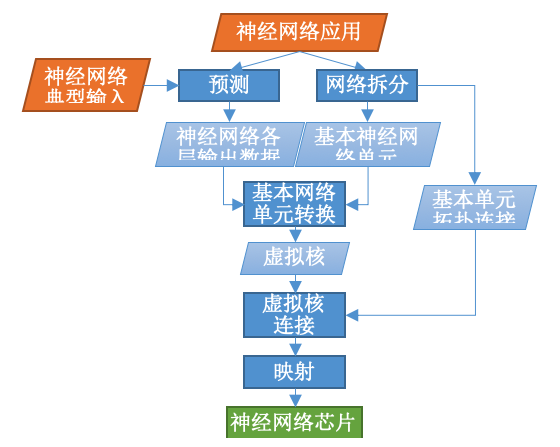
\includegraphics[width=0.60\textwidth]{Img/Chap_Application/Zhang/Systemflow.png}
    \bicaption{系统流程图}{系统流程图}\label{fig:Systemflow}
\end{figure}


\begin{itemize}
    \item 基本神经网络单元\\
    如图\ref{fig:NNUint},基本的神经网络单元为输入为n个神经元,输出为m个神经元,输入神经元与输出神经元之间全相联,若不是全相连,可以以将未相连的边看作连接权重是0的边。通过将复杂神经网络拆成基本神经网络单元,再通过对基本神经网络基本单元的转换,完成对整个神经网络的转换。
    \item 基本神经网络单元的转\\
    神经网络芯片的处理核的功能通常也是处理类似图\ref{fig:NNUint}的结构,但通常输入和输出的数量是固定的,例如IBM的TrueNorth芯片,其神经突触核支持的输入和输出数量均为256。但应用层的基本神经网络单元输入输出节点数量通常远大于硬件所支持的输入输出数量。此外,硬件的权重位宽和输入输出数据通常较低,且常常用整数或定点数来表示。此外,硬件所支持的激活函数或神经元模型通常非常简单,且是固定的。因此基本神经网络单元的转换主要需要解决如下3个硬件带来的约束:连接度约束,即输入输出的数量;精度约束,包括权重以及其他参数的精度和输入输出数据的精度;激活函数或神经元模型的约束。
    
    \begin{figure}[!htbp]
    \centering
    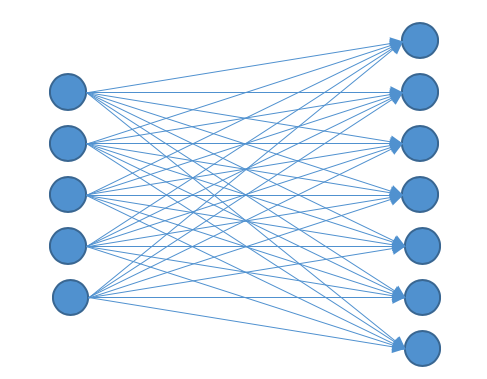
\includegraphics[width=0.60\textwidth]{Img/Chap_Application/Zhang/NNUint.png}
    \bicaption{神经网络基本单元}{神经网络基本单元}\label{fig:NNUint}
    \end{figure}
    
    分别通过权重矩阵稀疏化、低精度训练和插入隐藏层来解决上述三种约束。对基本神经网络单元的训练流程如图\ref{fig:NNUintExchange}所示。

    \begin{figure}[!htbp]
    \centering
    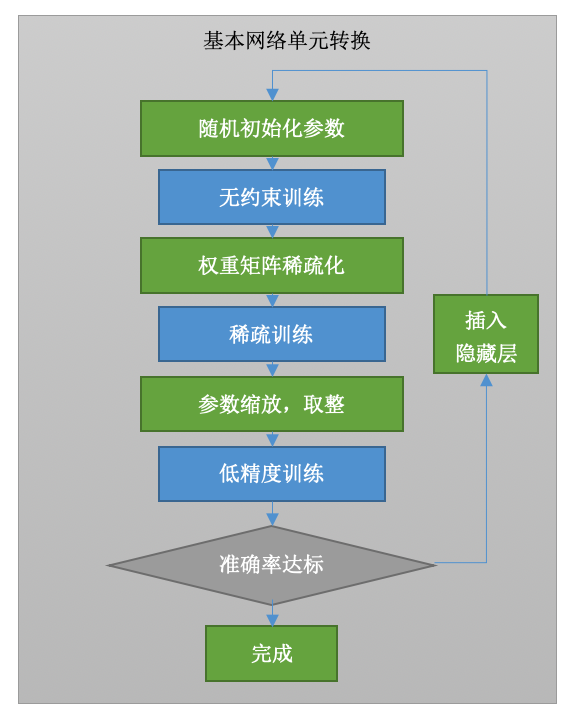
\includegraphics[width=0.60\textwidth]{Img/Chap_Application/Zhang/NNUintExchange.png}
    \bicaption{神经网络基本单元转换流程}{神经网络基本单元转换流程}\label{fig:NNUintExchange}
    \end{figure}

    对于n个输入,m个输出的基本神经网络单元,构建一个输入层为n个,输出层为m个,输入输出之间全相联的神经网络,神经元模型或激活函数使用神经网络硬件所支持的。用基本神经网络单元的典型输入输出数据来训练构建的神经网络。
    
    首先随机初始化参数,不加任何约束地训练这个网络,若硬件所支持的是ANN,则使用经典的随机梯度下降来训练,如果硬件所支持的是SNN,则使用其spike发放频率作为输入输出数据,同样适用随机梯度下降来训练,训练之后使得网络对输入的预测结果与对于的输出尽可能接近。
    
    若n超过了硬件所允许的最大输入k或者m超过了硬件所允许的最大输出l,则进行权重矩阵稀疏化。如图\ref{fig:matrix}所示,在权重矩阵的对焦线上选择一系列子矩阵,使得每个子矩阵的大小均满足硬件的输入输出限制。通过不断交换矩阵的行或列,或者将其中某一行或某一列从一个子矩阵移到另一个子矩阵,使得所有子矩阵中的权重的绝对值总和最大。
    
    \begin{figure}[!htbp]
    \centering
    \includegraphics[width=0.65\textwidth]{Img/Chap_Application/Zhang/matrix.png}
    \bicaption{权重矩阵稀疏化}{权重矩阵稀疏化}\label{fig:matrix}
    \end{figure}
    
    经过稀疏化之后,所有子矩阵之外的权重均强制设置为0,并以此为约束重新训练。训练完之后,根据神经元模型,在不影响结果的情况下,将所有的参数线性缩放,使得所有的参数刚好落在神经网络硬件的精度范围内,并四舍五入到硬件的精度。重新训练网络,所有参数在训练时保存为浮点数,在训练前馈过程中,首先将所有参数四舍五入到硬件的精度,在反馈和更新的过程中,使用仍然采用浮点数。
    
    若低精度训练之后,网络的准确率不能达到预期的要求,则在输入层和输出层之间增加隐藏层,重复上述步骤,直到网络的准确率能达到预期的要求为止。
    
    此时得到的网络已经满足硬件的所有约束条件,权重矩阵稀疏化过程中的每个子矩阵看作一个虚拟核,与神经网络芯片中的一个核相对应。
    
    \item 复杂网络拆分和逐层转换
    
    这儿将介绍对于任意的复杂网络,如何拆分成基本神经网络单元。 
    
    \begin{figure}[!htbp]
    \centering
    \includegraphics[width=0.60\textwidth]{Img/Chap_Application/Zhang/MNsplit.png}
    \bicaption{复杂网络的拆分}{复杂网络的拆分}\label{fig:MNsplit}
    \end{figure}
    
    复杂神经网络以层为基本单元,每层神经元包含若干神经元,层与层之间相互连接,形成一个有向图,如图\ref{fig:MNsplit}(A)所示。

    对于有向图中任意节点$P_a$,若$P_a$有n个后向节点,则引加入一个多播层$P_na$,该多播层由n个$P_a$拼接而成,如图\ref{fig:MNsplit}(B)所示,$P_a$与$P_na$之间的连接为基本神经网络单元,$P_na$中的每一份$P_a$分别与一个后向节点相连。
    
    对于有向图中任意节点$P_a$,若$P_a$有n个前向节点(已增加完多播层),如图\ref{fig:MNsplit}(C)所示,将Pa的所有前向节点拼接在一起当作一层$P_pre$,此时$P_a$与$P_pre$之间的连接为基本神经网络单元。
    
    经过了上述步骤,可以将复杂神经网络拆分成基本神经网络单元,进而利用前面所述的转换方法拆分成若干虚拟核。例如图\ref{fig:MNsplit}(A)中所示的神经网络被拆分成了图\ref{fig:MNsplit}(D)中所示结构,其中图\ref{fig:MNsplit}(D)种每个箭头表示一个基本神经网络单元。
    
    神经网络的典型输入从输入层输入,在原神经网络的每一层产生相应的输出,为基本神经网络单元的转换提供训练数据。
    
    由于基本神经网络单元的转换会有误差,为了避免误差的逐层积累。对于有向无环图,对图进行拓扑排序,按照拓扑排序的顺序逐层进行转换,每个基本神经网络单元转换完在之后,利用其输入和训练出的权重等参数生成其输出,并以该输出作为后续基本神经网络单元训练时的输入数据。对于有环图,切断其中若干条边使得图中所有的环消失,然后对其进行拓扑排序,并按照该顺序进行基本神经网络单元的转换,若基本神经网络单元的部分输入来自切断的边,则利用原神经网络每一层产生的输出作为这部分输入的数据。
    
    \item 虚拟核的连接和映射
    
    经过上述步骤,复杂神经网络被拆分为基本神经网络单元,并按照拓扑排序的顺序进行逐层转换,最终得到了若干虚拟核,根据拆分和权重矩阵稀疏化步骤的连接信息,将这些虚拟核连接起来,得到虚拟核的连接图,利用经典的片上网络的映射算法(例如KL算法)将虚拟核与芯片上的物理核一一对应,将各个虚拟核的参数配置到对应的物理核上,完成神经网络的转换。
    
    \item 神经网络编译精度\\
    (补充数据)

\end{itemize}

(2)支持基本神经网络单元的可重构神经网络加速器设计

(1)中引入了神经网络和芯片之间的数据流图形式的中间层,中间层的计算单元是基本神经网络单元,该单元的计算主题是向量矩阵乘,因此证明这一软硬件去耦合设计思路优越性的关键是能否设计支持这类基本神经网络单元的高效加速器结构,尤其是考虑到(1)中的神经网络编译会增大神经网络的规模,这就使得支持基本神经网络单元的高效硬件设计尤为重要。

本节基于具有高密度、高能效向量矩阵乘计算能力的ReRAM交叉开关结构,同时针对神经网络内部的数据通信特性提出采用可重构片上互连机制,并引入可重构逻辑实现数据流计算图的片上控制功能,从而提出可重构神经网络加速器设计,称为FPSA(Field Programmable Synapse Array)。

仿真测试表明,该设计的网络推断性能较同样基于ReRAM交叉开关结构的PRIME加速器结构提升1000倍。

\begin{itemize}
    \item ReRAM与基本神经网络单元
    ReRAM(resistive random-access memory,非易失性阻变存储器)是新一代的多级(Multi-level)存储器件,理论上可以将ReRAM的电导值设为其取值范围中的任意值。我们可以将ReRAM在Crossba交叉点的阻值设置为神经网络权重矩阵的对应值,这样就可以用一个ReRAM Crossbar来表示一个神经网络的权重矩阵,并且根据其物理特性就地(in-situ)完成矩阵向量乘操作。对于理想的Crossbar器件,将输入电压$V_i$加到每一行(字线,word-line),电压与每一交叉点的电导值$G_ij$ 相乘,根据基尔霍夫定律$I=GV$,每一列的输出电流$I$ 可累加得到,该计算过程能达到很高的并行度和速度。本设计中就是以高密度、高能效的ReRAM交叉开关结构作为基本神经网络单元的基础实现。(附图)
    
    \includegraphics[scale=0.6]{Img/Chap_Application/Zhang/ReRAM.png}
    
    \item 可重构神经网络加速器结构设计\\
    
    With the hierarchical software system, we propose the compact and efficient FPSA architecture. FPSA is a reconfigurable architecture composed of three kinds of functional blocks: ReRAM-based PE, Spiking Memory Block (SMB), and Configurable Logic Block (CLB). ReRAM-based Processing Element (PE). Due to the transformation of neural synthesizer, the PE only needs to support the HEM IR with ReRAM-crossbar. To further reduce the overhead of ADC/DAC, we employ spiking schema, which uses the spike count of 1-bit spikes to represent input/output data. And the corresponding ReLU function can be implemented with a simplified Integrate-and-Fire (IF) neuron model. We propose a compact circuit design to enable core-op computation with the spiking schema.
    
    Spiking Memory Block (SMB). Since PEs communicate with 1-bit spikes, we propose SMB to buffer the information. It integrates the spike counter and generator together with the memory array to enable efficient load and store of spike counts. Configurable Logic Block (CLB). As mentioned above, to enable flexible and temporal scheduling of the spatial-to-temporal mapper, we introduce CLB widely used in FPGA to implement control logic. Till now, FPSA provides massive functional blocks for the software system. Further, to match the high throughput of PE, we use a reconfigurable routing architecture composed of plenty of wiring resources and configurable switches to connect these functional blocks together.

    Accordingly, neural synthesizer, one tool of the proposed software system, can convert an NN in the SPM form into an equivalent CG of core-ops. Thus, we can support NN frameworks flexibly and the hardware only needs to support core-op, which greatly simplifies the circuit design of FPSA. Further, we integrate reconfigurable buffer resources and control logic in hardware and introduce a spatial-to-temporal mapper in software. The latter schedules the execution of HEM and turns it into a netlist composed of the PEs, the buffers and control logic. Finally, to match the high throughput of the ReRAM-based PEs, we propose a reconfigurable routing architecture as the interconnection subsystem to supply extremely high bandwidth and low latency. At the same time, a placement \& routing tool is leveraged to place the netlist onto hardware and generate the routing configuration.

    Compared to one state-of-the-art ReRAM-based NN accelerator, PRIME [9], our approach improves the performance by up to 1000× for representative NN models and the accuracy loss is negligible. 
\end{itemize}

(参考文献:Bridging the Gap Between Neural Networks and Neuromorphic Hardware with A Neural Network Compiler,ASPLOS 2018论文;

FPSA: A Full System Stack Solution for Reconfigurable ReRAM-based NN Accelerator Architecture,ASPLOS 2019论文)

\subsection{相关工作}
(根据上述具体工作再做相关展开)


\section{数据流模型在大数据分析中的应用(郑龙)}
\subsection{引言}
\subsection{……}
\subsection{……}
\subsection{相关工作}
\section{总结与评述}
\section{文献索引和笔记}


\end{flushleft}
 %%第五章
\chapter{相关工作}\label{chap:related}

<作者:G.R. Gao and ...>
%%\section{研究背景}

%%XXX
 %%第六章
\chapter{总结与未来方向}\label{chap:summary}

<作者:G.R. Gao and J.B. Dennis>
%%\section{研究背景}

%%XXX
 %%第七章

%---------------------------------------------------------------------------%
% main content

%-
%-> Appendix
%-
\cleardoublepage%
%%\appendix% initialize the environment
%%\chapter{中国科学院大学学位论文撰写要求}

学位论文是研究生科研工作成果的集中体现,是评判学位申请者学术水平、授予其学位的主要依据,是科研领域重要的文献资料。根据《科学技术报告、学位论文和学术论文的编写格式》(GB/T 7713-1987)、《学位论文编写规则》(GB/T 7713.1-2006)和《文后参考文献著录规则》(GB7714—87)等国家有关标准,结合中国科学院大学(以下简称“国科大”)的实际情况,特制订本规定。

\section{论文无附录者无需附录部分}

\section{测试公式编号 \texorpdfstring{$\Lambda,\lambda,\theta,\bar{\Lambda},\sqrt{S_{NN}}$}{$\textLambda,\textlambda,\texttheta,\bar{\textLambda},\sqrt{S_{NN}}$}} \label{sec:testmath}

\begin{equation} \label{eq:appedns}
    \adddotsbeforeeqnnum%
    \begin{cases}
        \frac{\partial \rho}{\partial t} + \nabla\cdot(\rho\Vector{V}) = 0\\
        \frac{\partial (\rho\Vector{V})}{\partial t} + \nabla\cdot(\rho\Vector{V}\Vector{V}) = \nabla\cdot\Tensor{\sigma}\\
        \frac{\partial (\rho E)}{\partial t} + \nabla\cdot(\rho E\Vector{V}) = \nabla\cdot(k\nabla T) + \nabla\cdot(\Tensor{\sigma}\cdot\Vector{V})
    \end{cases}
\end{equation}
\begin{equation}
    \adddotsbeforeeqnnum%
    \frac{\partial }{\partial t}\int\limits_{\Omega} u \, \mathrm{d}\Omega + \int\limits_{S} \unitVector{n}\cdot(u\Vector{V}) \, \mathrm{d}S = \dot{\phi}
\end{equation}
\[
    \begin{split}
        \mathcal{L} \{f\}(s) &= \int _{0^{-}}^{\infty} f(t) e^{-st} \, \mathrm{d}t, \ 
        \mathscr{L} \{f\}(s) = \int _{0^{-}}^{\infty} f(t) e^{-st} \, \mathrm{d}t\\
        \mathcal{F} {\bigl (} f(x+x_{0}) {\bigr )} &= \mathcal{F} {\bigl (} f(x) {\bigr )} e^{2\pi i\xi x_{0}}, \ 
        \mathscr{F} {\bigl (} f(x+x_{0}) {\bigr )} = \mathscr{F} {\bigl (} f(x) {\bigr )} e^{2\pi i\xi x_{0}}
    \end{split}
\]

mathtext: $A,F,L,2,3,5,\sigma$, mathnormal: $A,F,L,2,3,5,\sigma$, mathrm: $\mathrm{A,F,L,2,3,5,\sigma}$.

mathbf: $\mathbf{A,F,L,2,3,5,\sigma}$, mathit: $\mathit{A,F,L,2,3,5,\sigma}$, mathsf: $\mathsf{A,F,L,2,3,5,\sigma}$.

mathtt: $\mathtt{A,F,L,2,3,5,\sigma}$, mathfrak: $\mathfrak{A,F,L,2,3,5,\sigma}$, mathbb: $\mathbb{A,F,L,2,3,5,\sigma}$.

mathcal: $\mathcal{A,F,L,2,3,5,\sigma}$, mathscr: $\mathscr{A,F,L,2,3,5,\sigma}$, boldsymbol: $\boldsymbol{A,F,L,2,3,5,\sigma}$.

vector: $\Vector{\sigma, T, a, F, n}$, unitvector: $\unitVector{\sigma, T, a, F, n}$

matrix: $\Matrix{\sigma, T, a, F, n}$, unitmatrix: $\unitMatrix{\sigma, T, a, F, n}$

tensor: $\Tensor{\sigma, T, a, F, n}$, unittensor: $\unitTensor{\sigma, T, a, F, n}$ 

\section{测试生僻字}

霜蟾盥薇曜灵霜颸妙鬘虚霩淩澌菀枯菡萏泬寥窅冥毰毸濩落霅霅便嬛岧峣瀺灂姽婳愔嫕飒纚棽俪緸冤莩甲摛藻卮言倥侗椒觞期颐夜阑彬蔚倥偬澄廓簪缨陟遐迤逦缥缃鹣鲽憯懔闺闼璀错媕婀噌吰澒洞阛闠覼缕玓瓑逡巡諓諓琭琭瀌瀌踽踽叆叇氤氲瓠犀流眄蹀躞赟嬛茕頔璎珞螓首蘅皋惏悷缱绻昶皴皱颟顸愀然菡萏卑陬纯懿犇麤掱暒 墌墍墎墏墐墒墒墓墔墕墖墘墖墚墛坠墝增墠墡墢墣墤墥墦墧墨墩墪樽墬墭堕墯墰墱墲坟墴墵垯墷墸墹墺墙墼墽垦墿壀壁壂壃壄壅壆坛壈壉壊垱壌壍埙壏壐壑壒压壔壕壖壗垒圹垆壛壜壝垄壠壡坜壣壤壥壦壧壨坝塆圭嫶嫷嫸嫹嫺娴嫼嫽嫾婳妫嬁嬂嬃嬄嬅嬆嬇娆嬉嬊娇嬍嬎嬏嬐嬑嬒嬓嬔嬕嬖嬗嬘嫱嬚嬛嬜嬞嬟嬠嫒嬢嬣嬥嬦嬧嬨嬩嫔嬫嬬奶嬬嬮嬯婴嬱嬲嬳嬴嬵嬶嬷婶嬹嬺嬻嬼嬽嬾嬿孀孁孂娘孄孅孆孇孆孈孉孊娈孋孊孍孎孏嫫婿媚嵭嵮嵯嵰嵱嵲嵳嵴嵵嵶嵷嵸嵹嵺嵻嵼嵽嵾嵿嶀嵝嶂嶃崭嶅嶆岖嶈嶉嶊嶋嶌嶍嶎嶏嶐嶑嶒嶓嵚嶕嶖嶘嶙嶚嶛嶜嶝嶞嶟峤嶡峣嶣嶤嶥嶦峄峃嶩嶪嶫嶬嶭崄嶯嶰嶱嶲嶳岙嶵嶶嶷嵘嶹岭嶻屿岳帋巀巁巂巃巄巅巆巇巈巉巊岿巌巍巎巏巐巑峦巓巅巕岩巗巘巙巚帠帡帢帣帤帨帩帪帬帯帰帱帲帴帵帷帹帺帻帼帽帾帿幁幂帏幄幅幆幇幈幉幊幋幌幍幎幏幐幑幒幓幖幙幚幛幜幝幞帜幠幡幢幤幥幦幧幨幩幪幭幮幯幰幱庍庎庑庖庘庛庝庠庡庢庣庤庥庨庩庪庬庮庯庰庱庲庳庴庵庹庺庻庼庽庿廀厕廃厩廅廆廇廋廌廍庼廏廐廑廒廔廕廖廗廘廙廛廜廞庑廤廥廦廧廨廭廮廯廰痈廲廵廸廹廻廼廽廿弁弅弆弇弉弖弙弚弜弝弞弡弢弣弤弨弩弪弫弬弭弮弰弲弪弴弶弸弻弼弽弿彖彗彘彚彛彜彝彞彟彴彵彶彷彸役彺彻彽彾佛徂徃徆徇徉后徍徎徏径徒従徔徕徖徙徚徛徜徝从徟徕御徢徣徤徥徦徧徨复循徫旁徭微徯徰徱徲徳徴徵徶德徸彻徺忁忂惔愔忇忈忉忔忕忖忚忛応忝忞忟忪挣挦挧挨挩挪挫挬挭挮挰掇授掉掊掋掍掎掐掑排掓掔掕挜掚挂掜掝掞掟掠采探掣掤掦措掫掬掭掮掯掰掱掲掳掴掵掶掸掹掺掻掼掽掾掿拣揁揂揃揅揄揆揇揈揉揊揋揌揍揎揑揓揔揕揖揗揘揙揤揥揦揧揨揫捂揰揱揲揳援揵揶揷揸揻揼揾揿搀搁搂搃搄搅搇搈搉搊搋搌搎搏搐搑搒摓摔摕摖摗摙摚摛掼摝摞摠摡斫斩斮斱斲斳斴斵斶斸旪旫旮旯晒晓晔晕晖晗晘晙晛晜晞晟晠晡晰晣晤晥晦晧晪晫晬晭晰晱晲晳晴晵晷晸晹晻晼晽晾晿暀暁暂暃暄暅暆暇晕晖暊暋暌暍暎暏暐暑暒暓暔暕暖暗旸暙暚暛暜暝暞暟暠暡暣暤暥暦暧暨暩暪暬暭暮暯暰昵暲暳暴暵暶暷暸暹暺暻暼暽暾暿曀曁曂曃晔曅曈曊曋曌曍曎曏曐曑曒曓曔曕曗曘曙曚曛曜曝曞曟旷曡曢曣曤曥曦曧昽曩曪曫晒曭曮曯椗椘椙椚椛検椝椞椟椠椡椢椣椤椥椦椧椨椩椪椫椬椭椮。
% appendix content

%-
%-> Backmatter: bibliography, glossary, index
%-
%%\backmatter% initialize the environment
%%\intotoc*{\cleardoublepage}{\bibname}% add link to toc
%%\bibliography{Biblio/ref}% bibliography
%%%---------------------------------------------------------------------------%
%->> Backmatter
%---------------------------------------------------------------------------%
\chapter{作者简历及攻读学位期间发表的学术论文与研究成果}

\textbf{本科生无需此部分}。

\section*{作者简历}

\subsection*{casthesis作者}

吴凌云,福建省屏南县人,中国科学院数学与系统科学研究院博士研究生。

\subsection*{ucasthesis作者}

莫晃锐,湖南省湘潭县人,中国科学院力学研究所硕士研究生。

\section*{已发表(或正式接受)的学术论文:}

[1] ucasthesis: A LaTeX Thesis Template for the University of Chinese Academy of Sciences, 2014.

\section*{申请或已获得的专利:}

(无专利时此项不必列出)

\section*{参加的研究项目及获奖情况:}

可以随意添加新的条目或是结构。

\chapter[致谢]{致\quad 谢}\chaptermark{致\quad 谢}% syntax: \chapter[目录]{标题}\chaptermark{页眉}
\thispagestyle{noheaderstyle}% 如果需要移除当前页的页眉
%\pagestyle{noheaderstyle}% 如果需要移除整章的页眉

感激casthesis作者吴凌云学长,gbt7714-bibtex-style
开发者zepinglee,和ctex众多开发者们。若没有他们的辛勤付出和非凡工作,\LaTeX{}菜鸟的我是无法完成此国科大学位论文\LaTeX{}模板ucasthesis的。在\LaTeX{}中的一点一滴的成长源于开源社区的众多优秀资料和教程,在此对所有\LaTeX{}社区的贡献者表示感谢!

ucasthesis国科大学位论文\LaTeX{}模板的最终成型离不开以霍明虹老师和丁云云老师为代表的国科大学位办公室老师们制定的官方指导文件和众多ucasthesis用户的热心测试和耐心反馈,在此对他们的认真付出表示感谢。特别对国科大的赵永明同学的众多有效反馈意见和建议表示感谢,对国科大本科部的陆晴老师和本科部学位办的丁云云老师的细致审核和建议表示感谢。谢谢大家的共同努力和支持,让ucasthesis为国科大学子使用\LaTeX{}撰写学位论文提供便利和高效这一目标成为可能。

\cleardoublepage[plain]% 让文档总是结束于偶数页,可根据需要设定页眉页脚样式,如 [noheaderstyle]
%---------------------------------------------------------------------------%
% other information
\end{document}
%---------------------------------------------------------------------------%

